\documentclass[letterpaper,12pt]{article}
\usepackage[utf8]{inputenc}
\usepackage[russian]{babel}
\usepackage[left=2cm,right=2cm,top=2cm,bottom=2cm,bindingoffset=0cm]{geometry}
\usepackage{graphicx}
\graphicspath{{images/}}
\usepackage{float}
\usepackage{wrapfig}

\begin{document}
\begin{center}
Построение <<нет-зоны>> отрезка
\end{center}
\par
Дан отрезок $p_1 p_2$, а также множество отрезков $S$.
Концы всех отрезков -- МТОП. Обозначим множество концов отрезков
из $S$ -- $P$.
\begin{figure}[H]
      \centering
      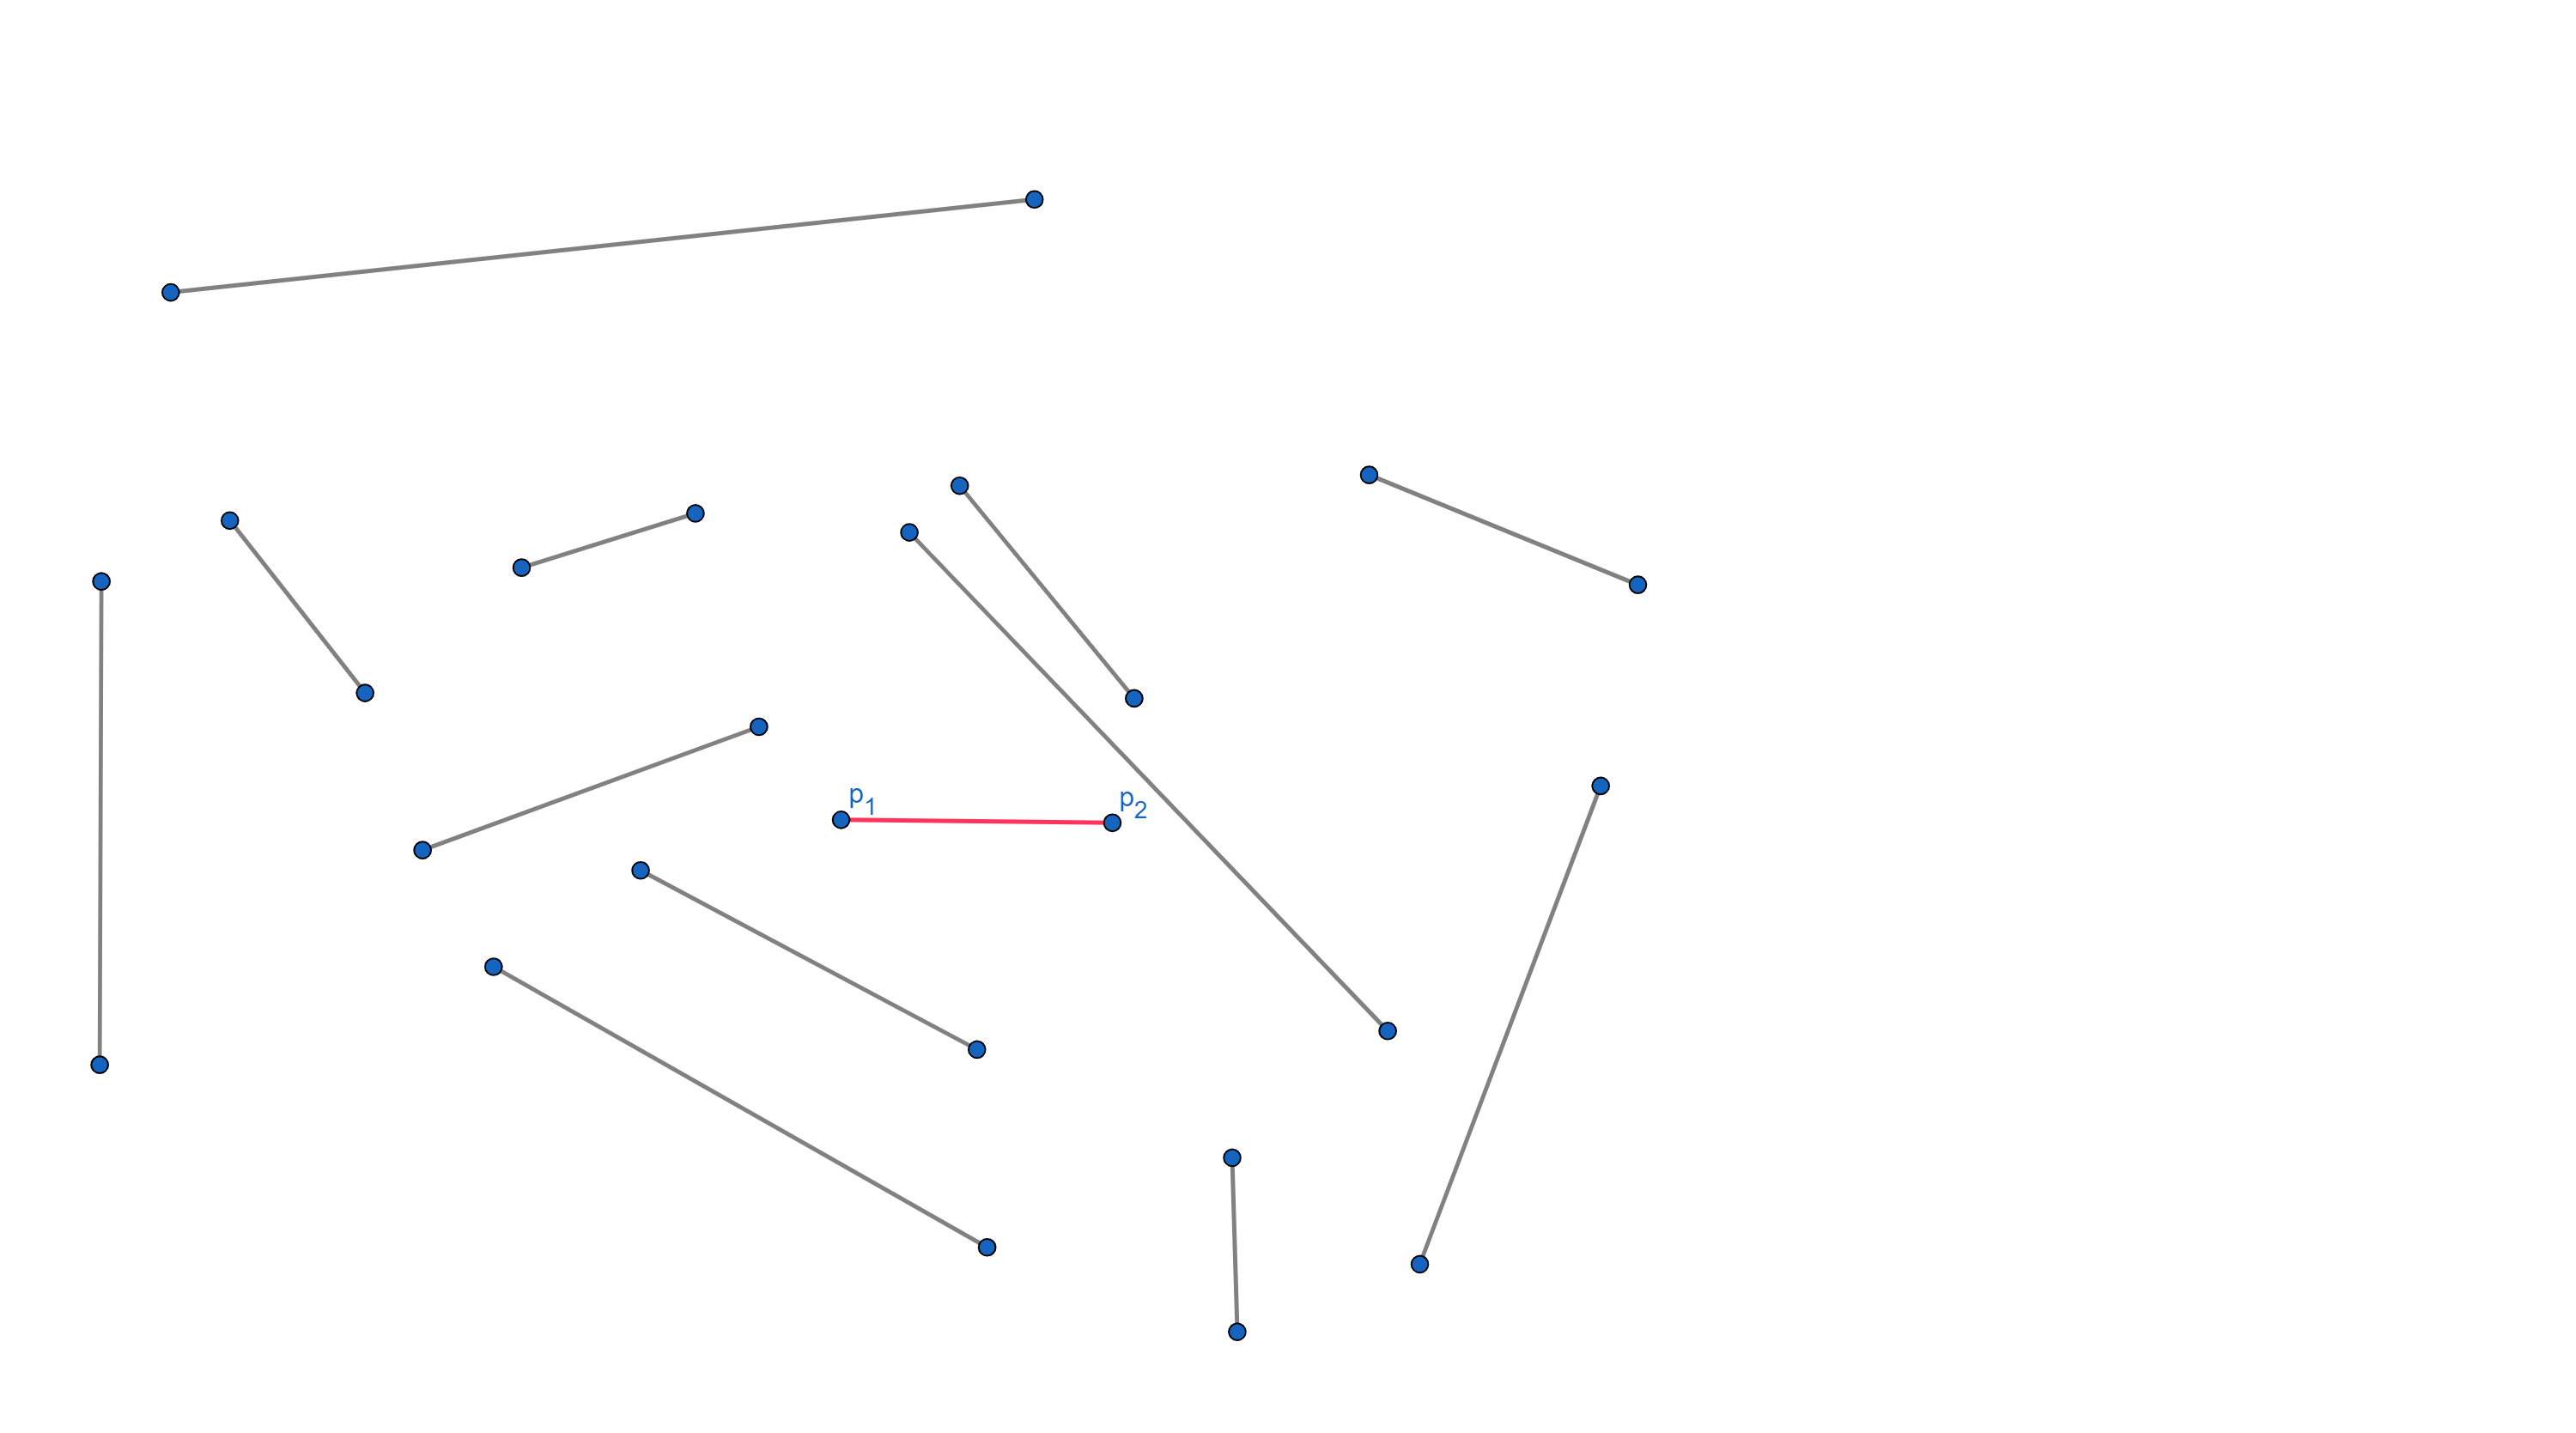
\includegraphics[width=0.5\linewidth]{segments_def.png}
\end{figure}
Все другие отрезки разобьем на 4 множества:
\begin{enumerate}
      \item Обе точки отрезка лежат слева от прямой, проведенной 
            через $p_1 p_2$. Обозначим $S_1$, концы -- $P_1$.
            \begin{figure}[H]
                  \centering
                  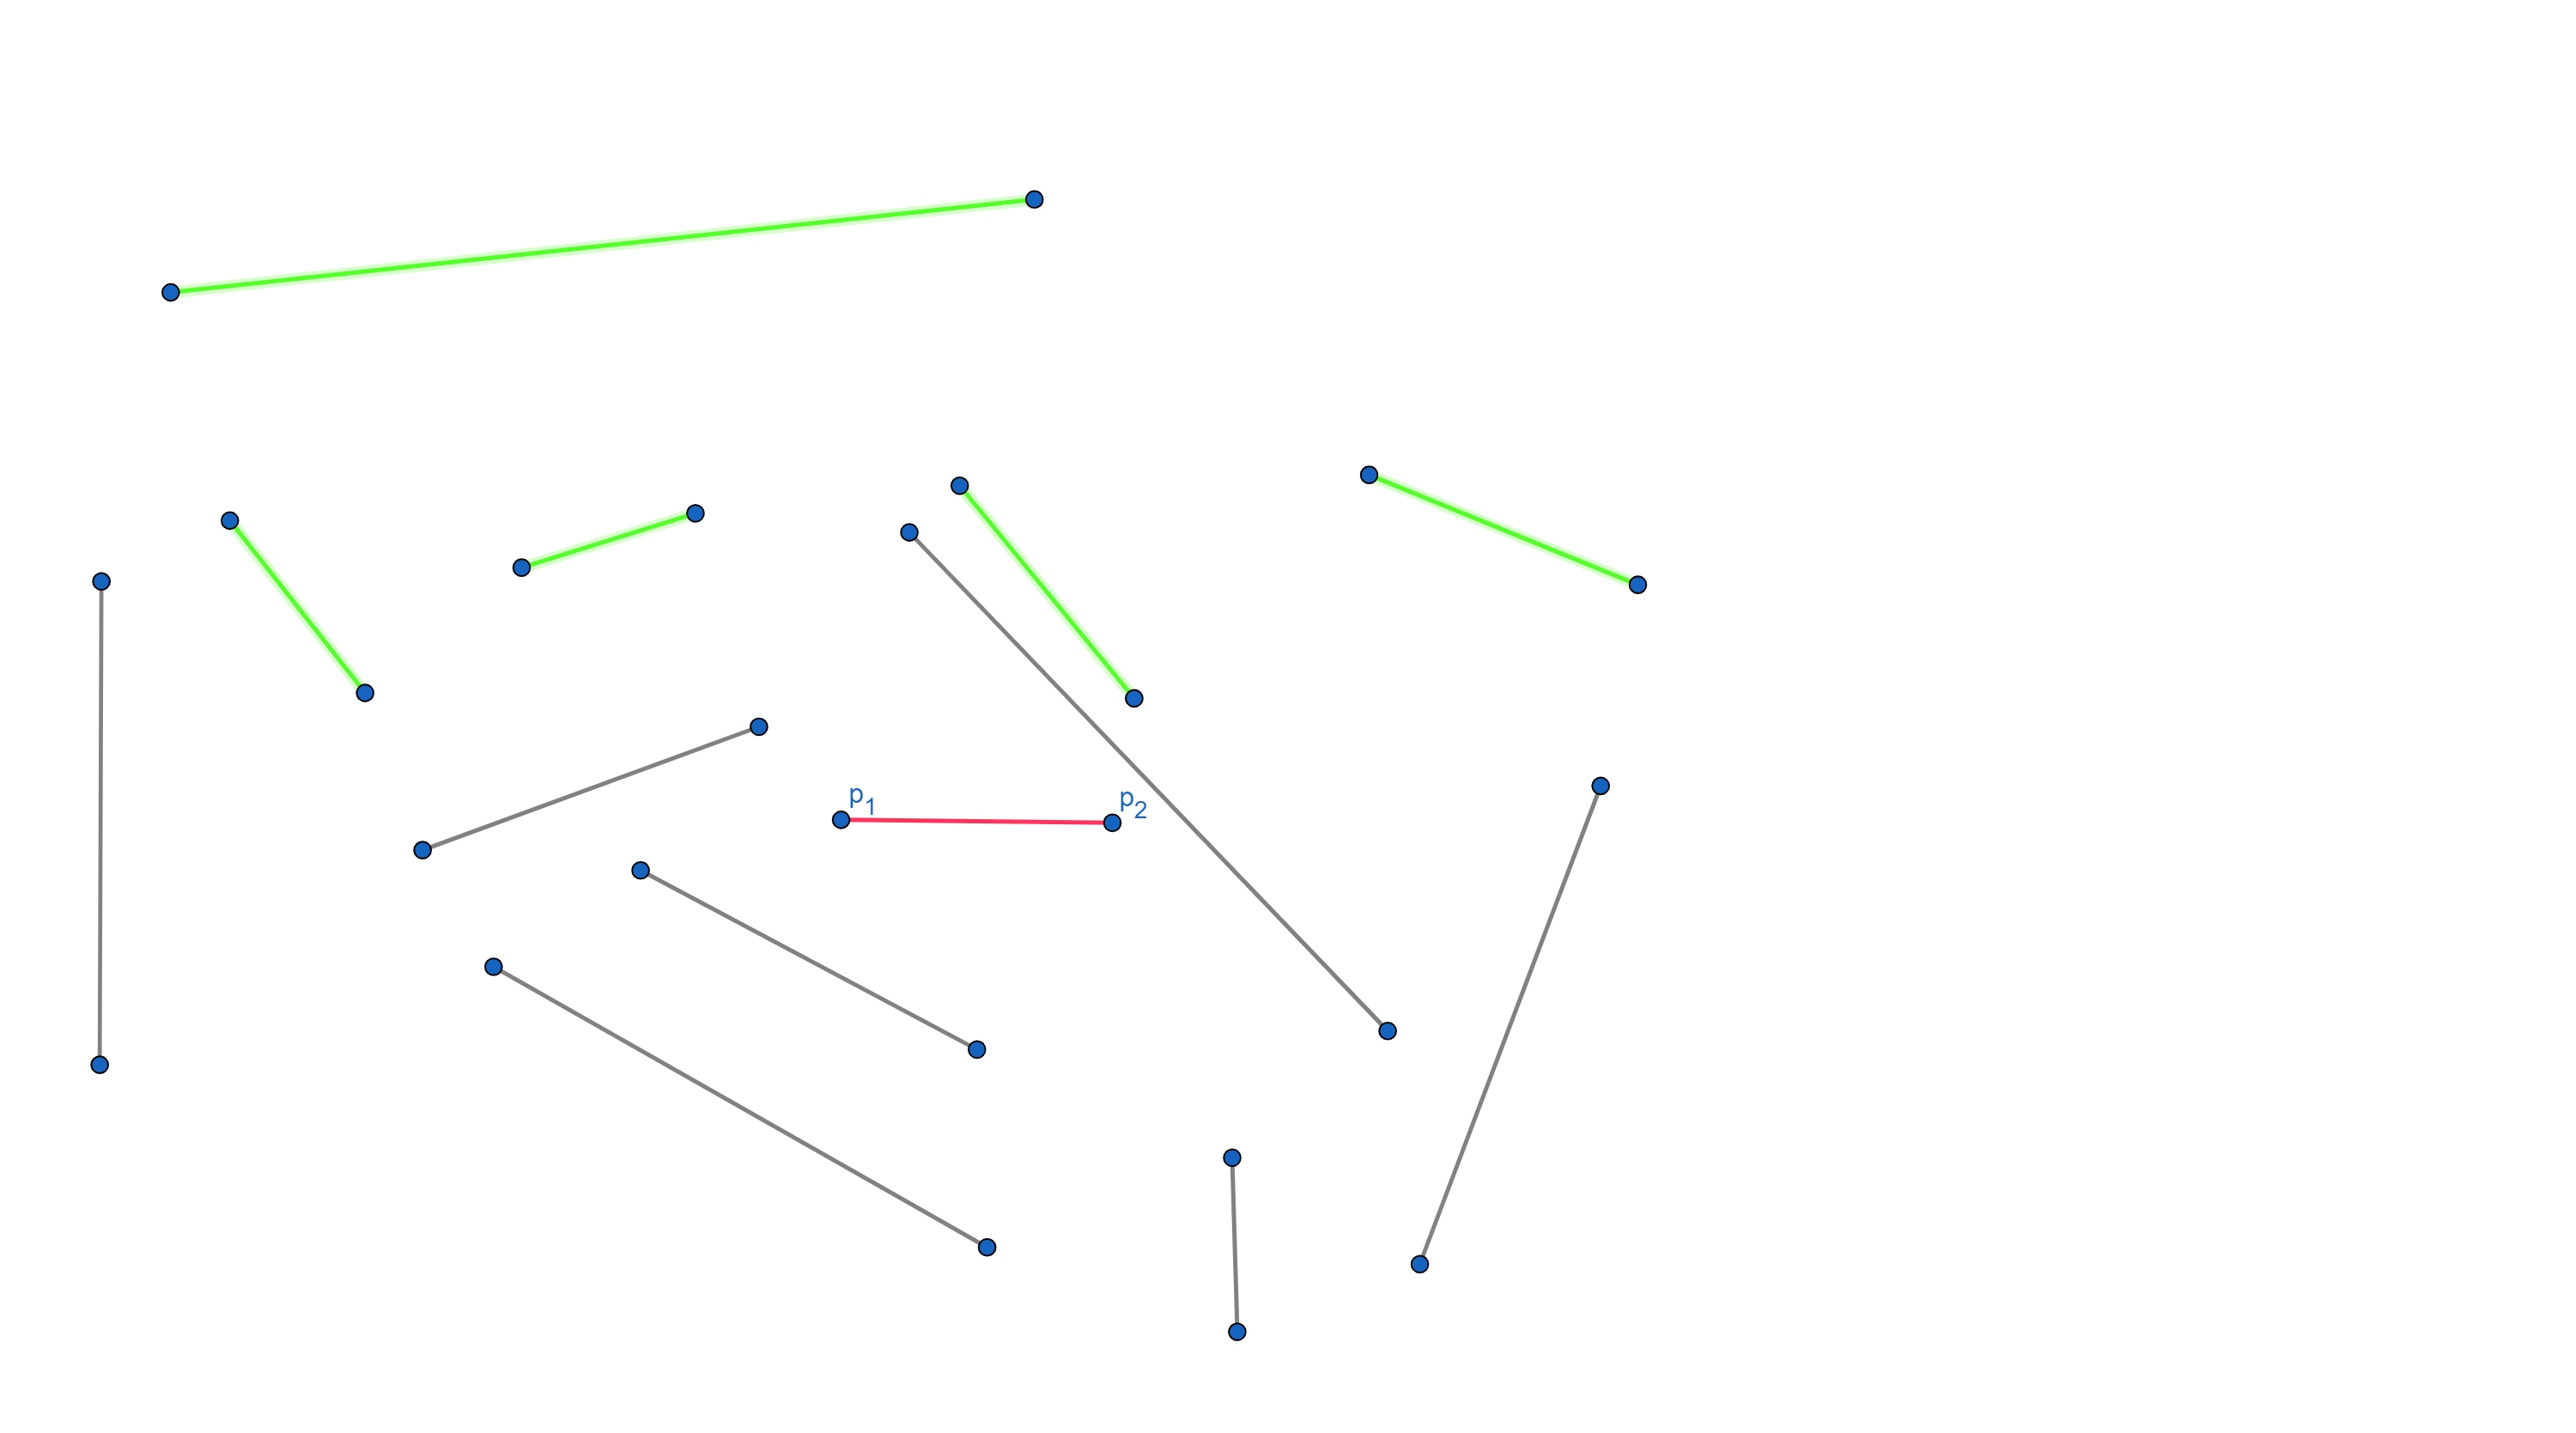
\includegraphics[width=0.5\linewidth]{segment_1.png}
            \end{figure}
      \item Обе точки отрезка лежат справа от прямой, проведенной 
            через $p_1 p_2$. Обозначим $S_2$, концы -- $P_2$.
            \begin{figure}[H]
                  \centering
                  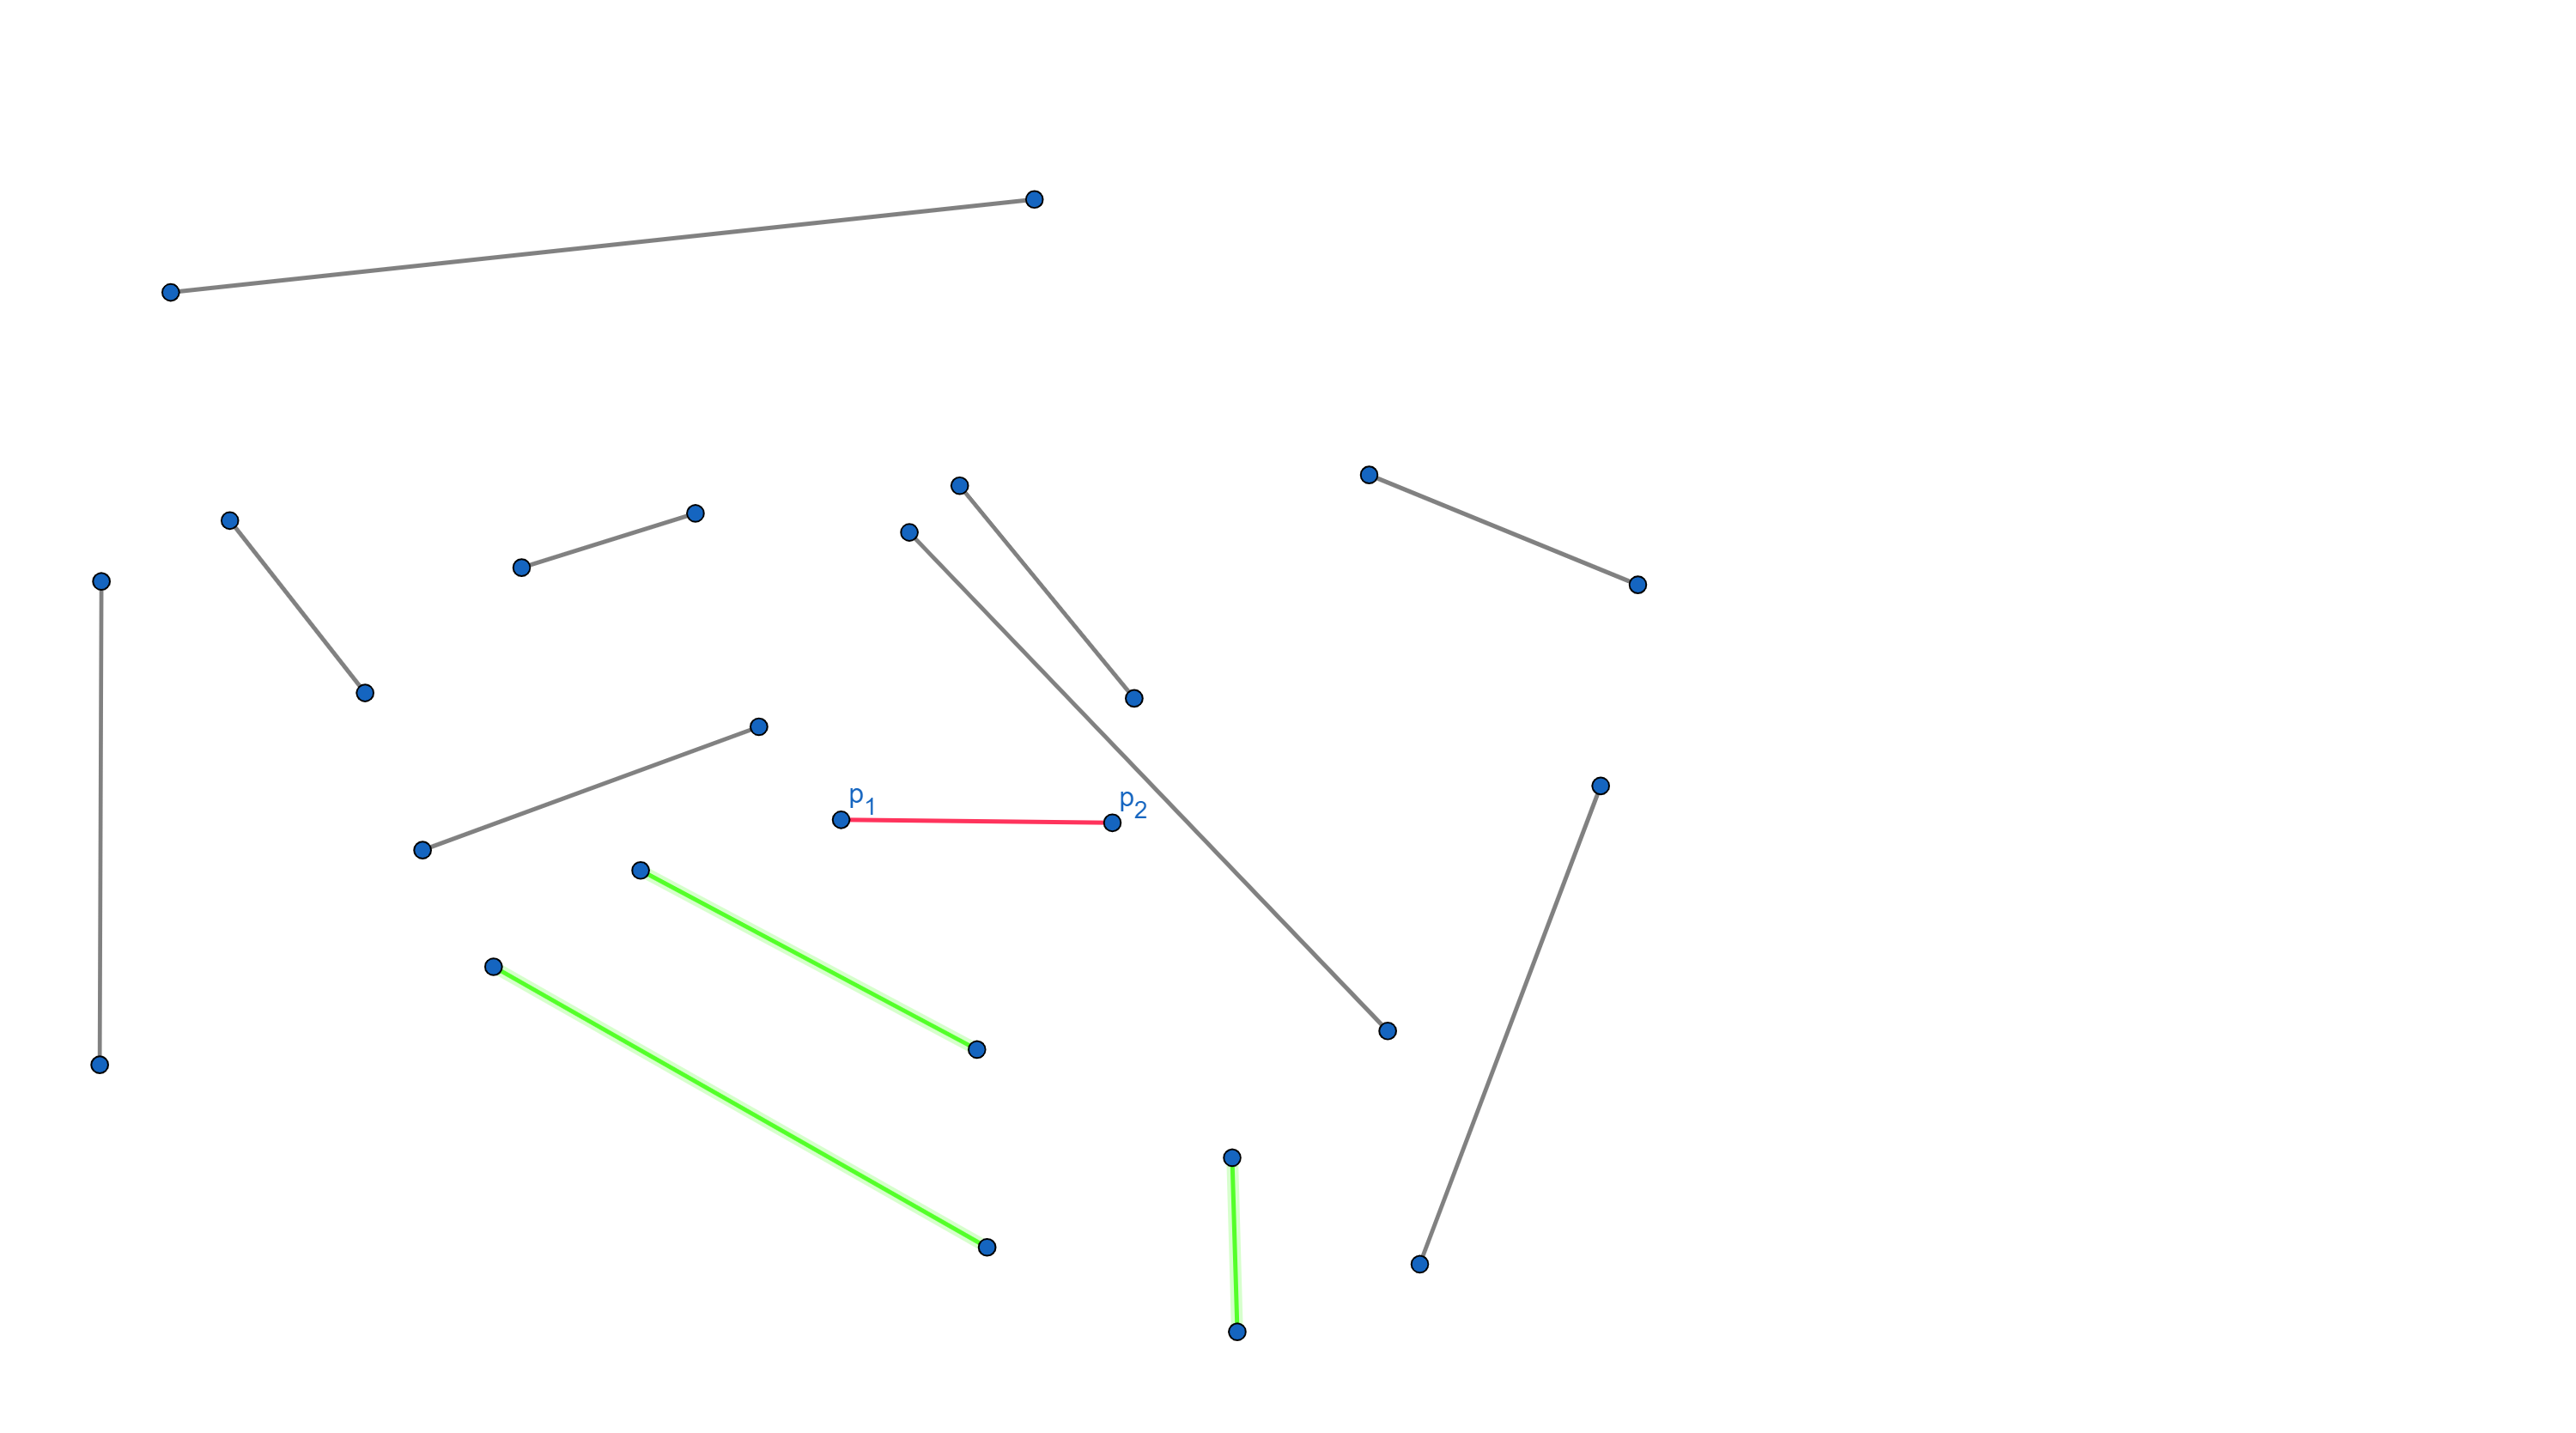
\includegraphics[width=0.5\linewidth]{segment_2.png}
            \end{figure}
            \pagebreak[3]
      \item Точки отрезка лежат по разные стороны от прямой, 
            проведенной через $p_1 p_2$. Отрезок пересекает
            данную прямую со стороны точки $p_1$. 
            Обозначим $S_3$, концы -- $P_3$.
            \begin{figure}[H]
                  \centering
                  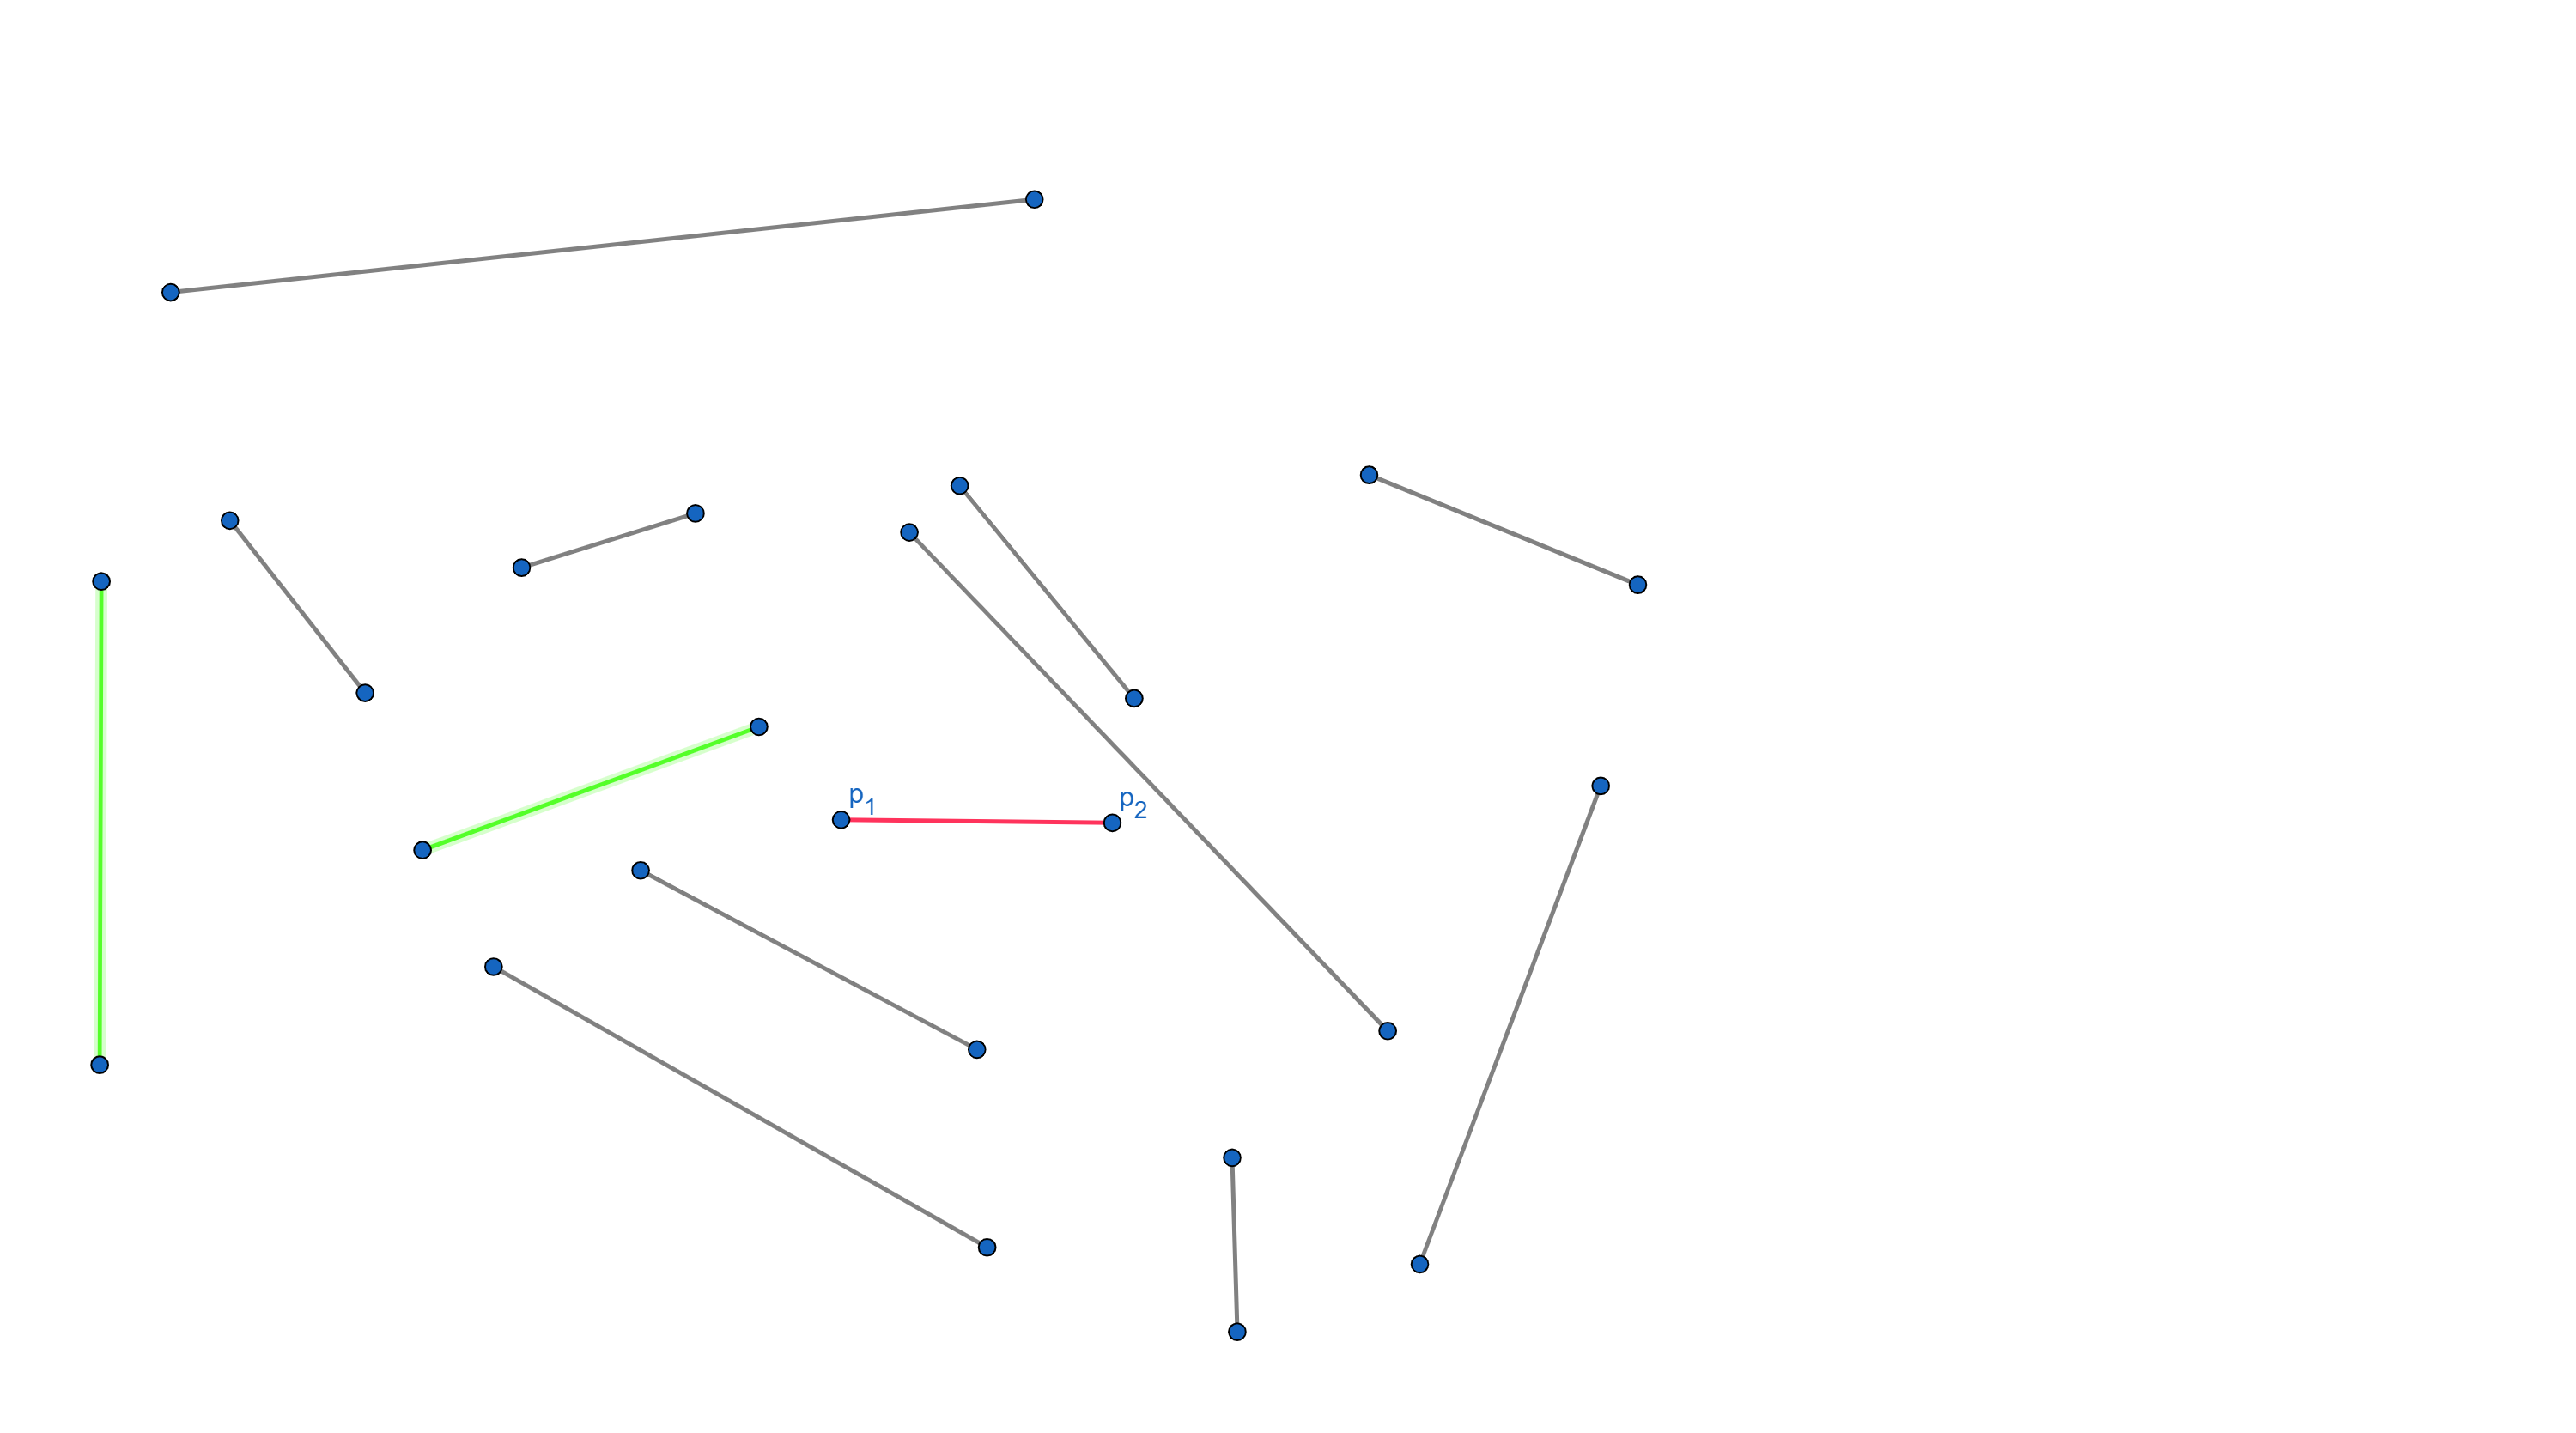
\includegraphics[width=0.5\linewidth]{segment_3.png}
            \end{figure}
      \item Точки отрезка лежат по разные стороны от прямой, 
            проведенной через $p_1 p_2$. Отрезок пересекает
            данную прямую со стороны точки $p_2$.
            Обозначим $S_4$, концы -- $P_4$.
            \begin{figure}[H]
                  \centering
                  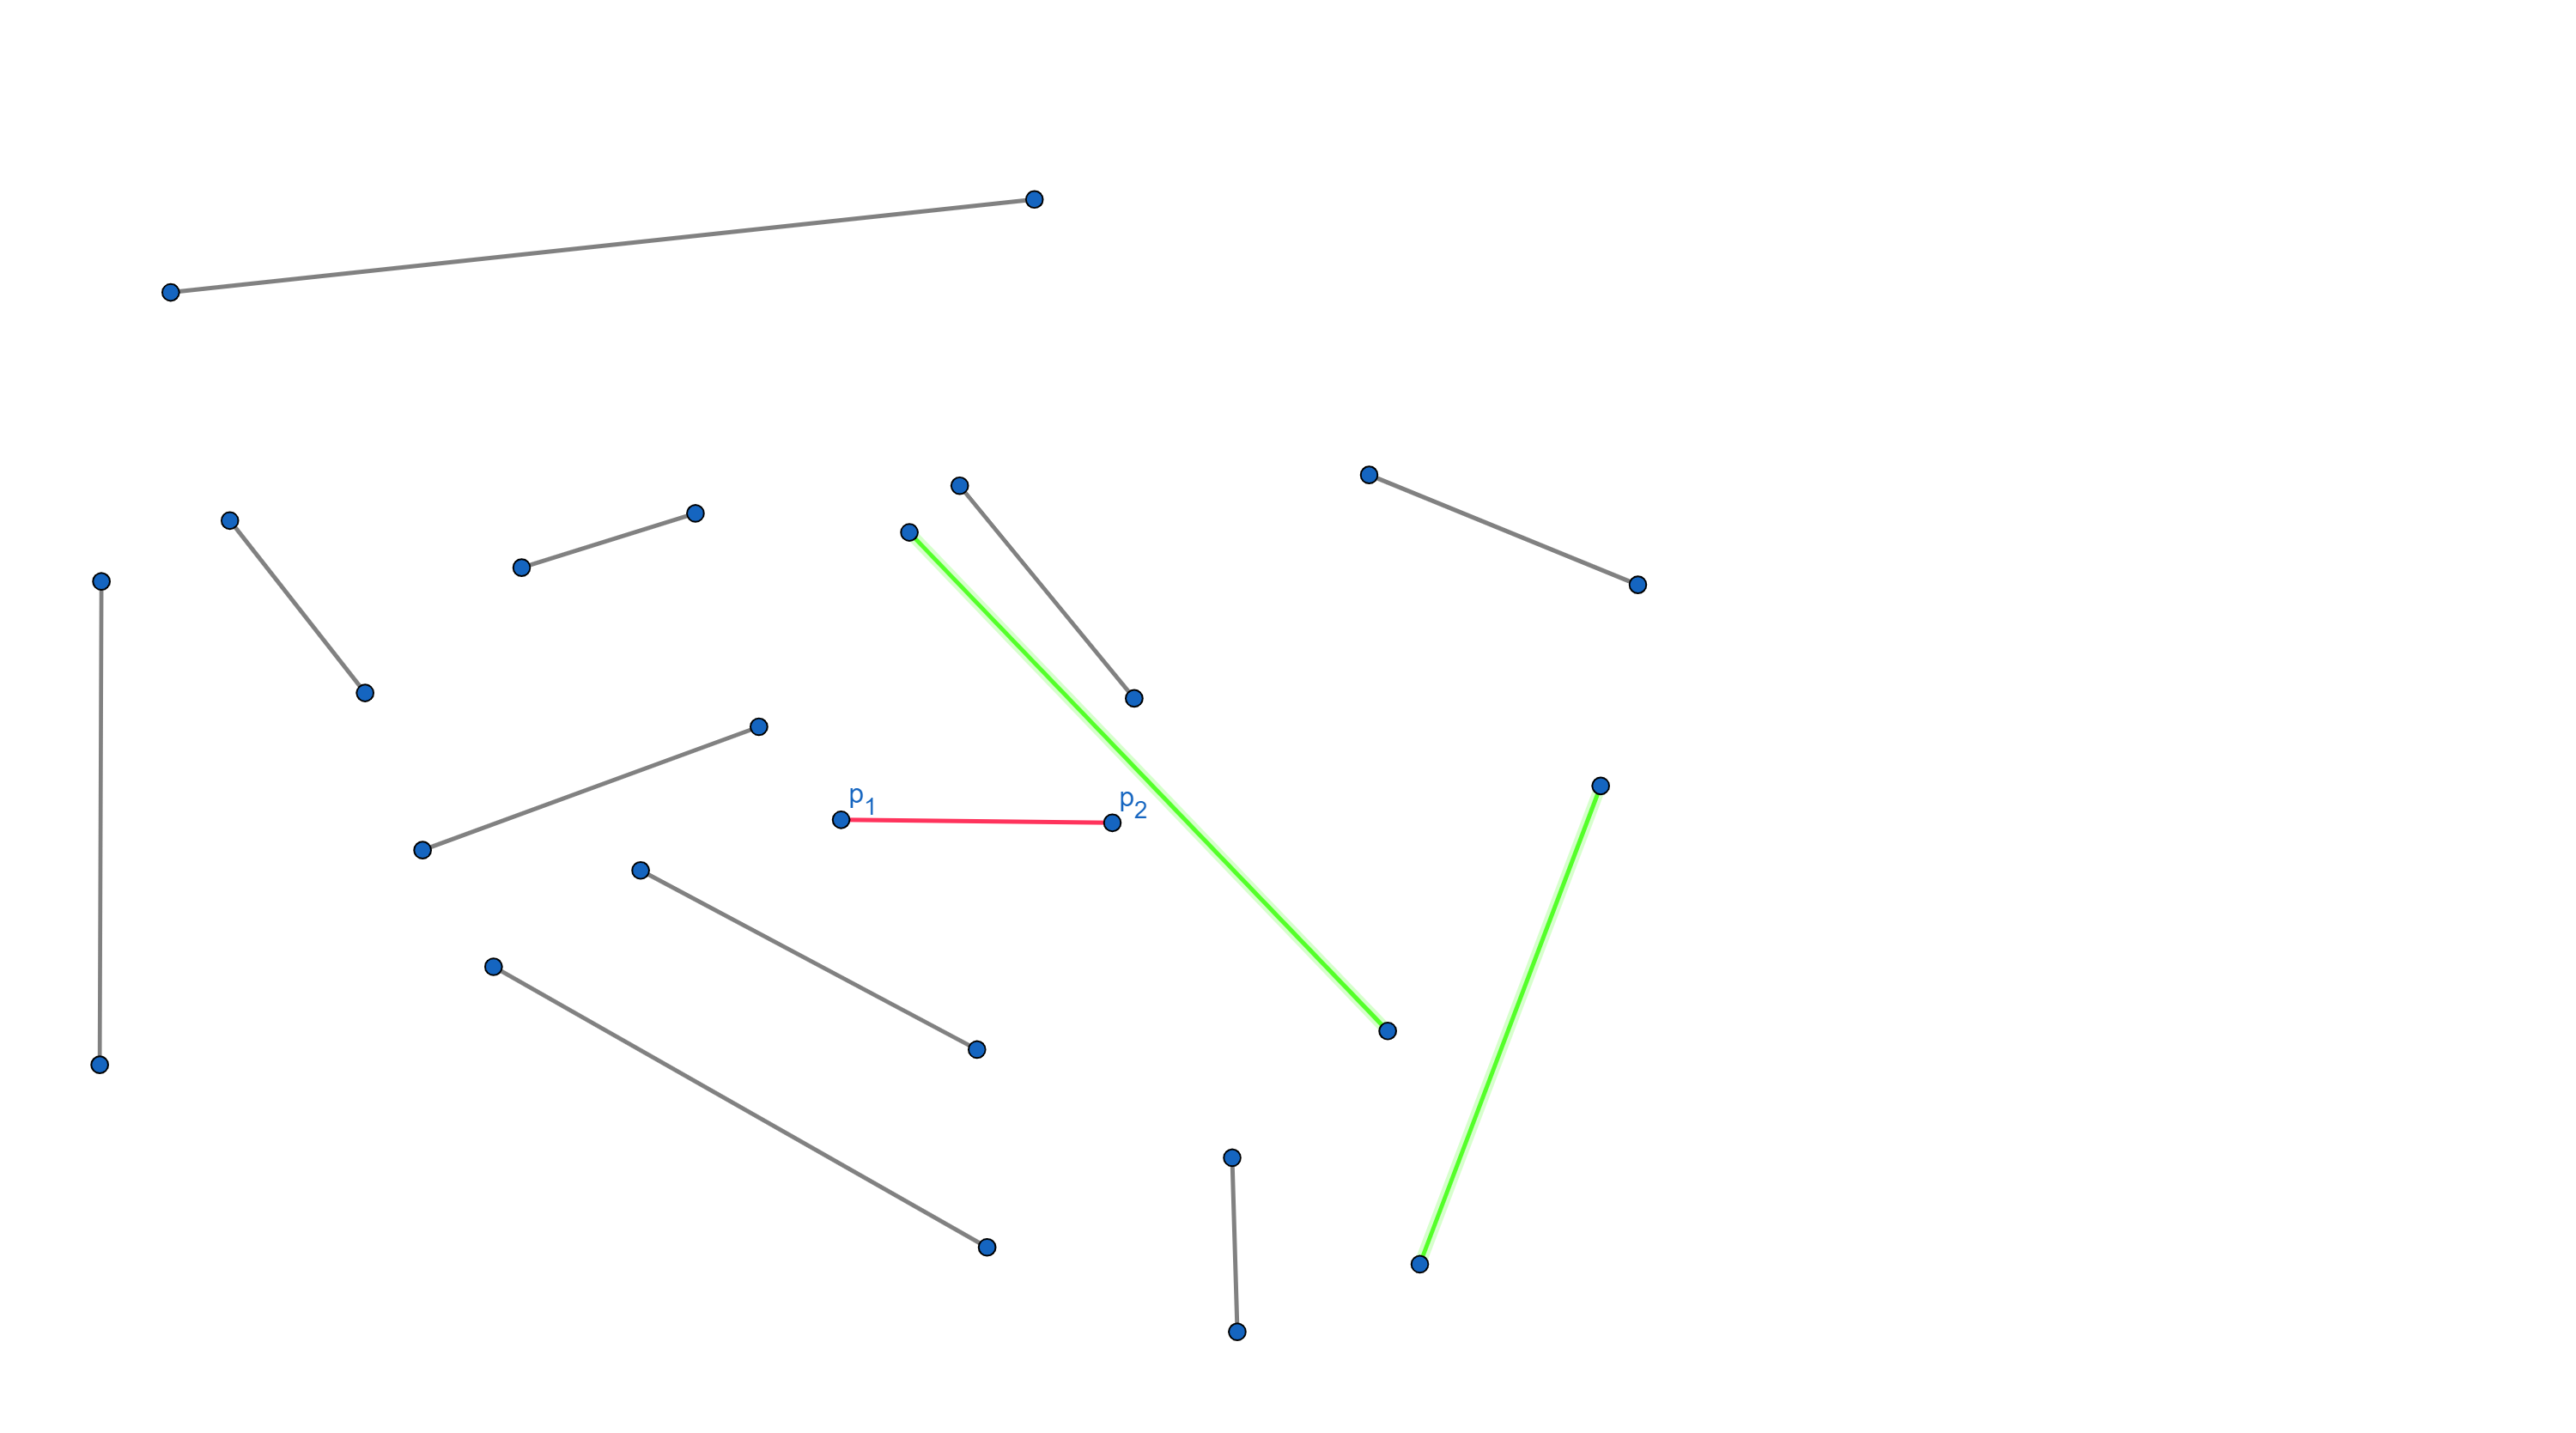
\includegraphics[width=0.5\linewidth]{segment_4.png}
            \end{figure}
            Любые другие прямые пересекали бы $p_1 p_2$ 
            (не допускаются).
\end{enumerate}
\par
Существование хотя бы одного отрезка в $S_1$ порождает
одну область <<нет-зоны>>, ограниченную двумя лучами и отрезком.
Для ее построения достаточно найти такие  $q_1, q_2 \in P_1$,
которые бы минимизировали углы $q_1 p_2 p_1$, $q_2 p_1 p_2$.
Далее строятся прямые на $q_1 p_2$ и $q_2 p_1$. Искомые лучи
лежат на полученных прямых, начинаются с $p_1$ и $p_2$, 
не включают $q_1$ и $q_2$.
\begin{figure}[H]
      \centering
      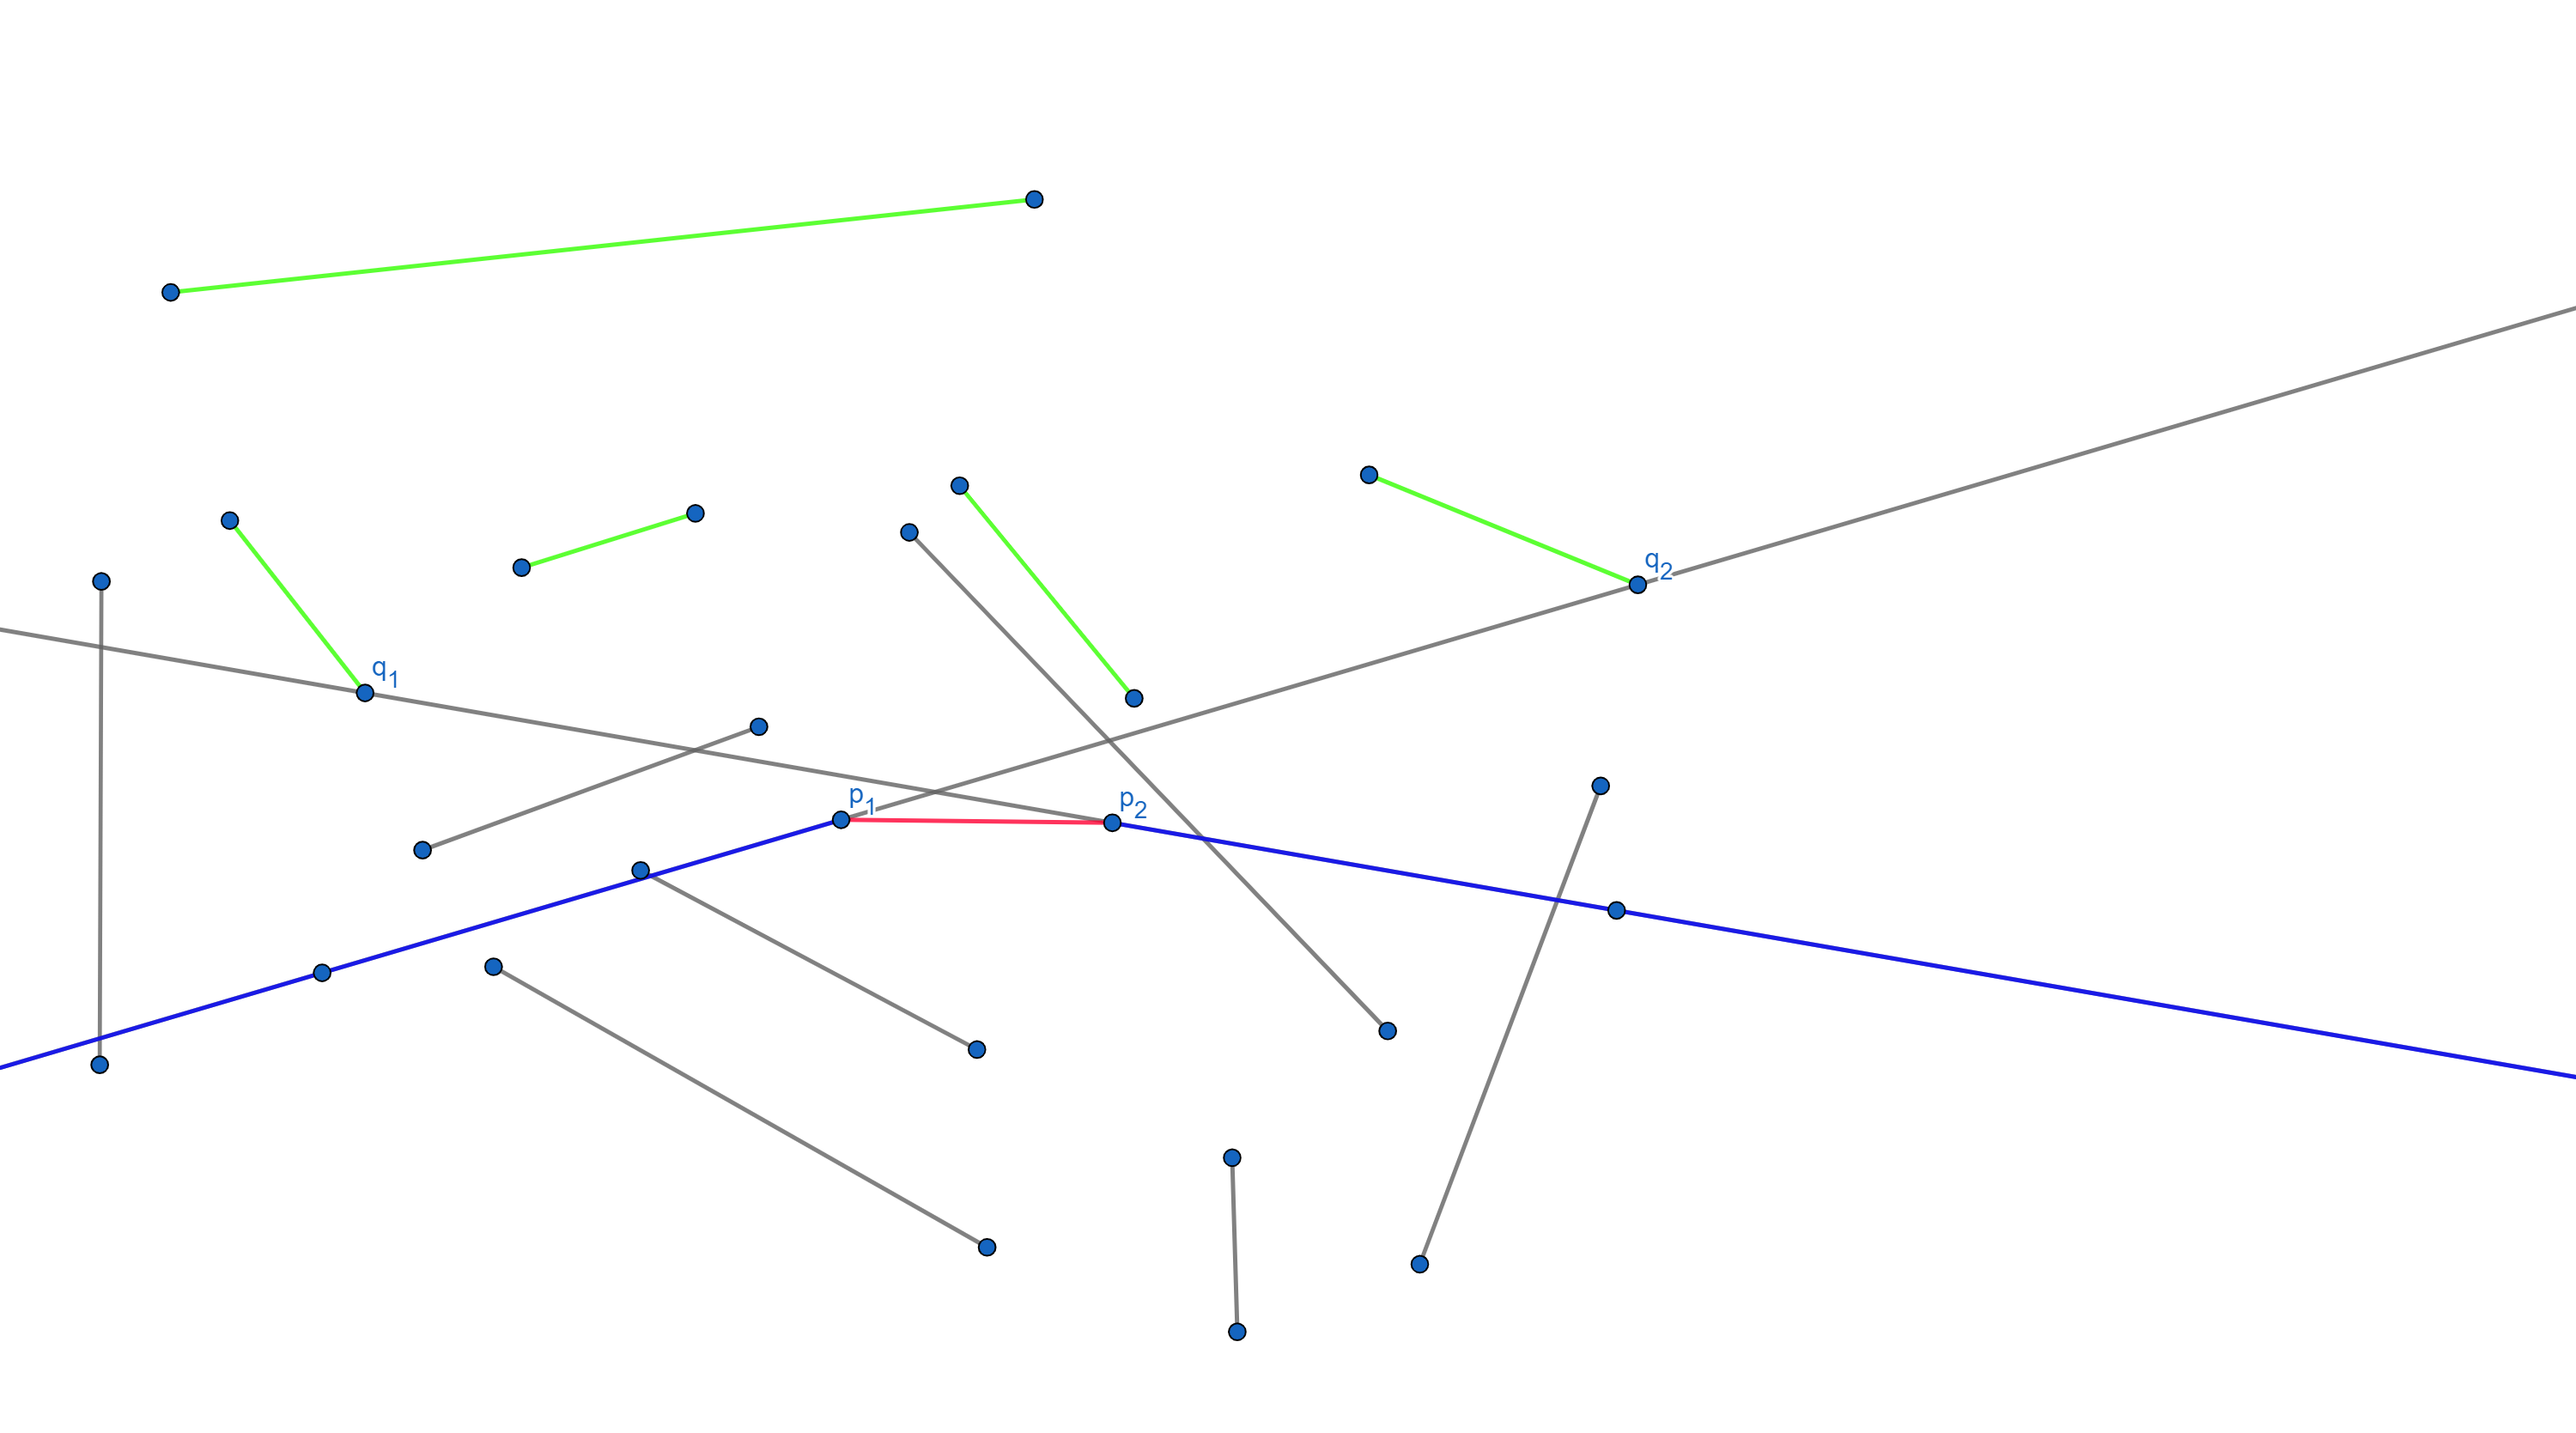
\includegraphics[width=0.5\linewidth]{rays_1.png}
\end{figure}
\par
Аналогично для $S_2$.
\begin{figure}[H]
      \centering
      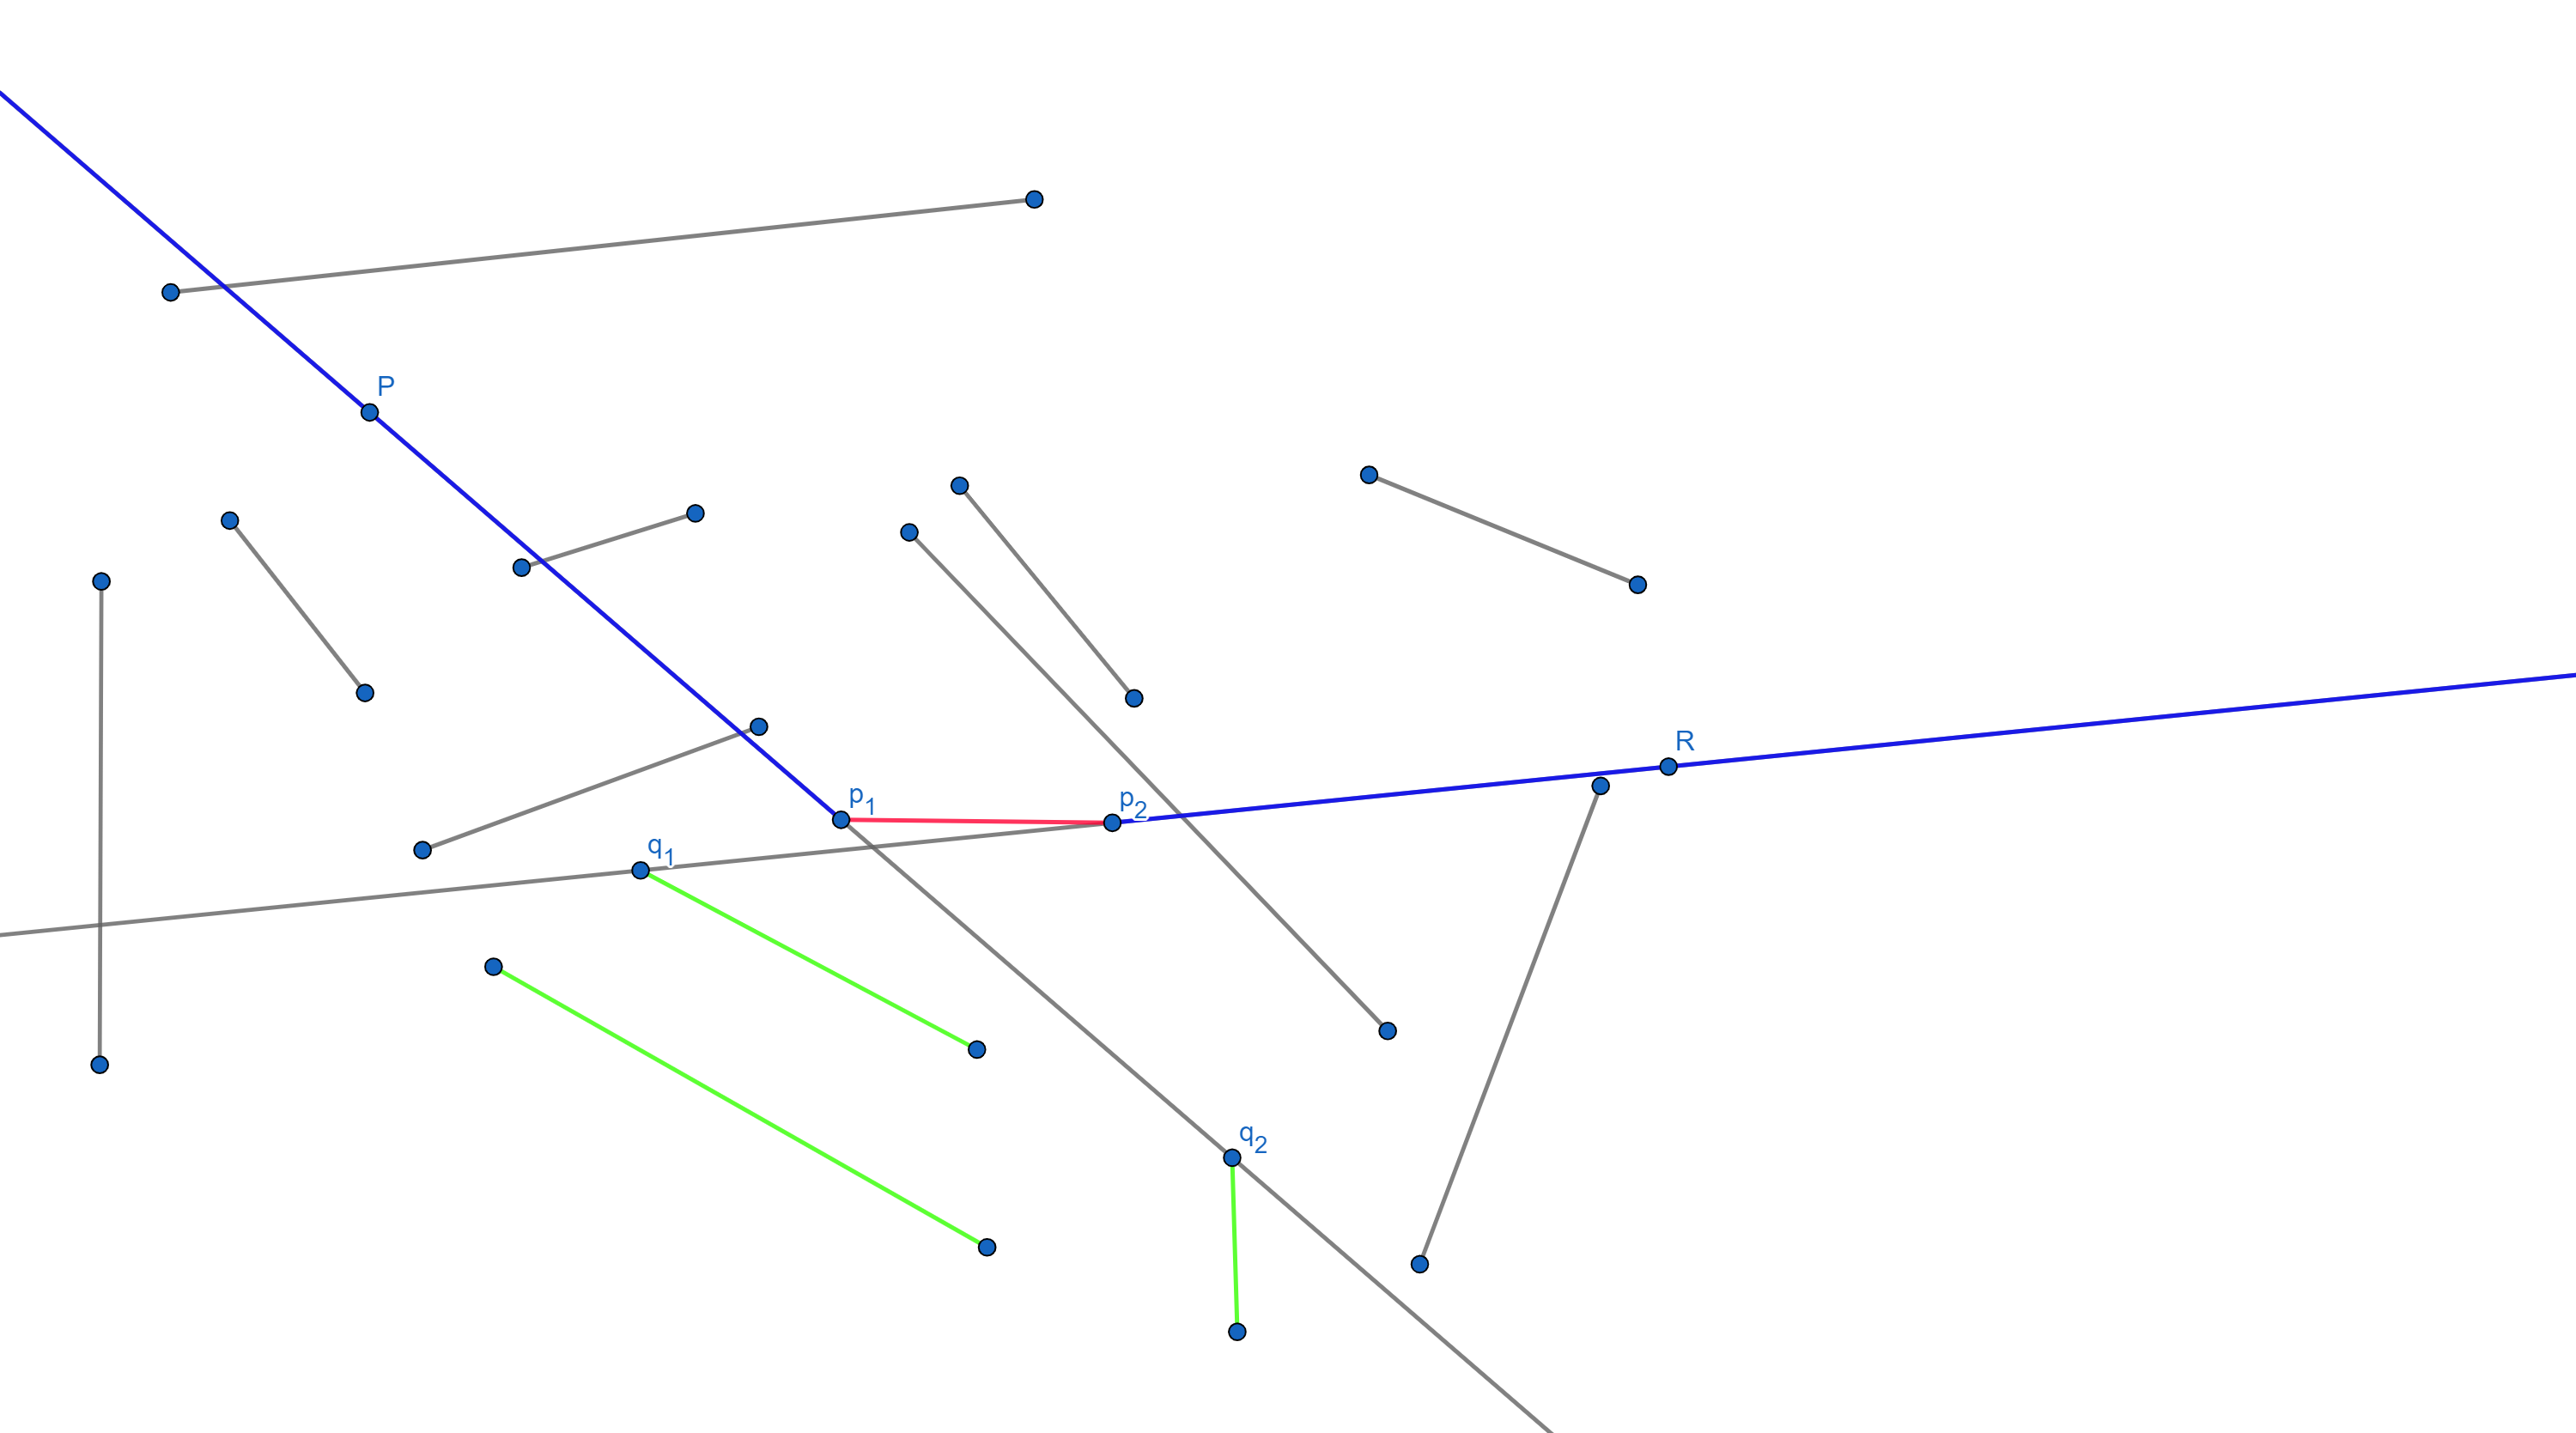
\includegraphics[width=0.5\linewidth]{rays_2.png}
\end{figure}
\par
Существование хотя бы одного отрезка в $S_3$ также порождает
одну область <<нет-зоны>>, ограниченную двумя лучами.
Для ее построения достаточно найти такие  $q_1, q_2 \in P_3$,
которые бы минимизировали углы $q_1 p_1 p_2$, $q_2 p_1 p_2$
при условии того, что $q_1$ лежит левее $p_1 p_2$, а $q_1$
правее. Далее строятся прямые на $q_1 p_1$ и $q_2 p_1$. 
Искомые лучи лежат на полученных прямых, начинаются с 
$p_1$, не включают $q_1$ и $q_2$.
\begin{figure}[H]
      \centering
      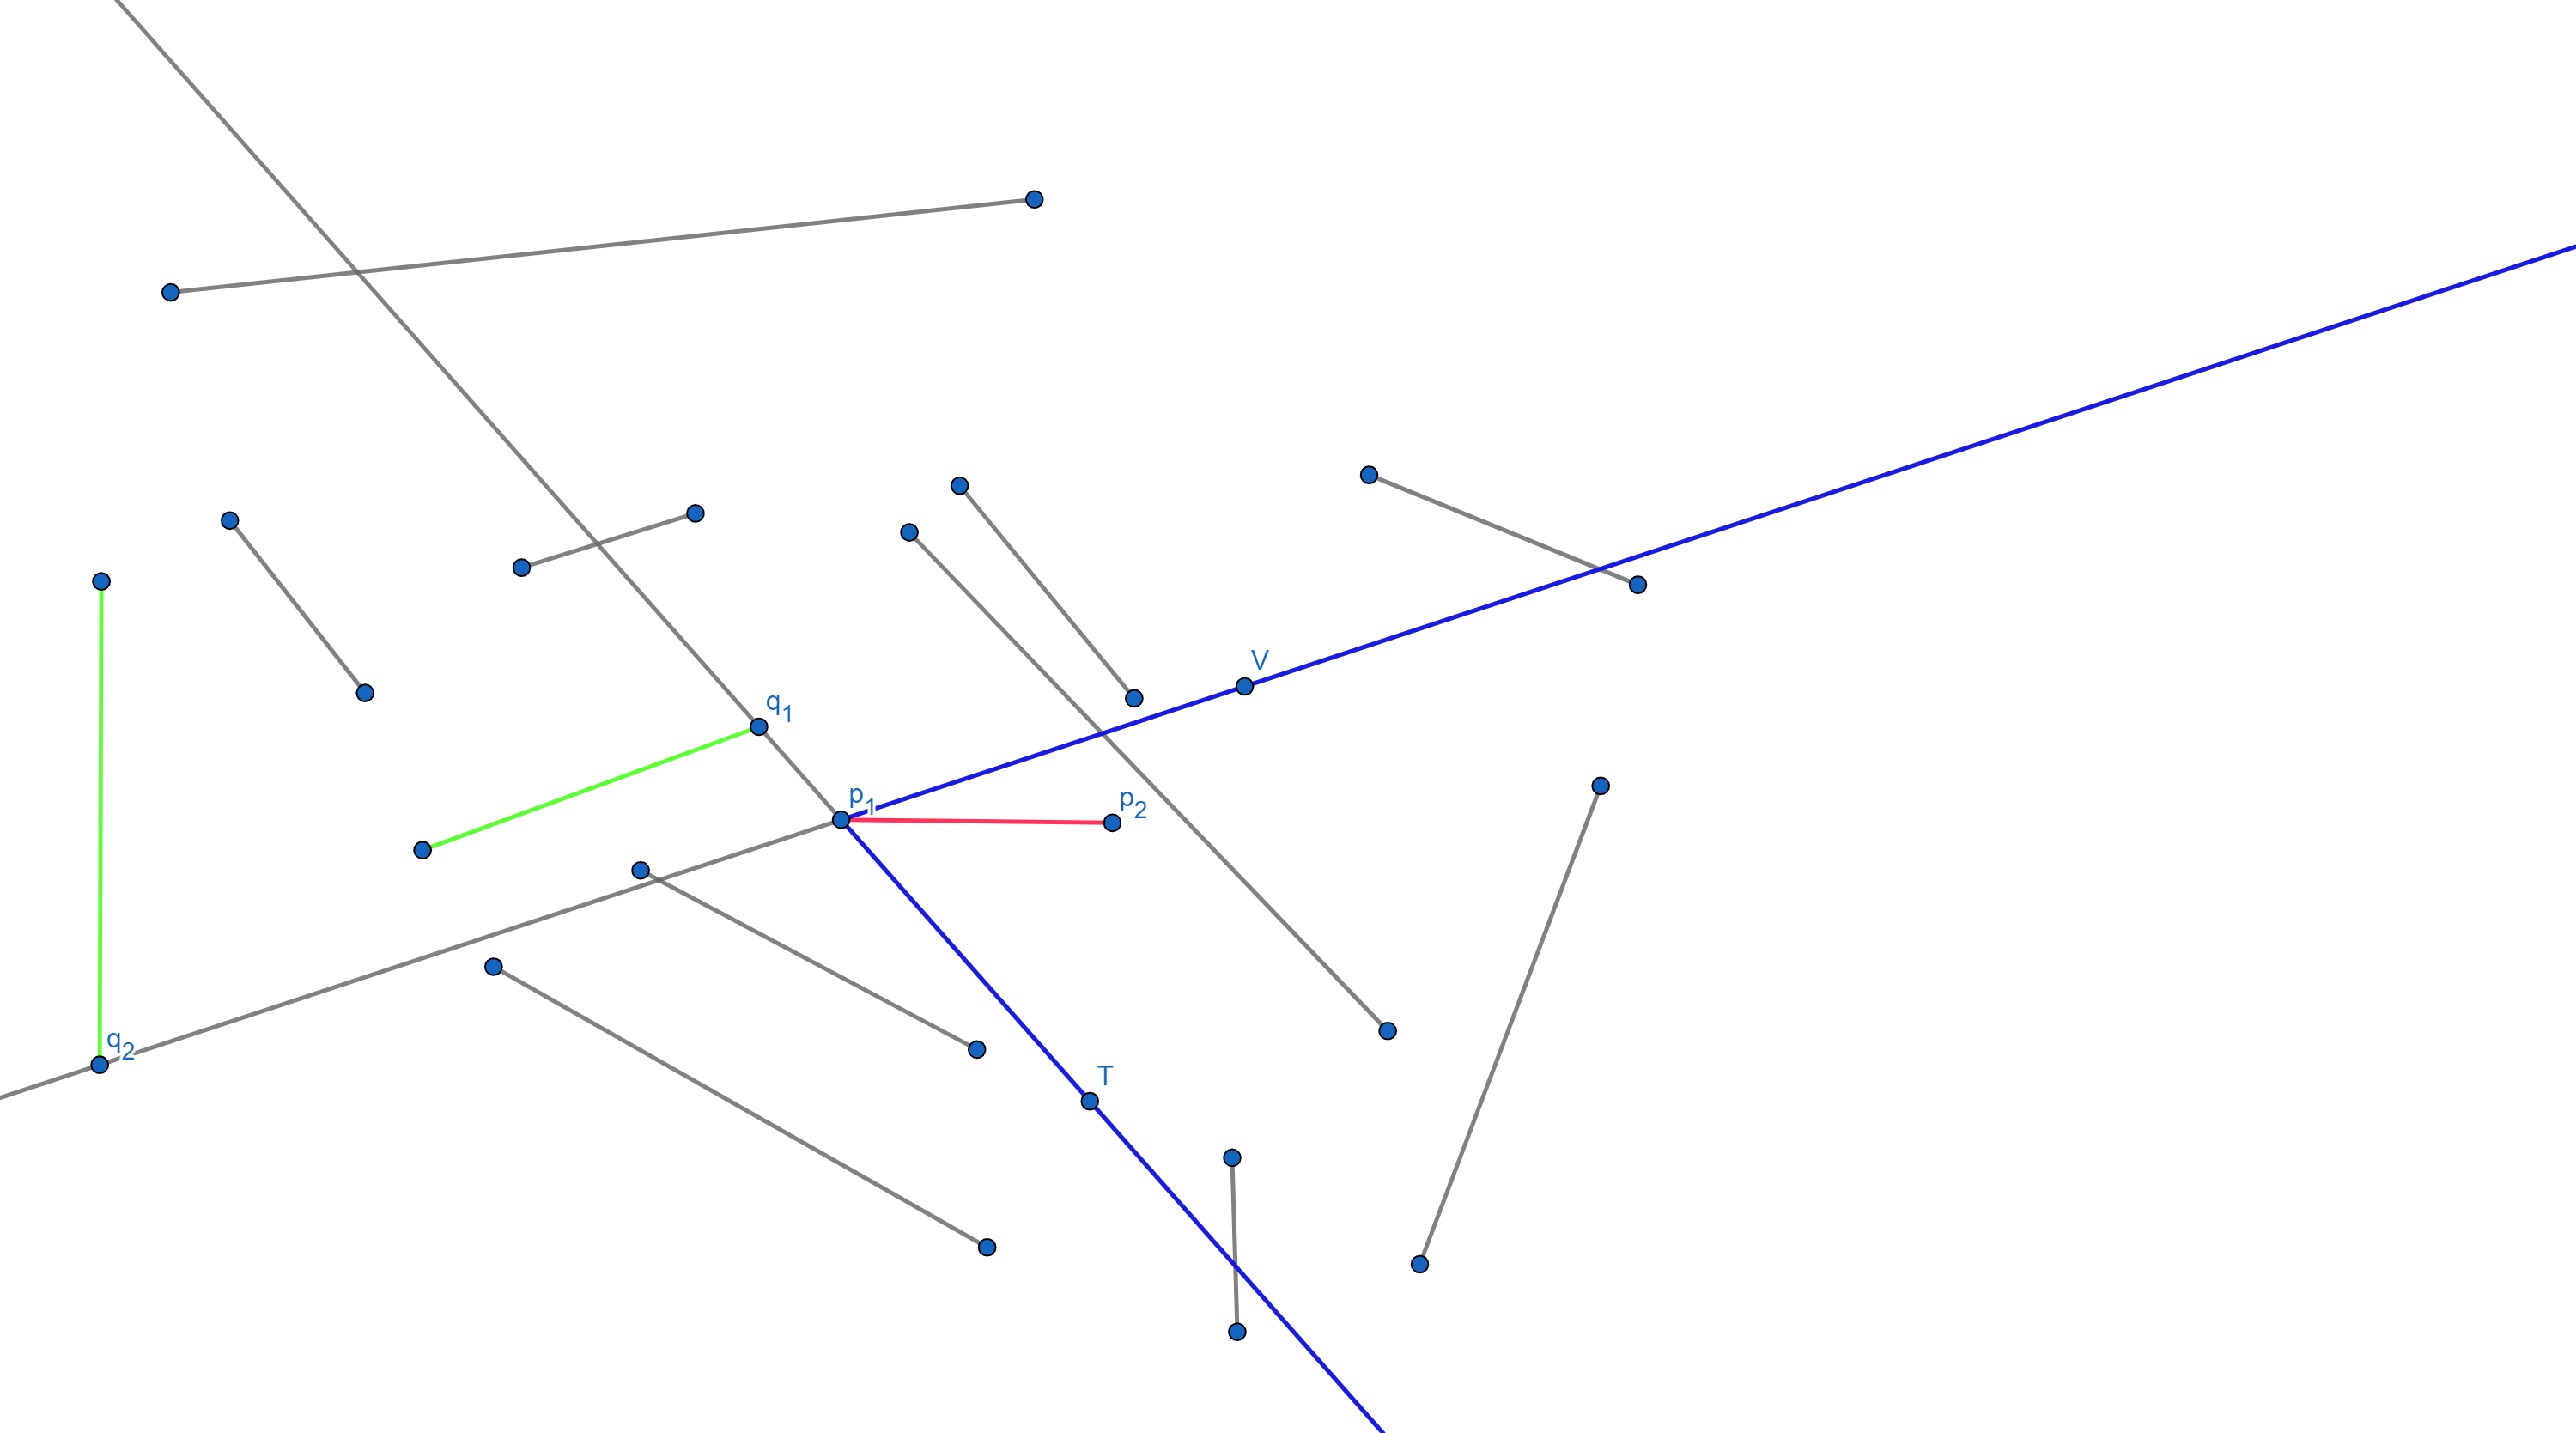
\includegraphics[width=0.5\linewidth]{rays_3.png}
\end{figure}
\par
Для $S_4$ минимизируются углы $q_1 p_2 p_1$, $q_2 p_2 p_1$,
лучи начинаются с $p_2$.
\begin{figure}[H]
      \centering
      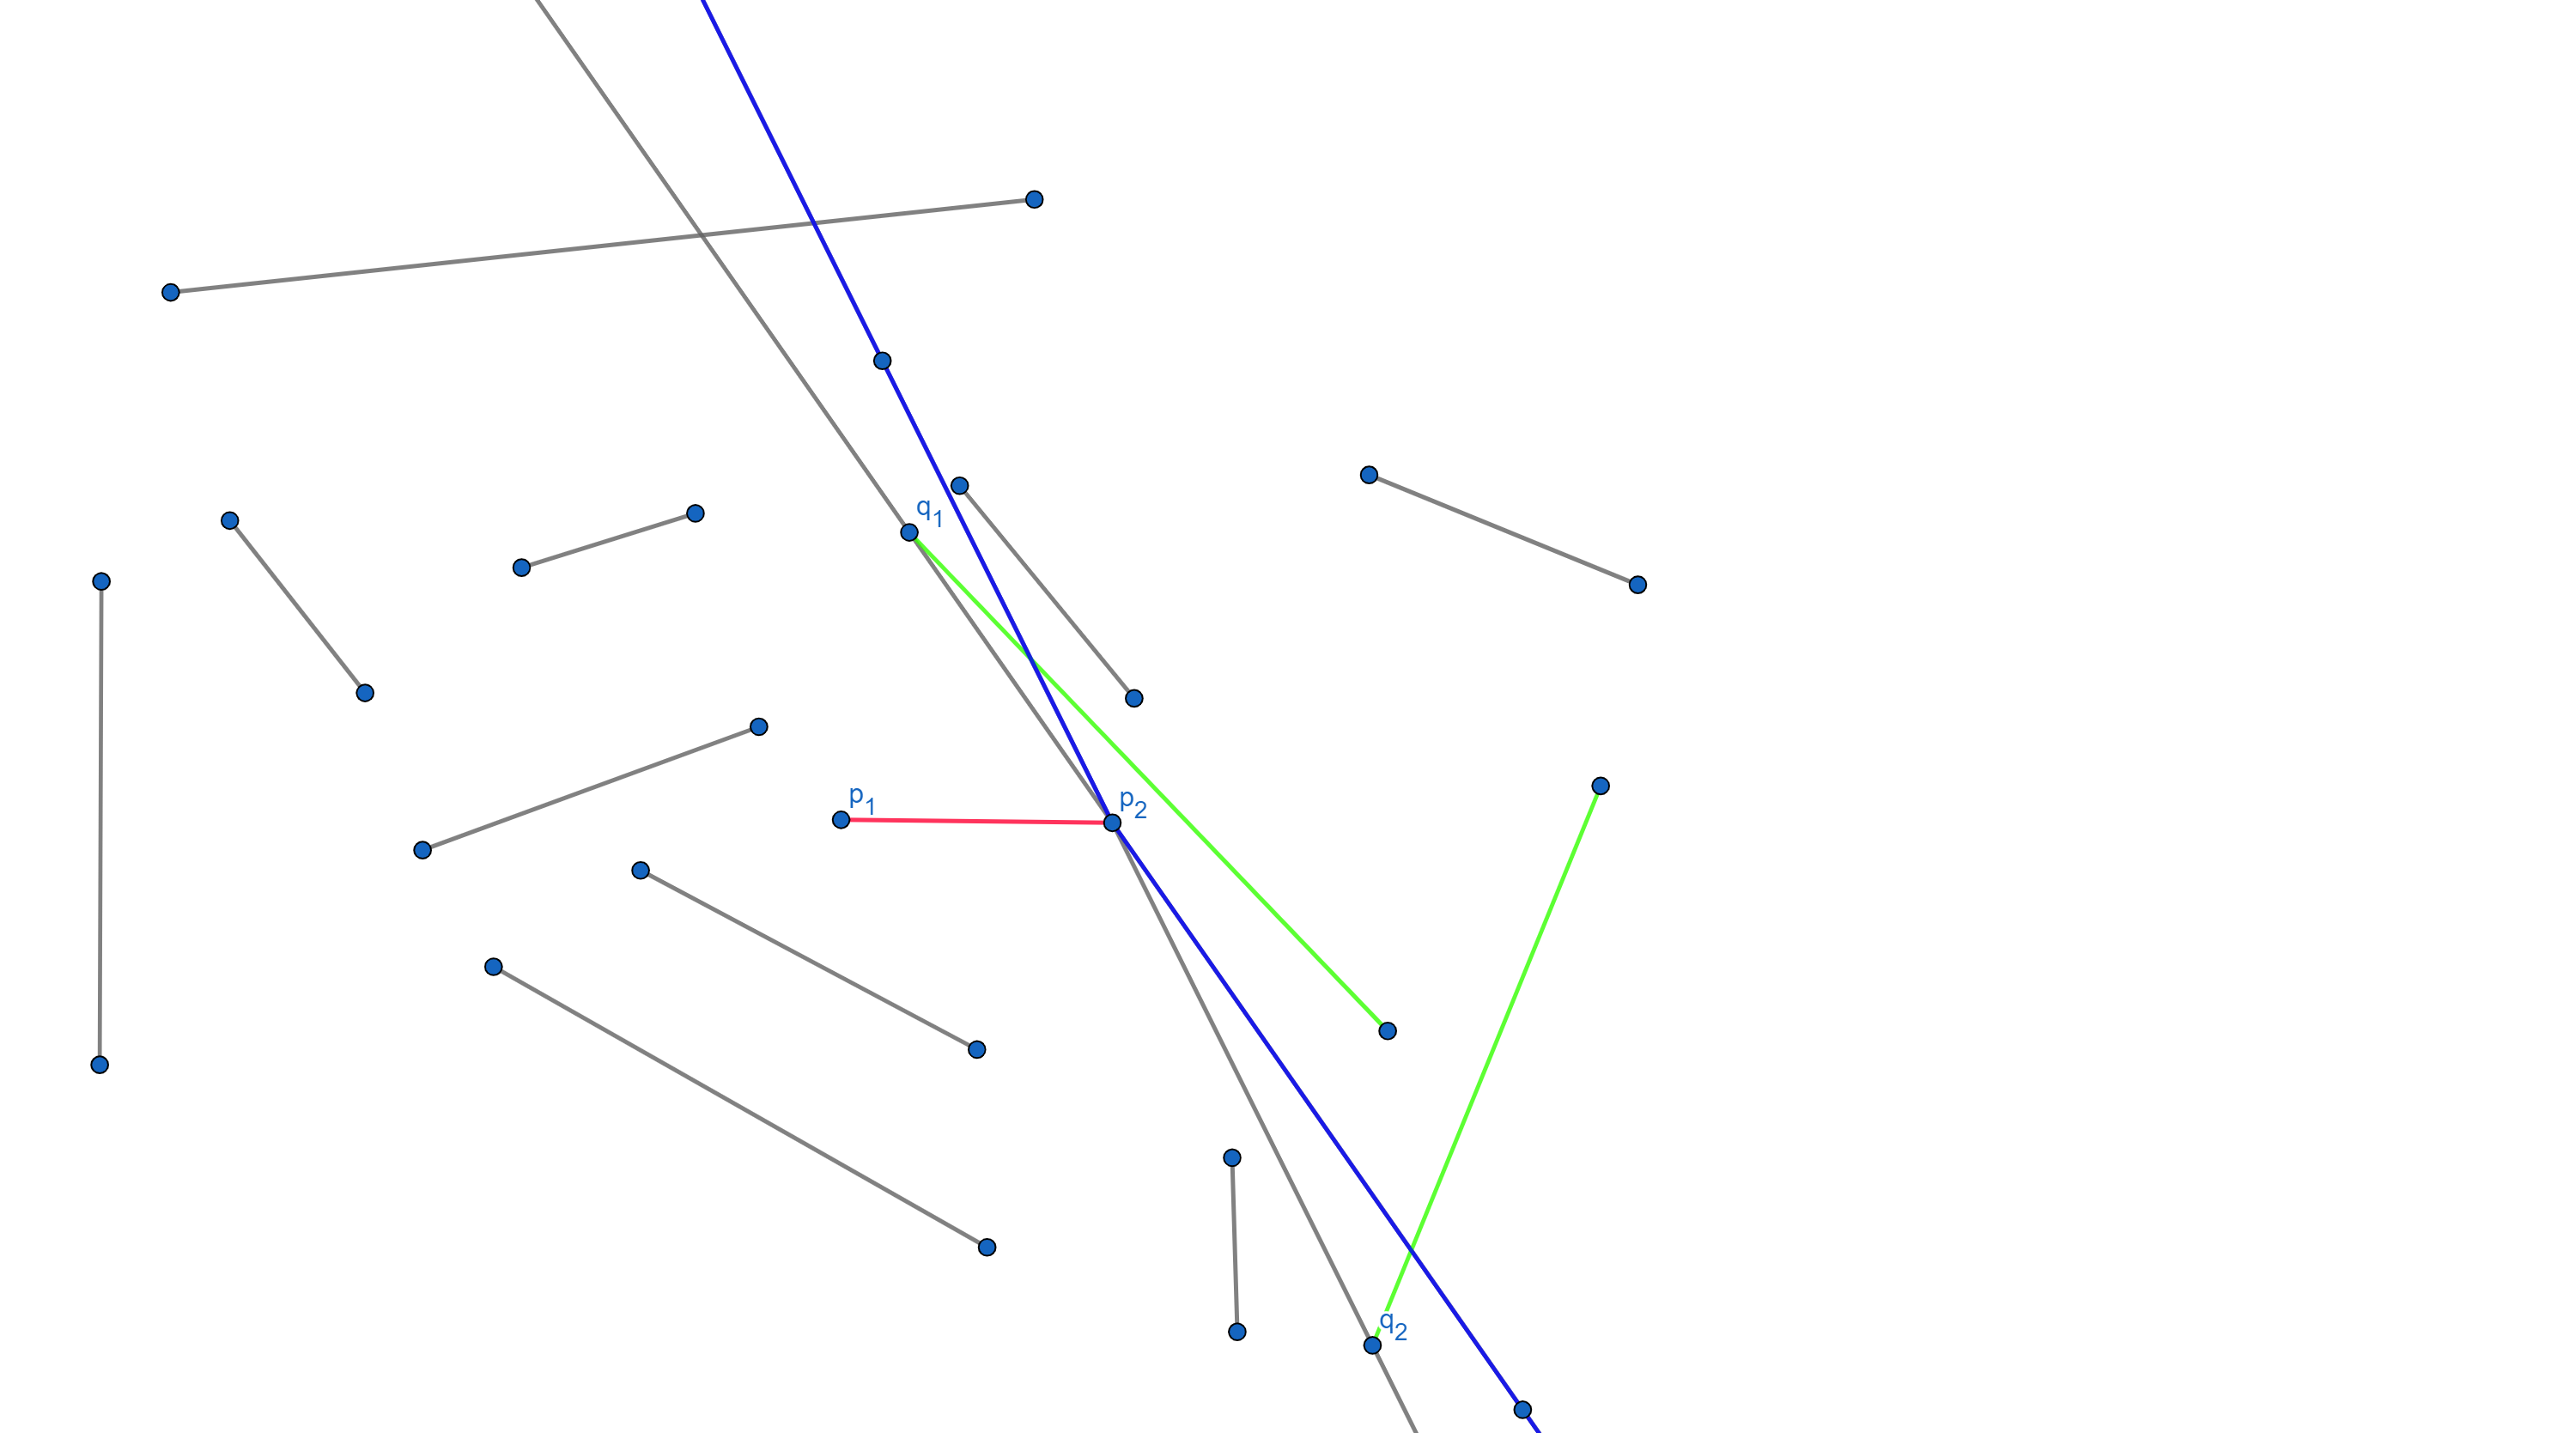
\includegraphics[width=0.5\linewidth]{rays_4.png}
\end{figure}
\par
Таким образом, $S_1$ порождает <<нет-зону>>: 
луч-$p_1 p_2$-луч. Причем лучи непересекающиеся, 
%Кажется даже параллельными быть не могут?
а зона -- подмножество полуплоскости. %Включение строгое
Аналогично для $S_2$.
\par
$S_3$ порождает <<нет-зону>>: луч-$p_1$-луч. 
Вырожденной зона быть не может, если непусто $S_3$.
Данная зона может быть сколь угодно близкой как к прямой,
так и ко всей плоскости.
Аналогично для $S_4$.
\par
Итоговая <<нет-зона>> получается пересечением полученных выше.
Для данного примера она получается равной всей плоскости, а
значит мы получаем досрочный ответ <<нет>> для задачи видимости.
\par
Все виды итоговых <<нет-зон>> можно получить перебором:
\begin{enumerate}
      \item Зоны, порождаемые $S_1$ и $S_2$, непересекаются, 
            так что результат всегда один: множество, 
            ограниченное конструкциями луч-$p_1$-луч, 
            луч-$p_2$-луч.
            \begin{figure}[H]
                  \centering
                  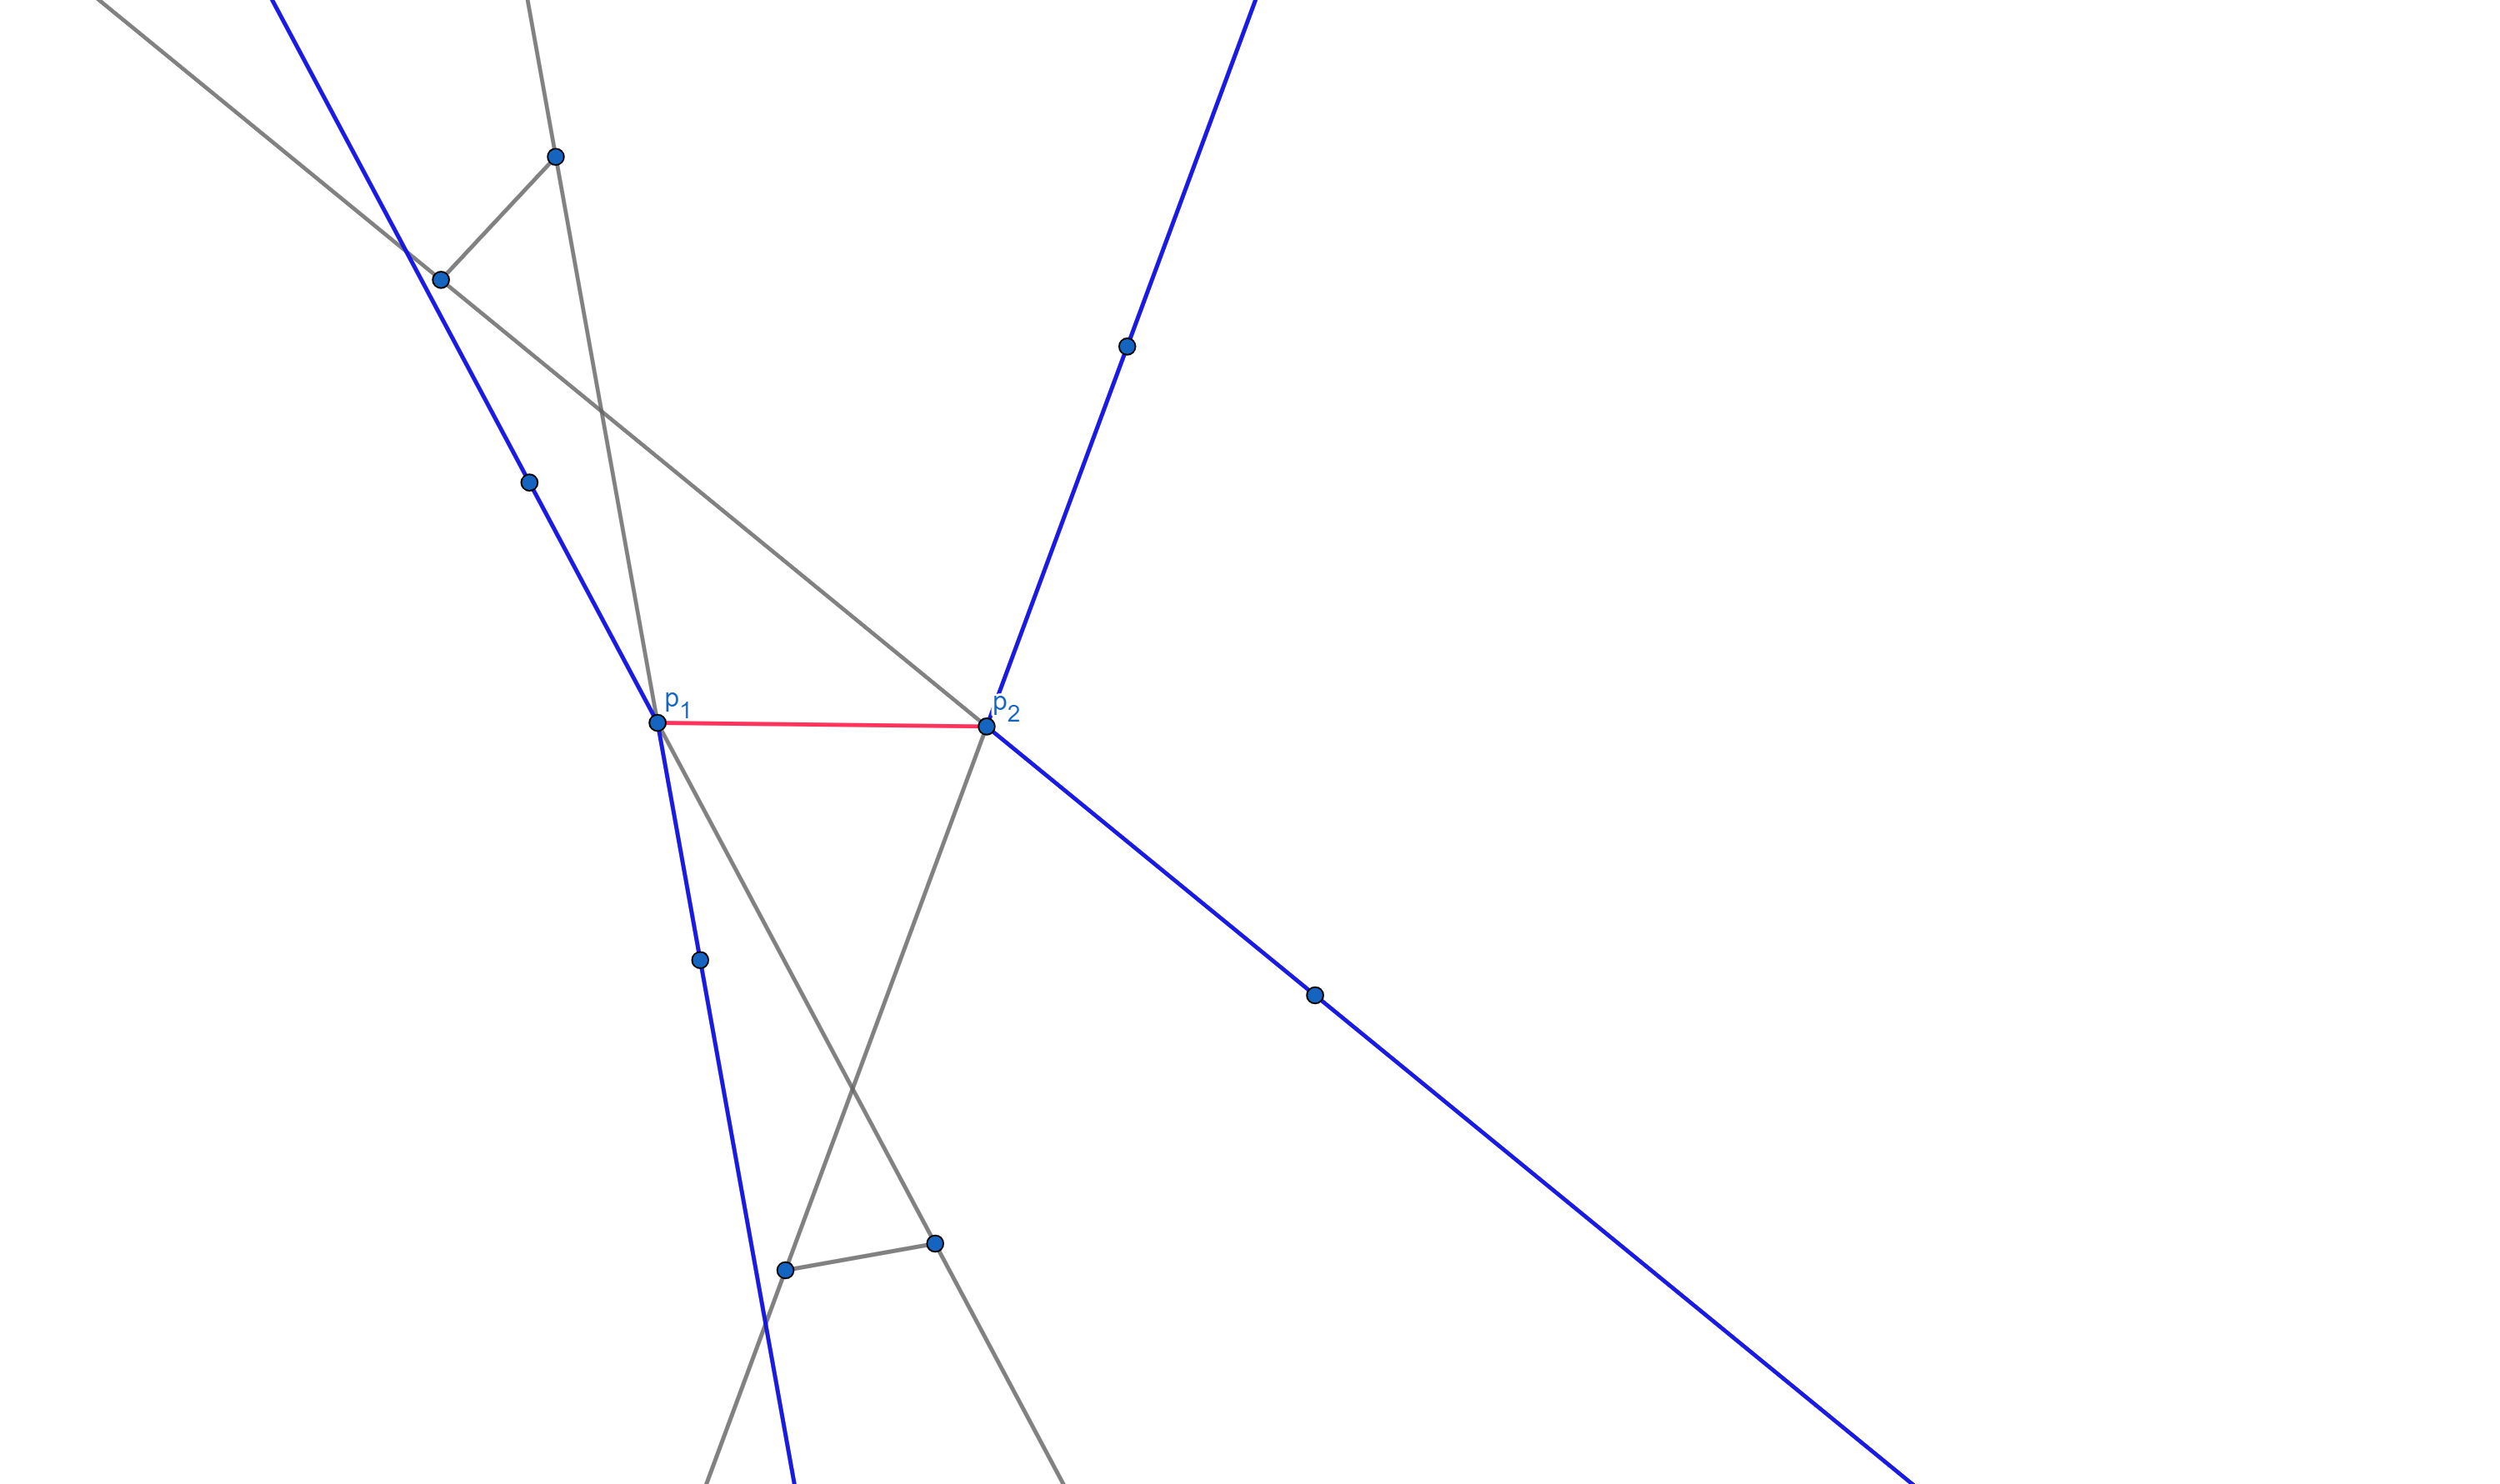
\includegraphics[width=0.5\linewidth]{nozone_2_1.png}
            \end{figure}
      \item Взаимодействие зон, порождаемых $S_3$ и $S_4$, 
            можно поделить на взаимодействие левых и правых
            лучей. Одни из них всегда пересекаются (обозначим
            точку пекресечения $k_1$). В этой полуплоскости
            итоговая зона ограничена конструкцией
            луч-$k_1$-луч. Во второй полуплоскости возможны два
            варианта: пересечение лучей в точке $k_2$ или
            отсутсвие пересечения. Итого результат: множество, 
            ограниченное либо конструкциями луч-$k_1$-луч, 
            луч-$k_2$-луч, либо только луч-$k_1$-луч.
            \begin{figure}[H]
                  \centering
                  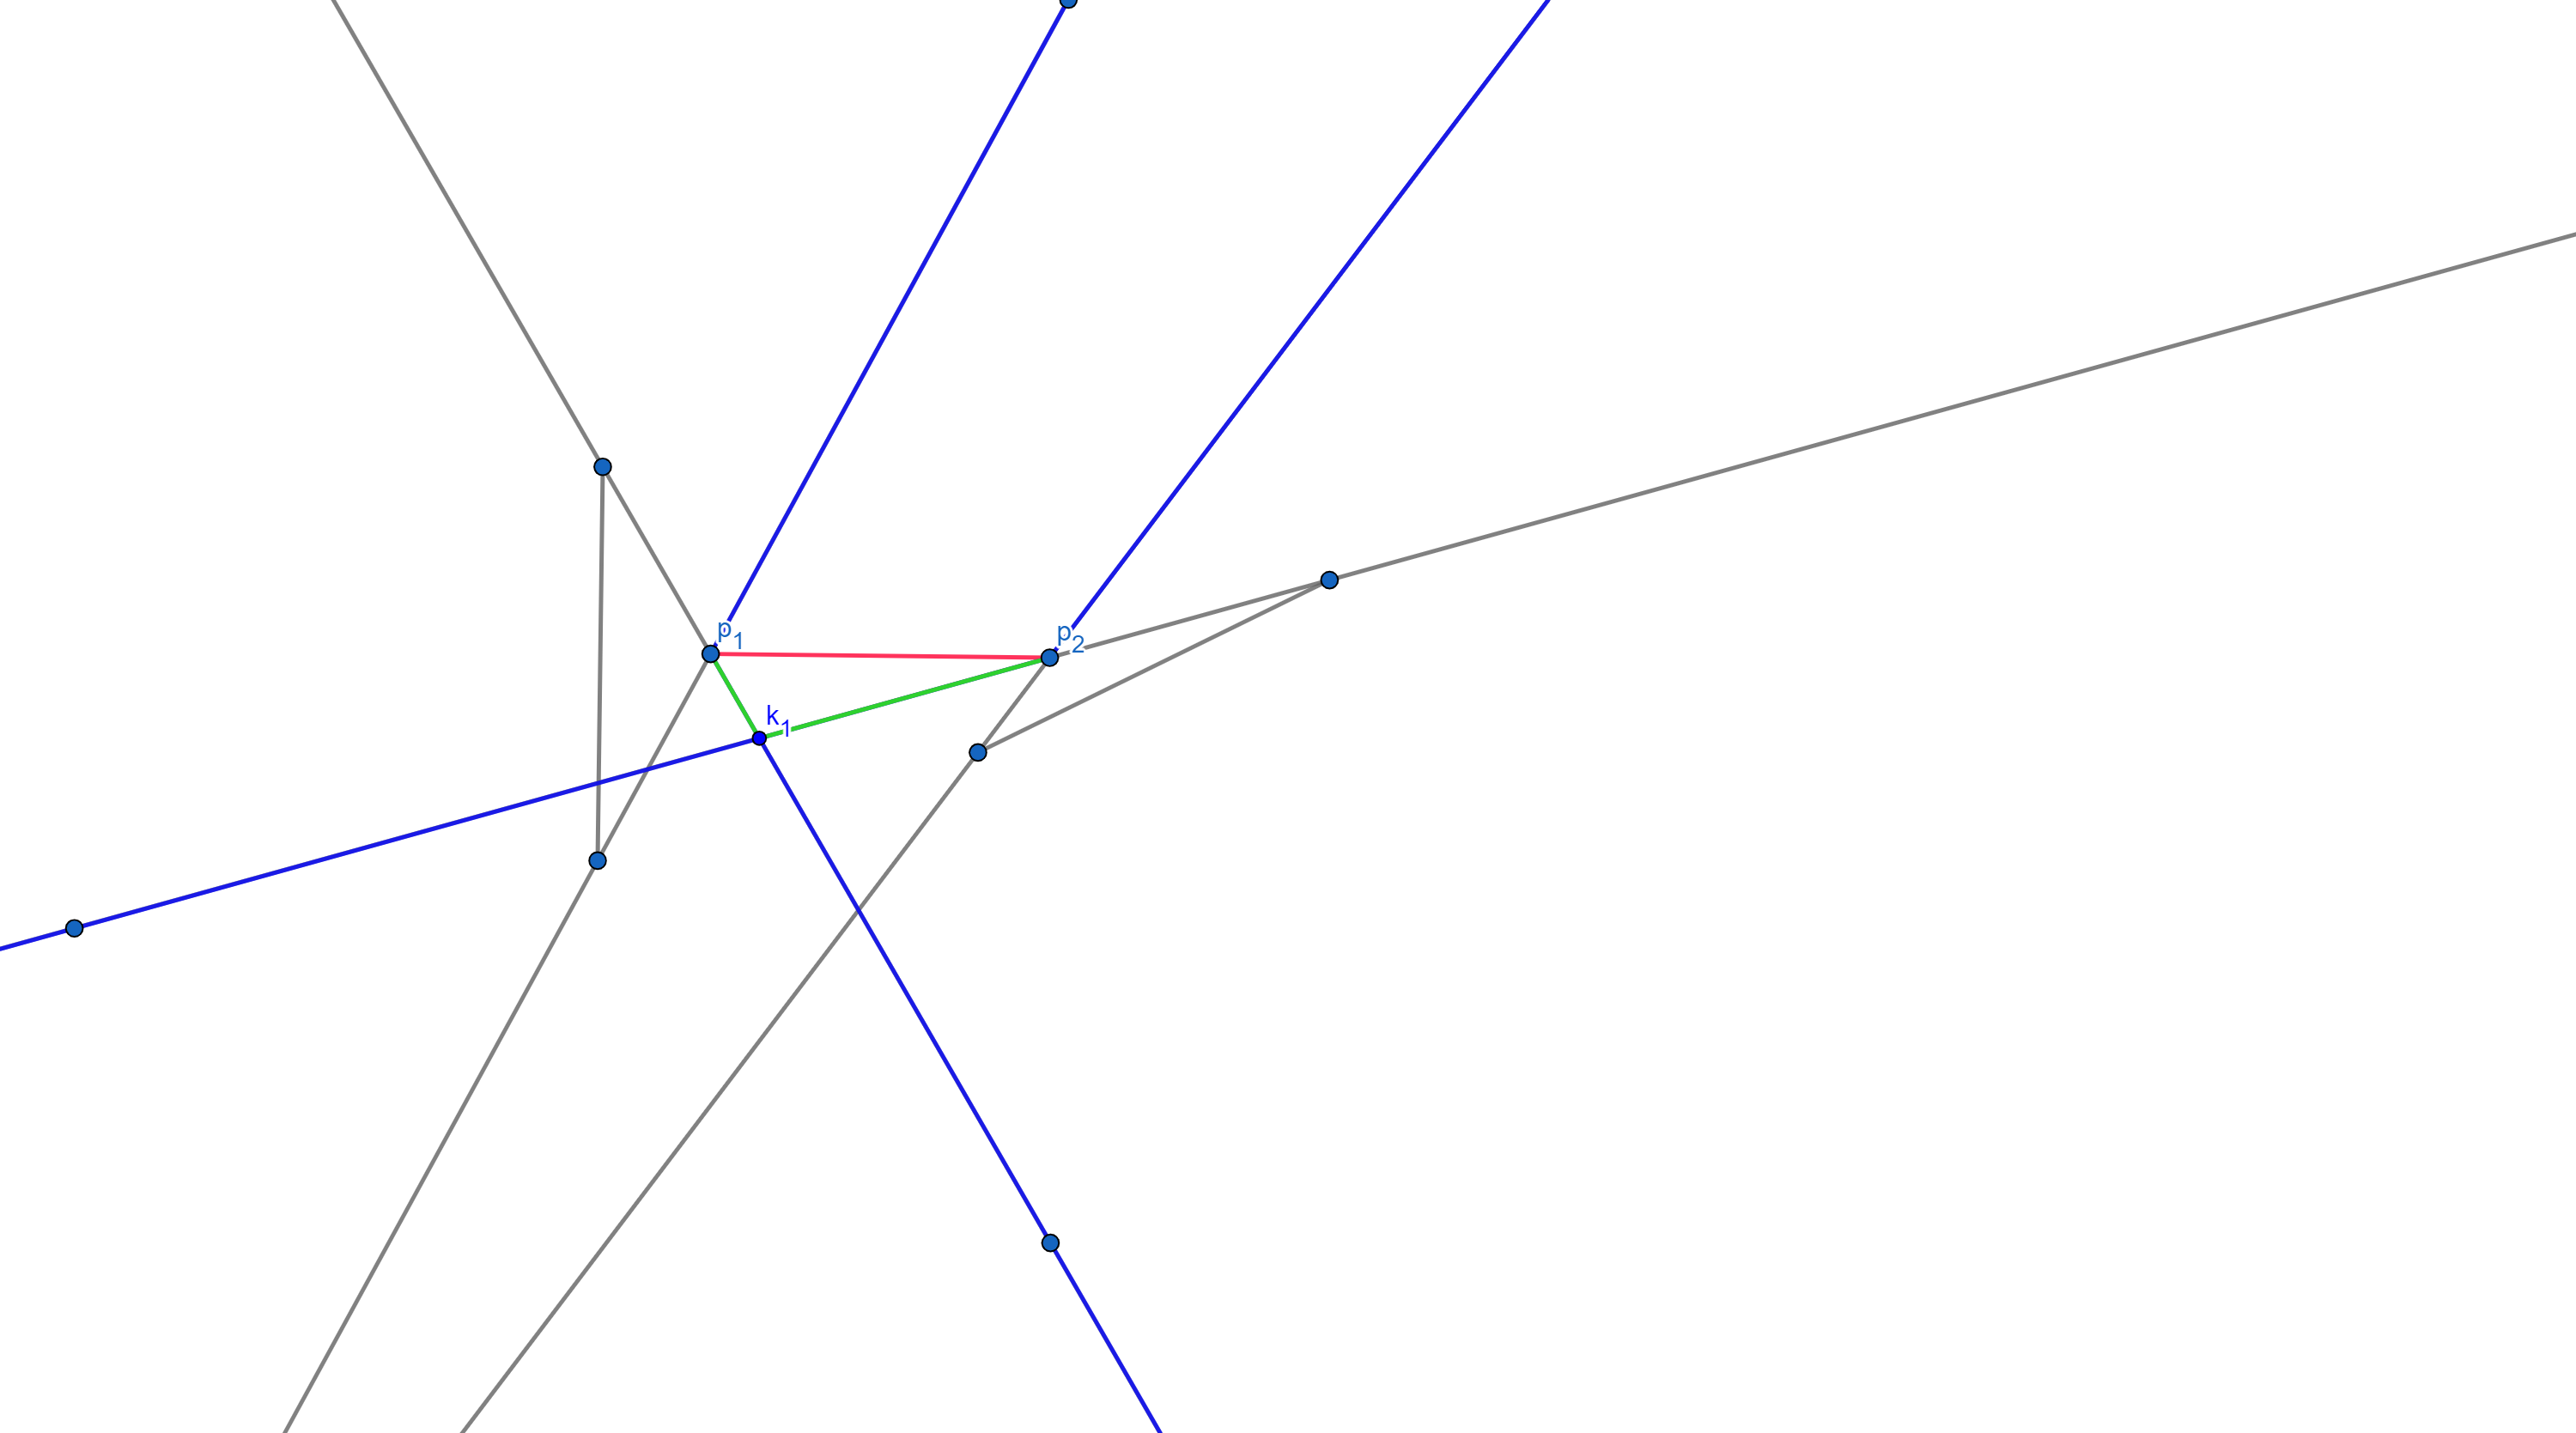
\includegraphics[width=0.5\linewidth]{nozone_2_2.png}
            \end{figure}
            \begin{figure}[H]
                  \centering
                  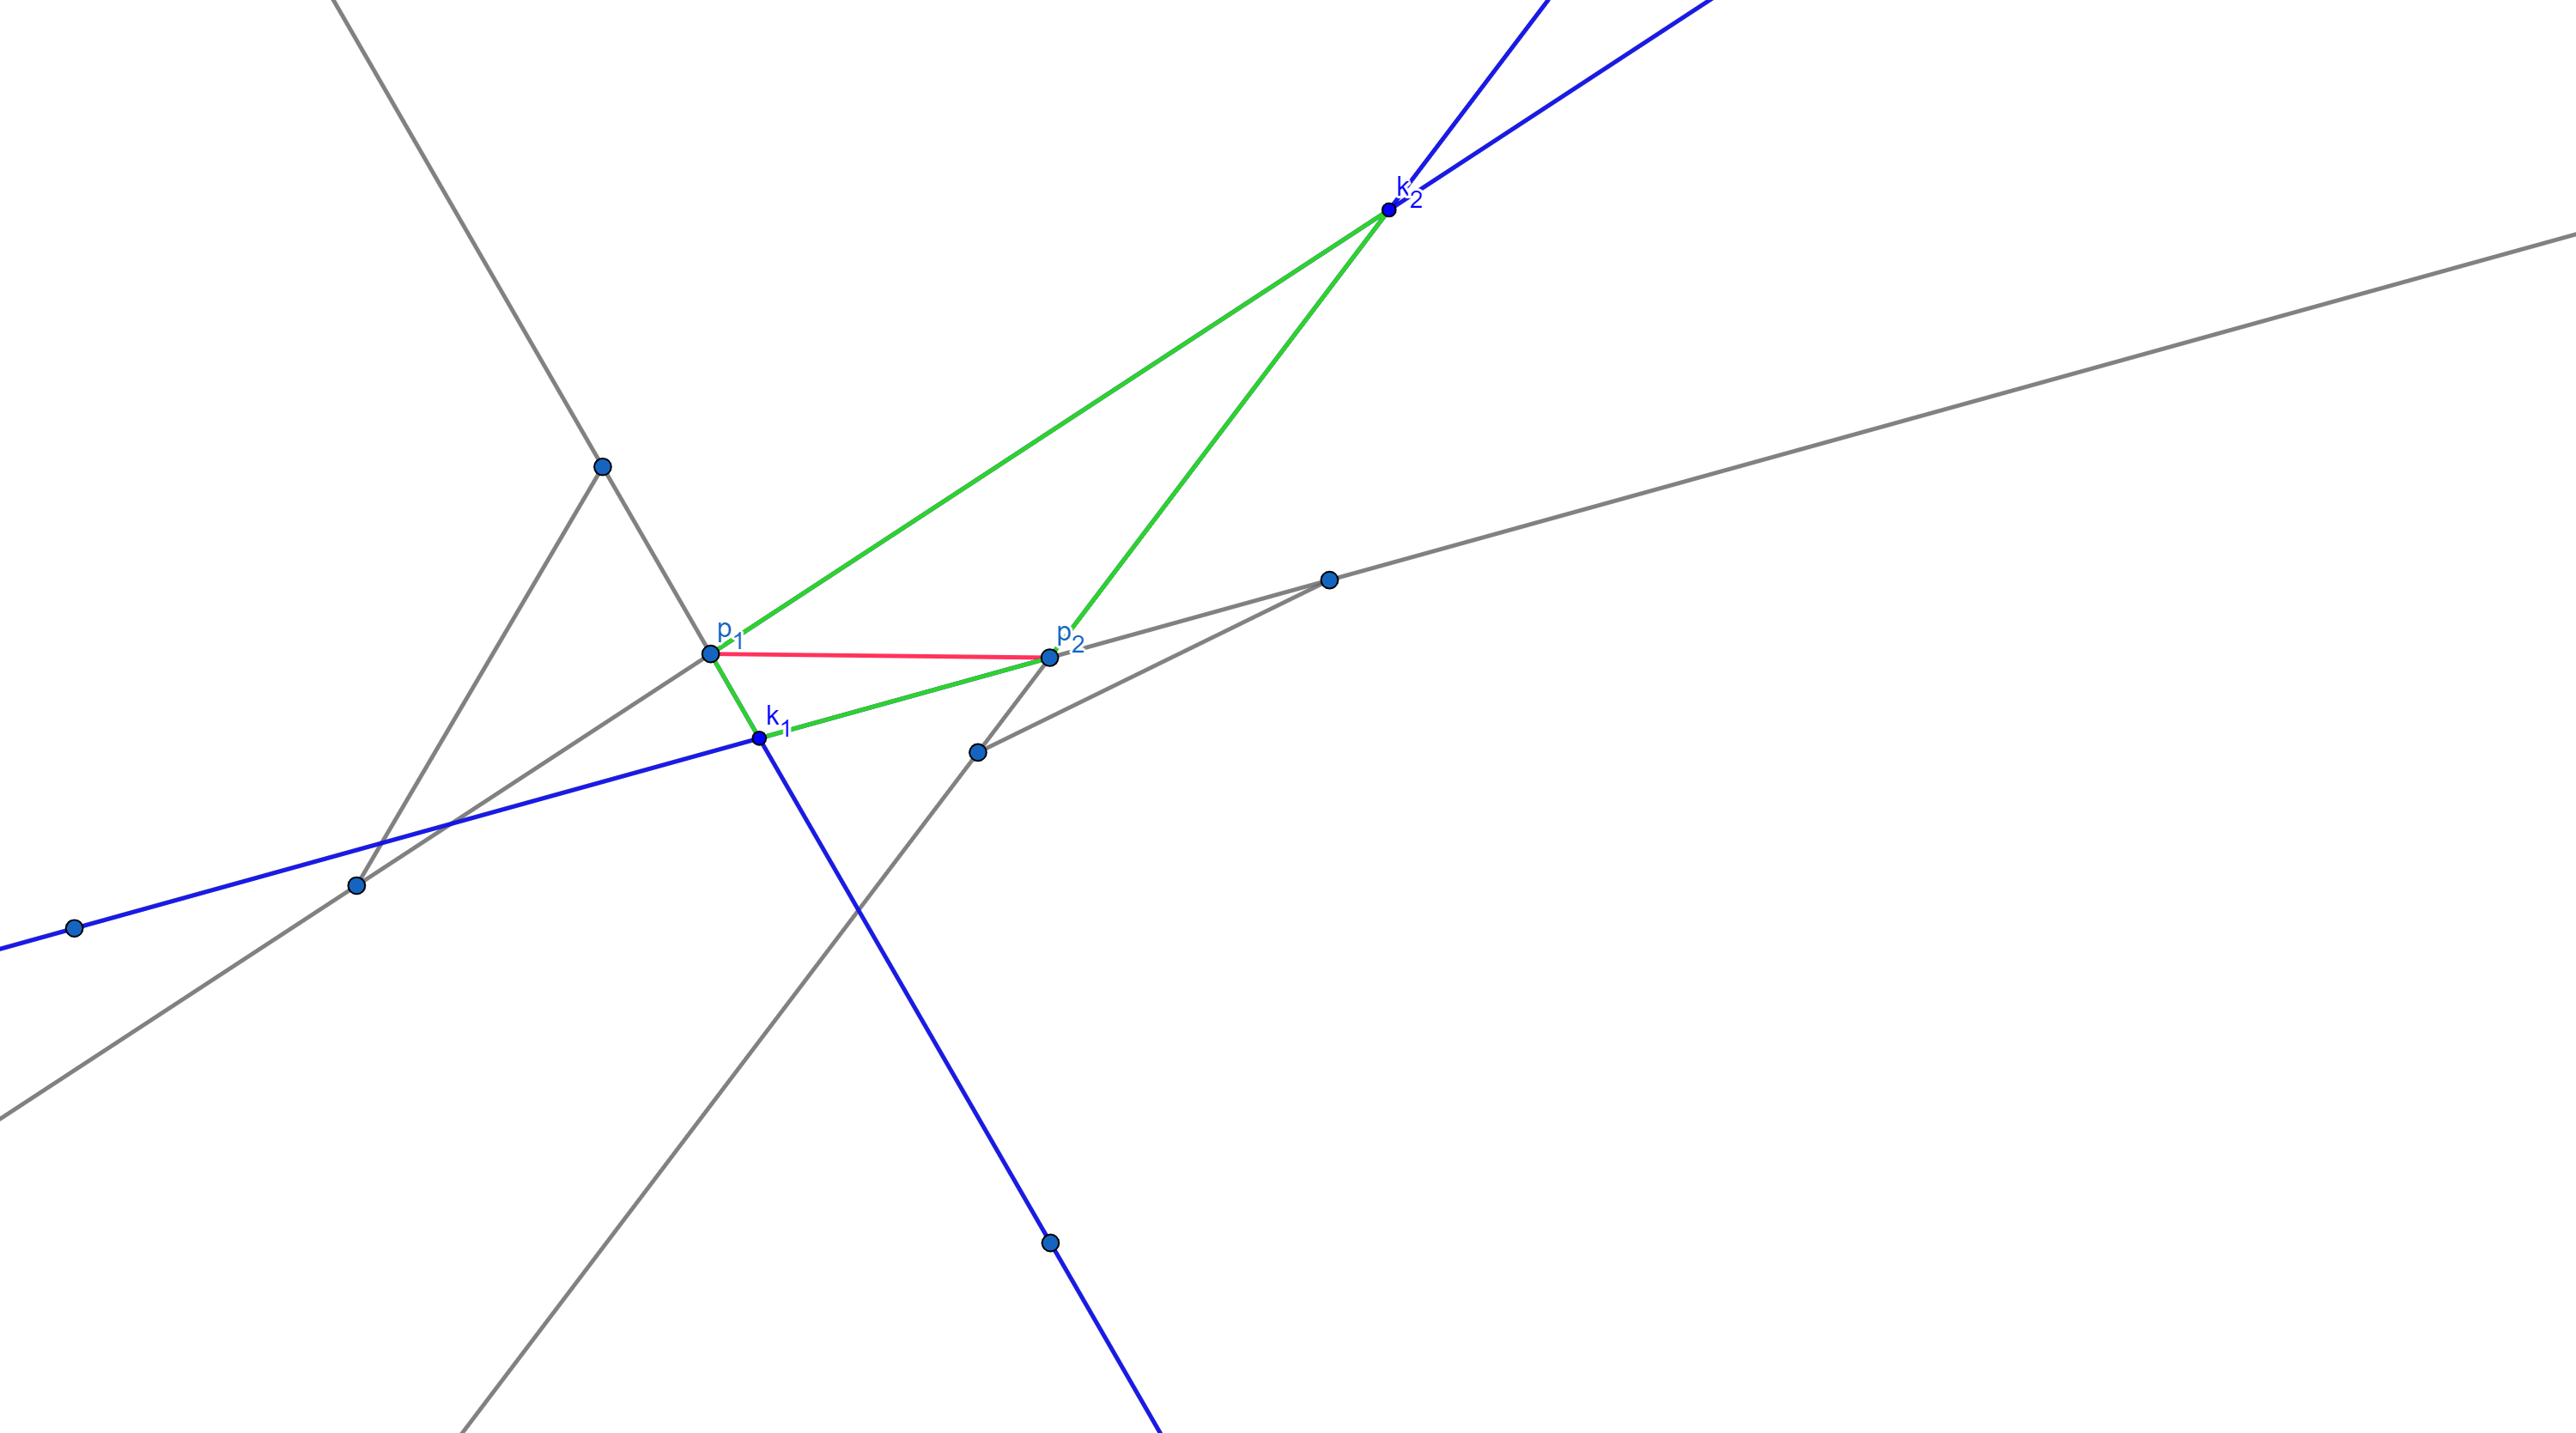
\includegraphics[width=0.5\linewidth]{nozone_2_3.png}
            \end{figure}
      \item Оставшиеся пары ведут себя одинакого, рассмотрим
            $S_1$ и $S_3$. Обе порождаемые зоны имеют луч с
            началом в $p_1$ в правой полуплоскости, 
            один всегда будет <<сильнее>> второго и более
            <<слабый>> можно отбросить. Если отброшенным оказался
            луч, порожденный $S_1$, то оставшиеся лучи в правой
            полуплоскости могут пересечься в точке $k_1$
            и вырезать конструкцией луч-$k_1$-луч кусок из
            итогового множества. Итого результат: множество, 
            ограниченное либо конструкциями луч-$p_1$-луч, 
            луч-$k_1$-луч, либо только луч-$p_1$-луч.
            \begin{figure}[H]
                  \centering
                  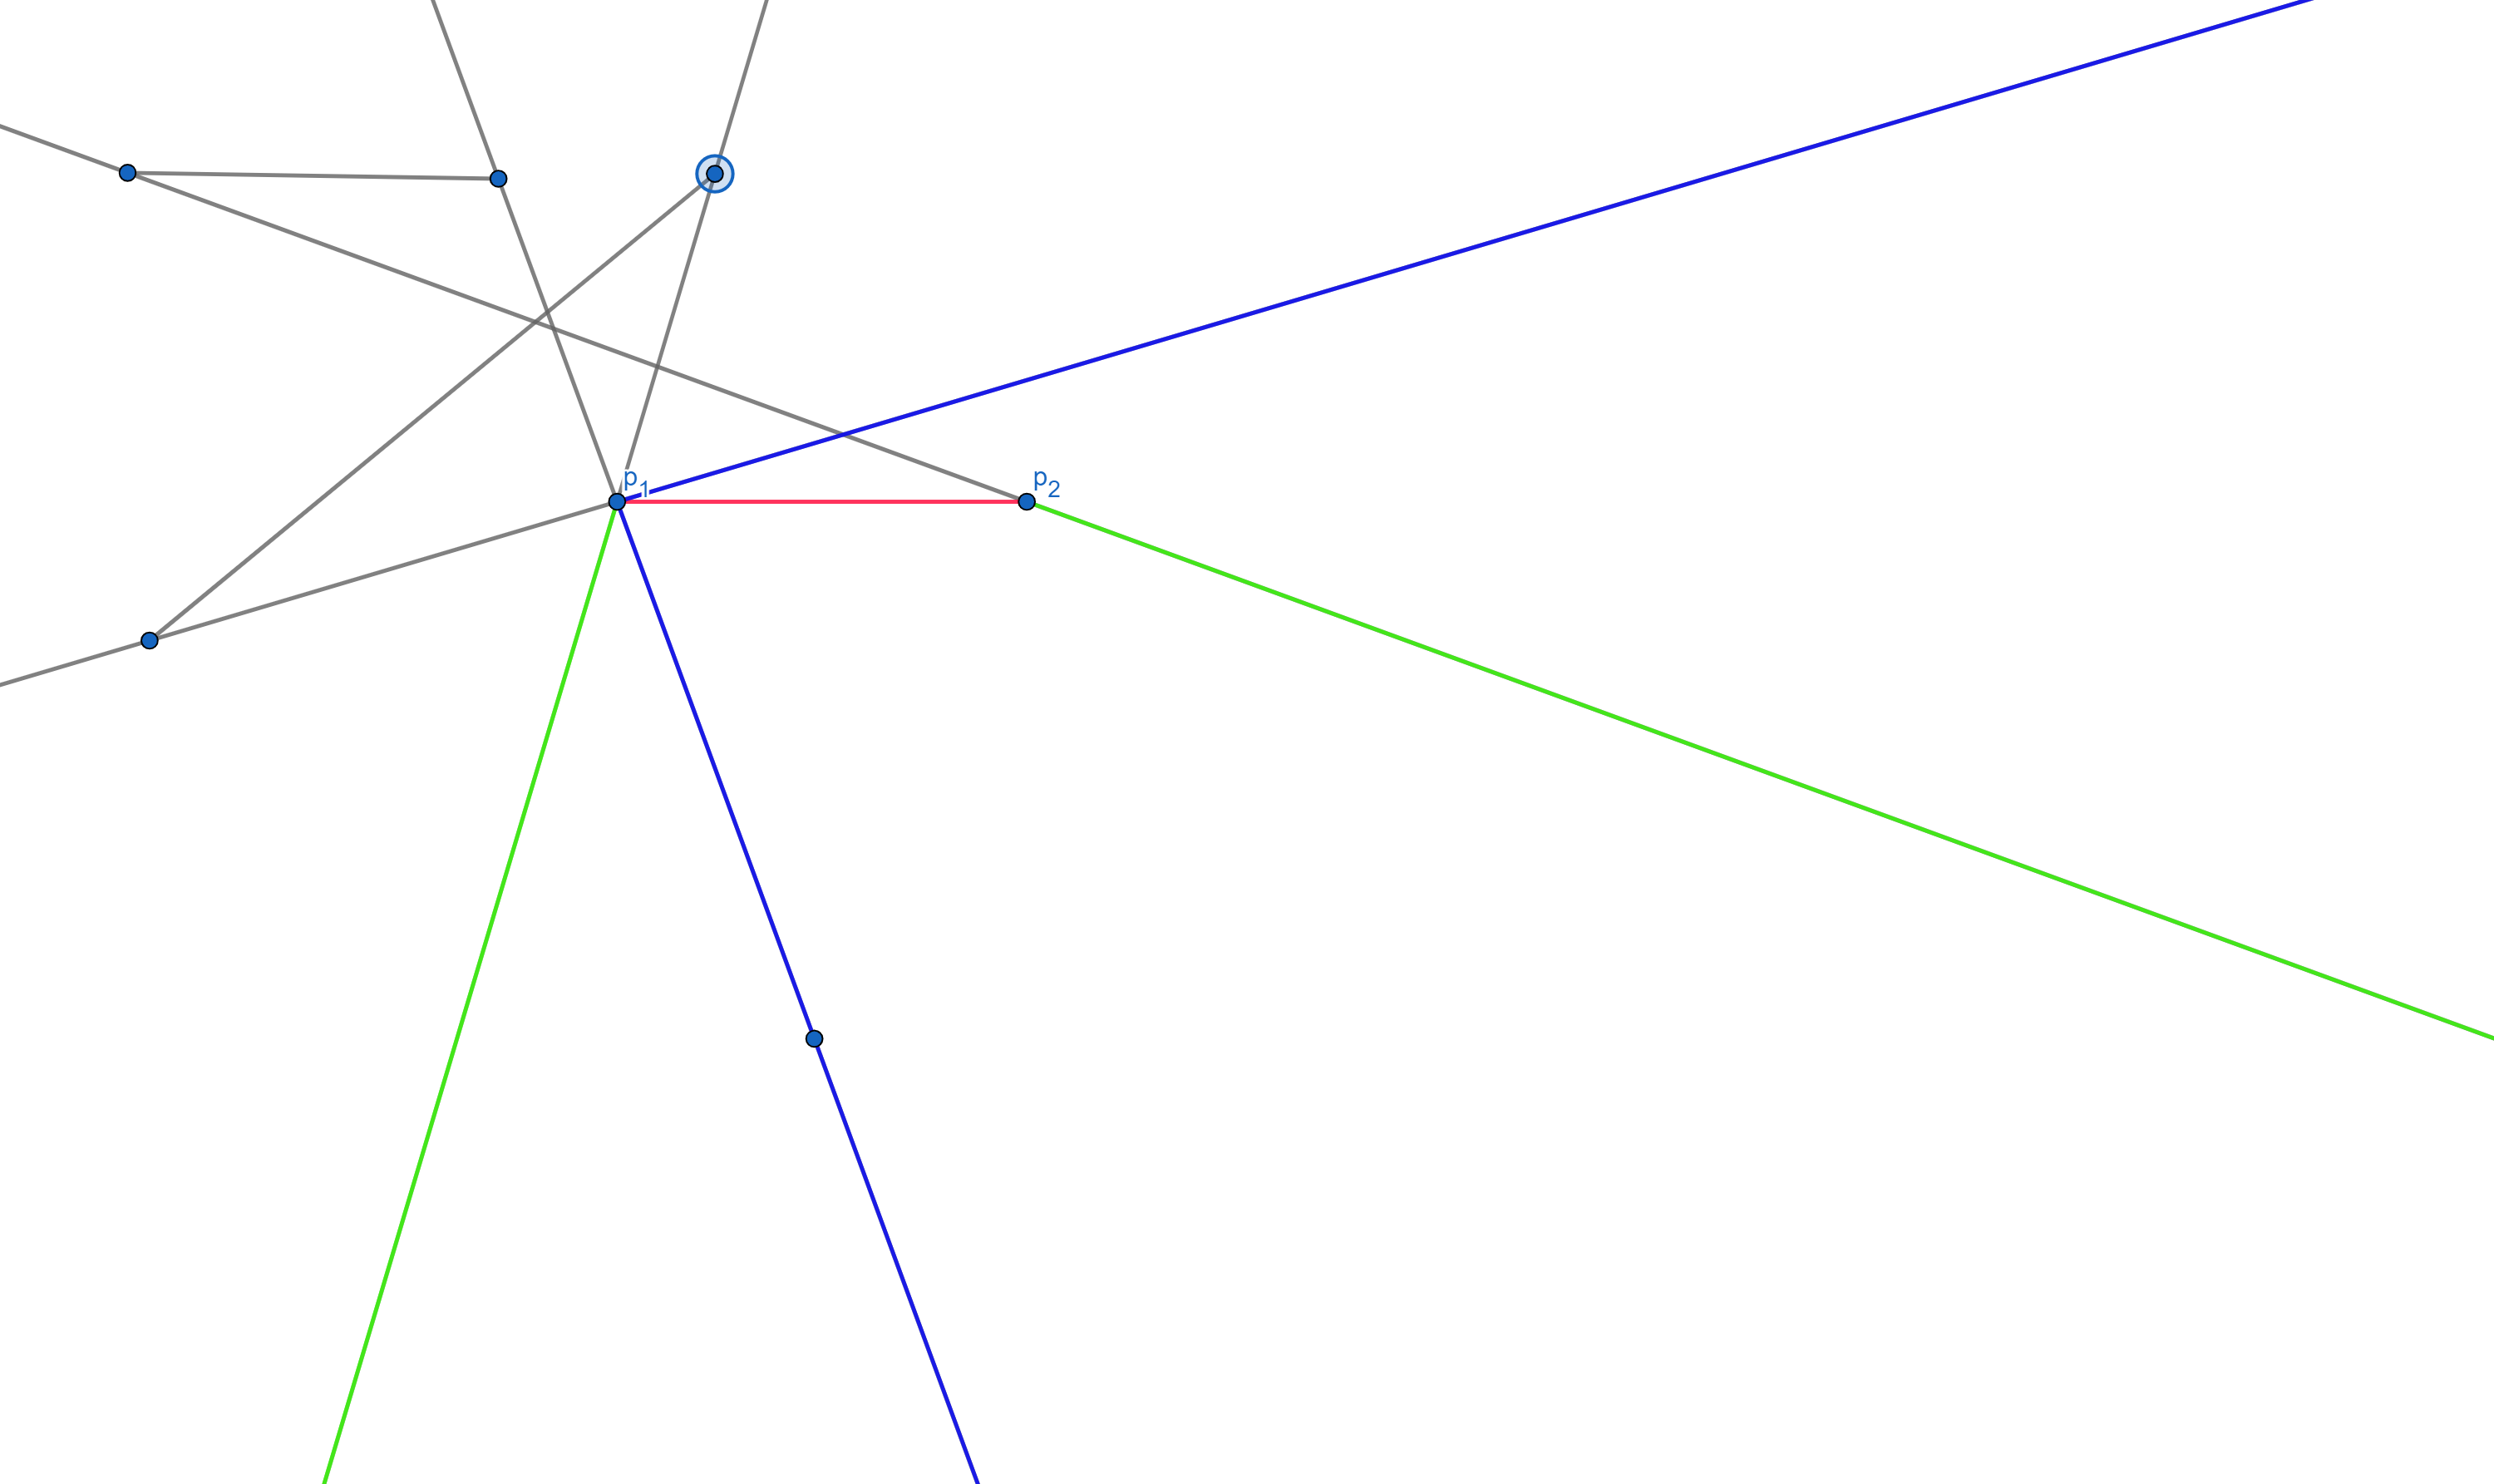
\includegraphics[width=0.5\linewidth]{nozone_2_4.png}
            \end{figure}
            \begin{figure}[H]
                  \centering
                  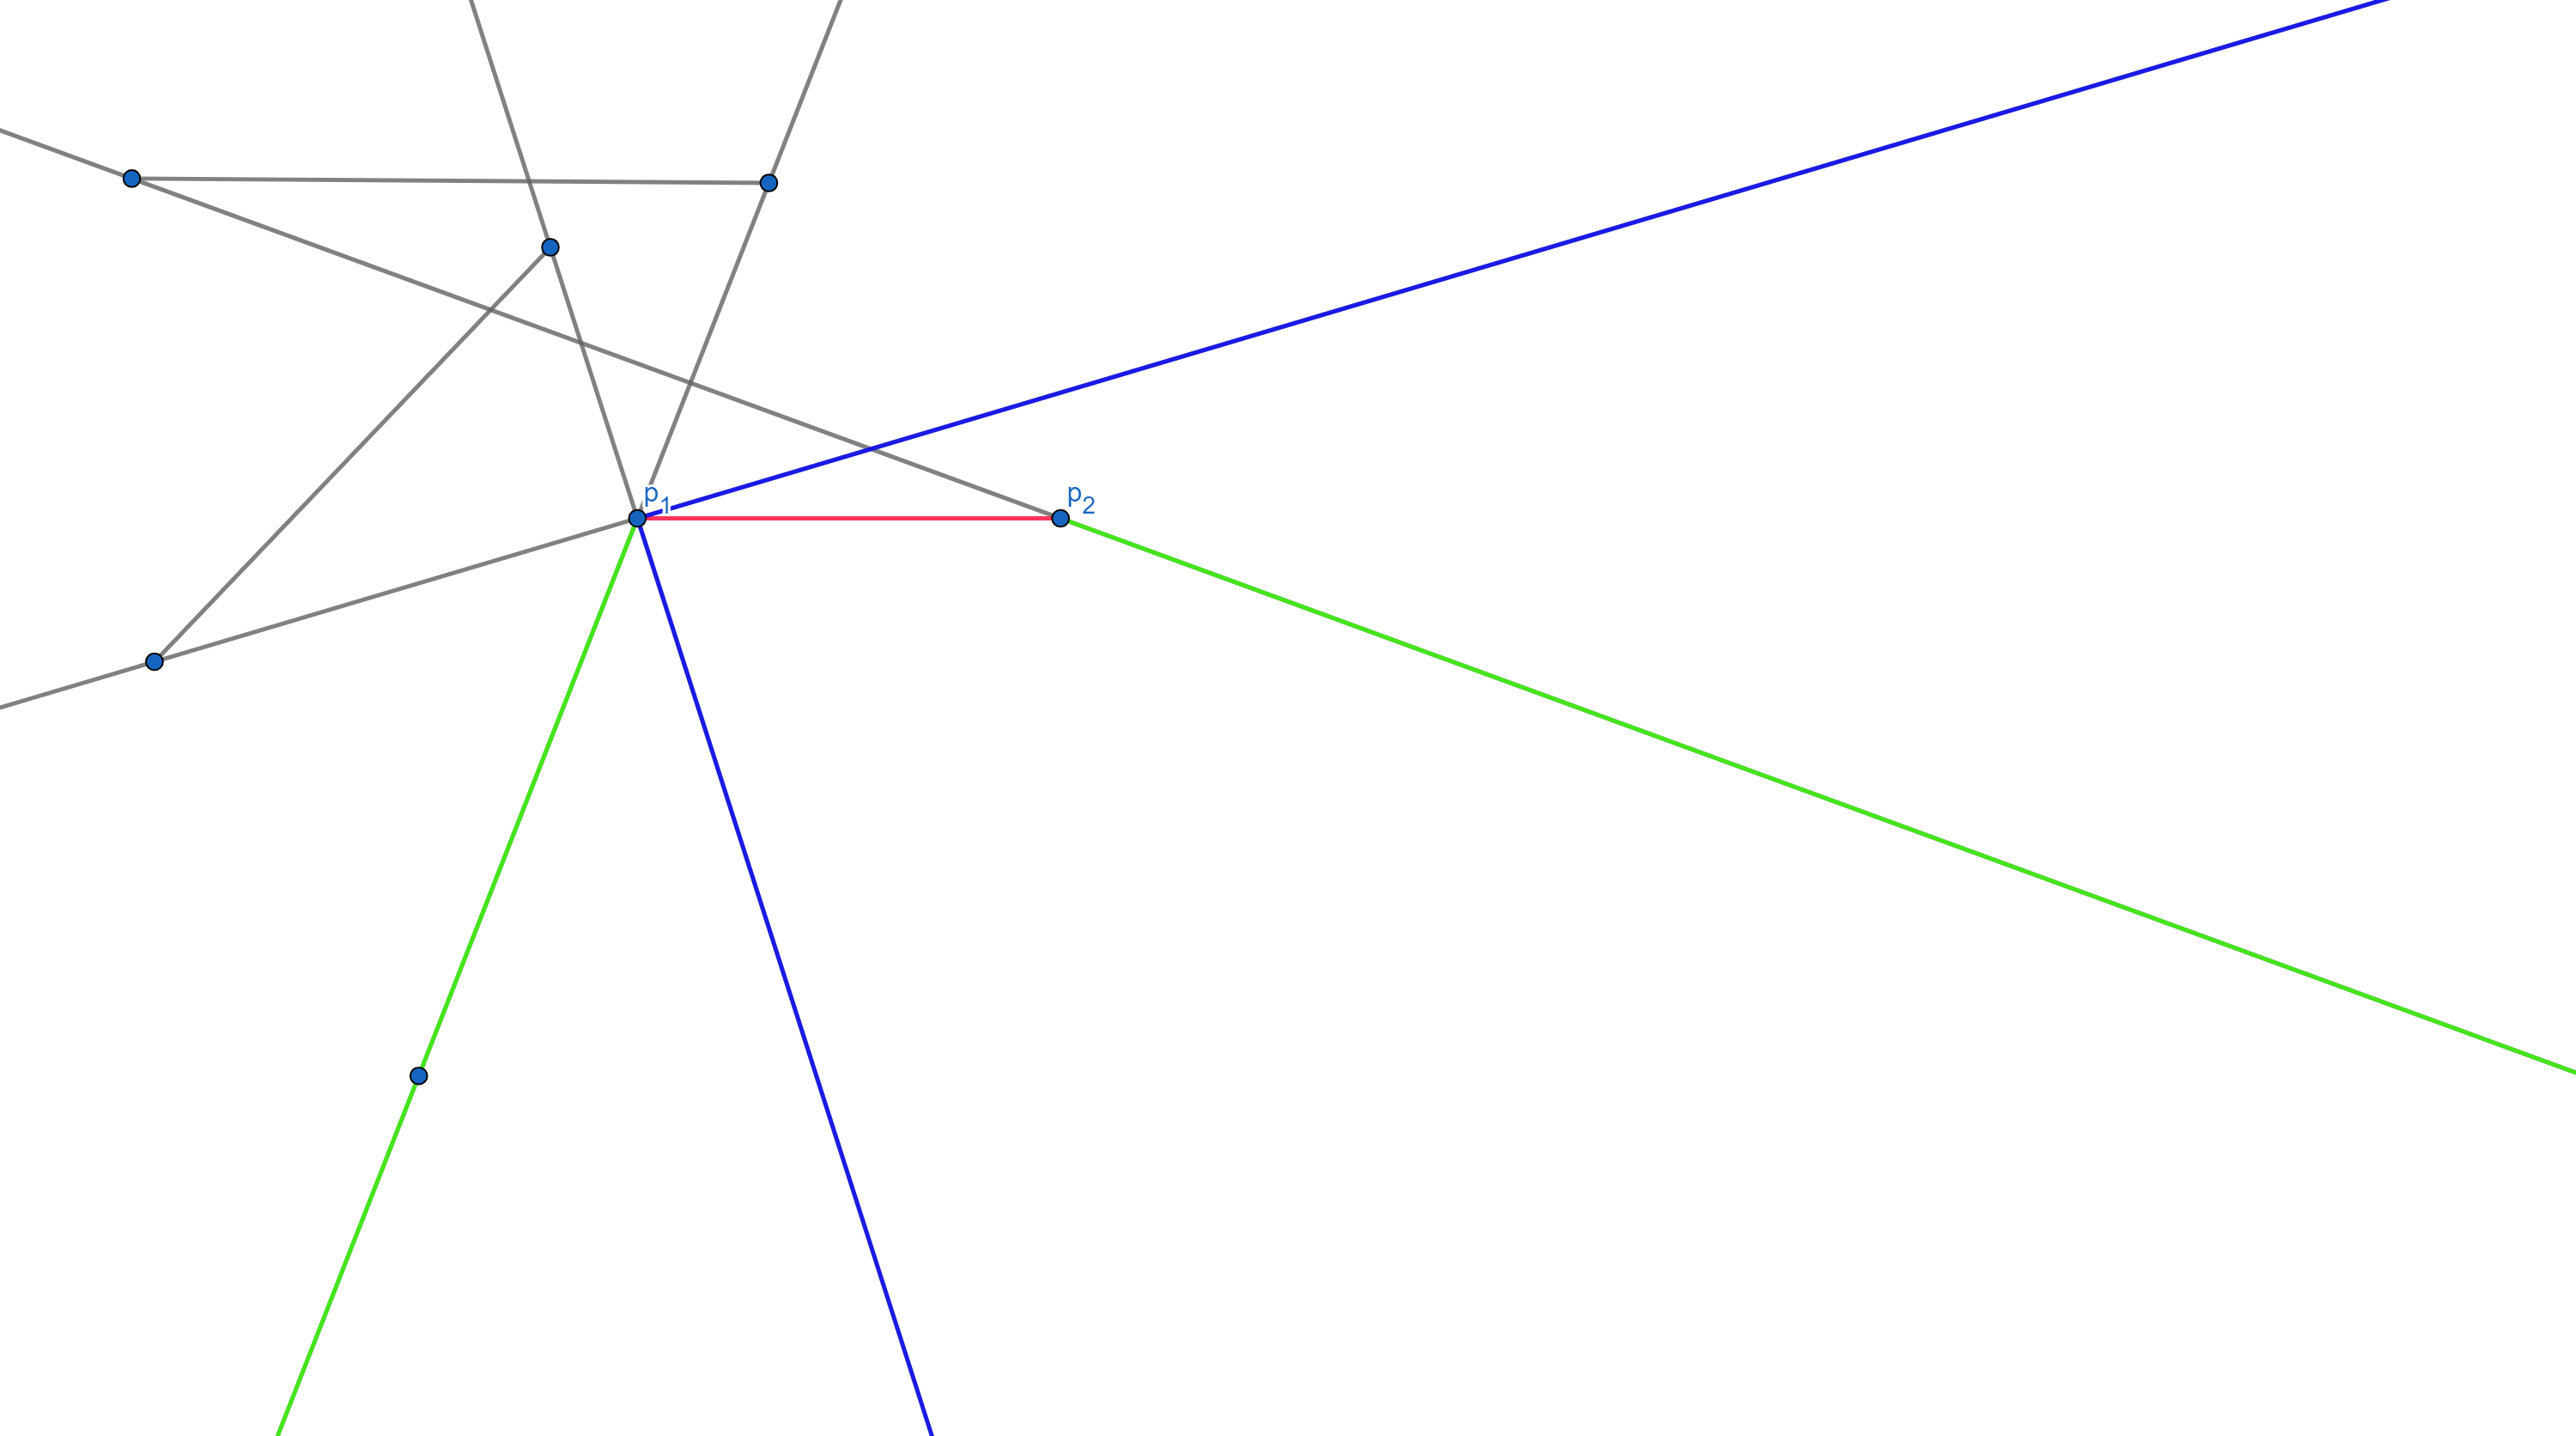
\includegraphics[width=0.5\linewidth]{nozone_2_5.png}
            \end{figure}
            \begin{figure}[H]
                  \centering
                  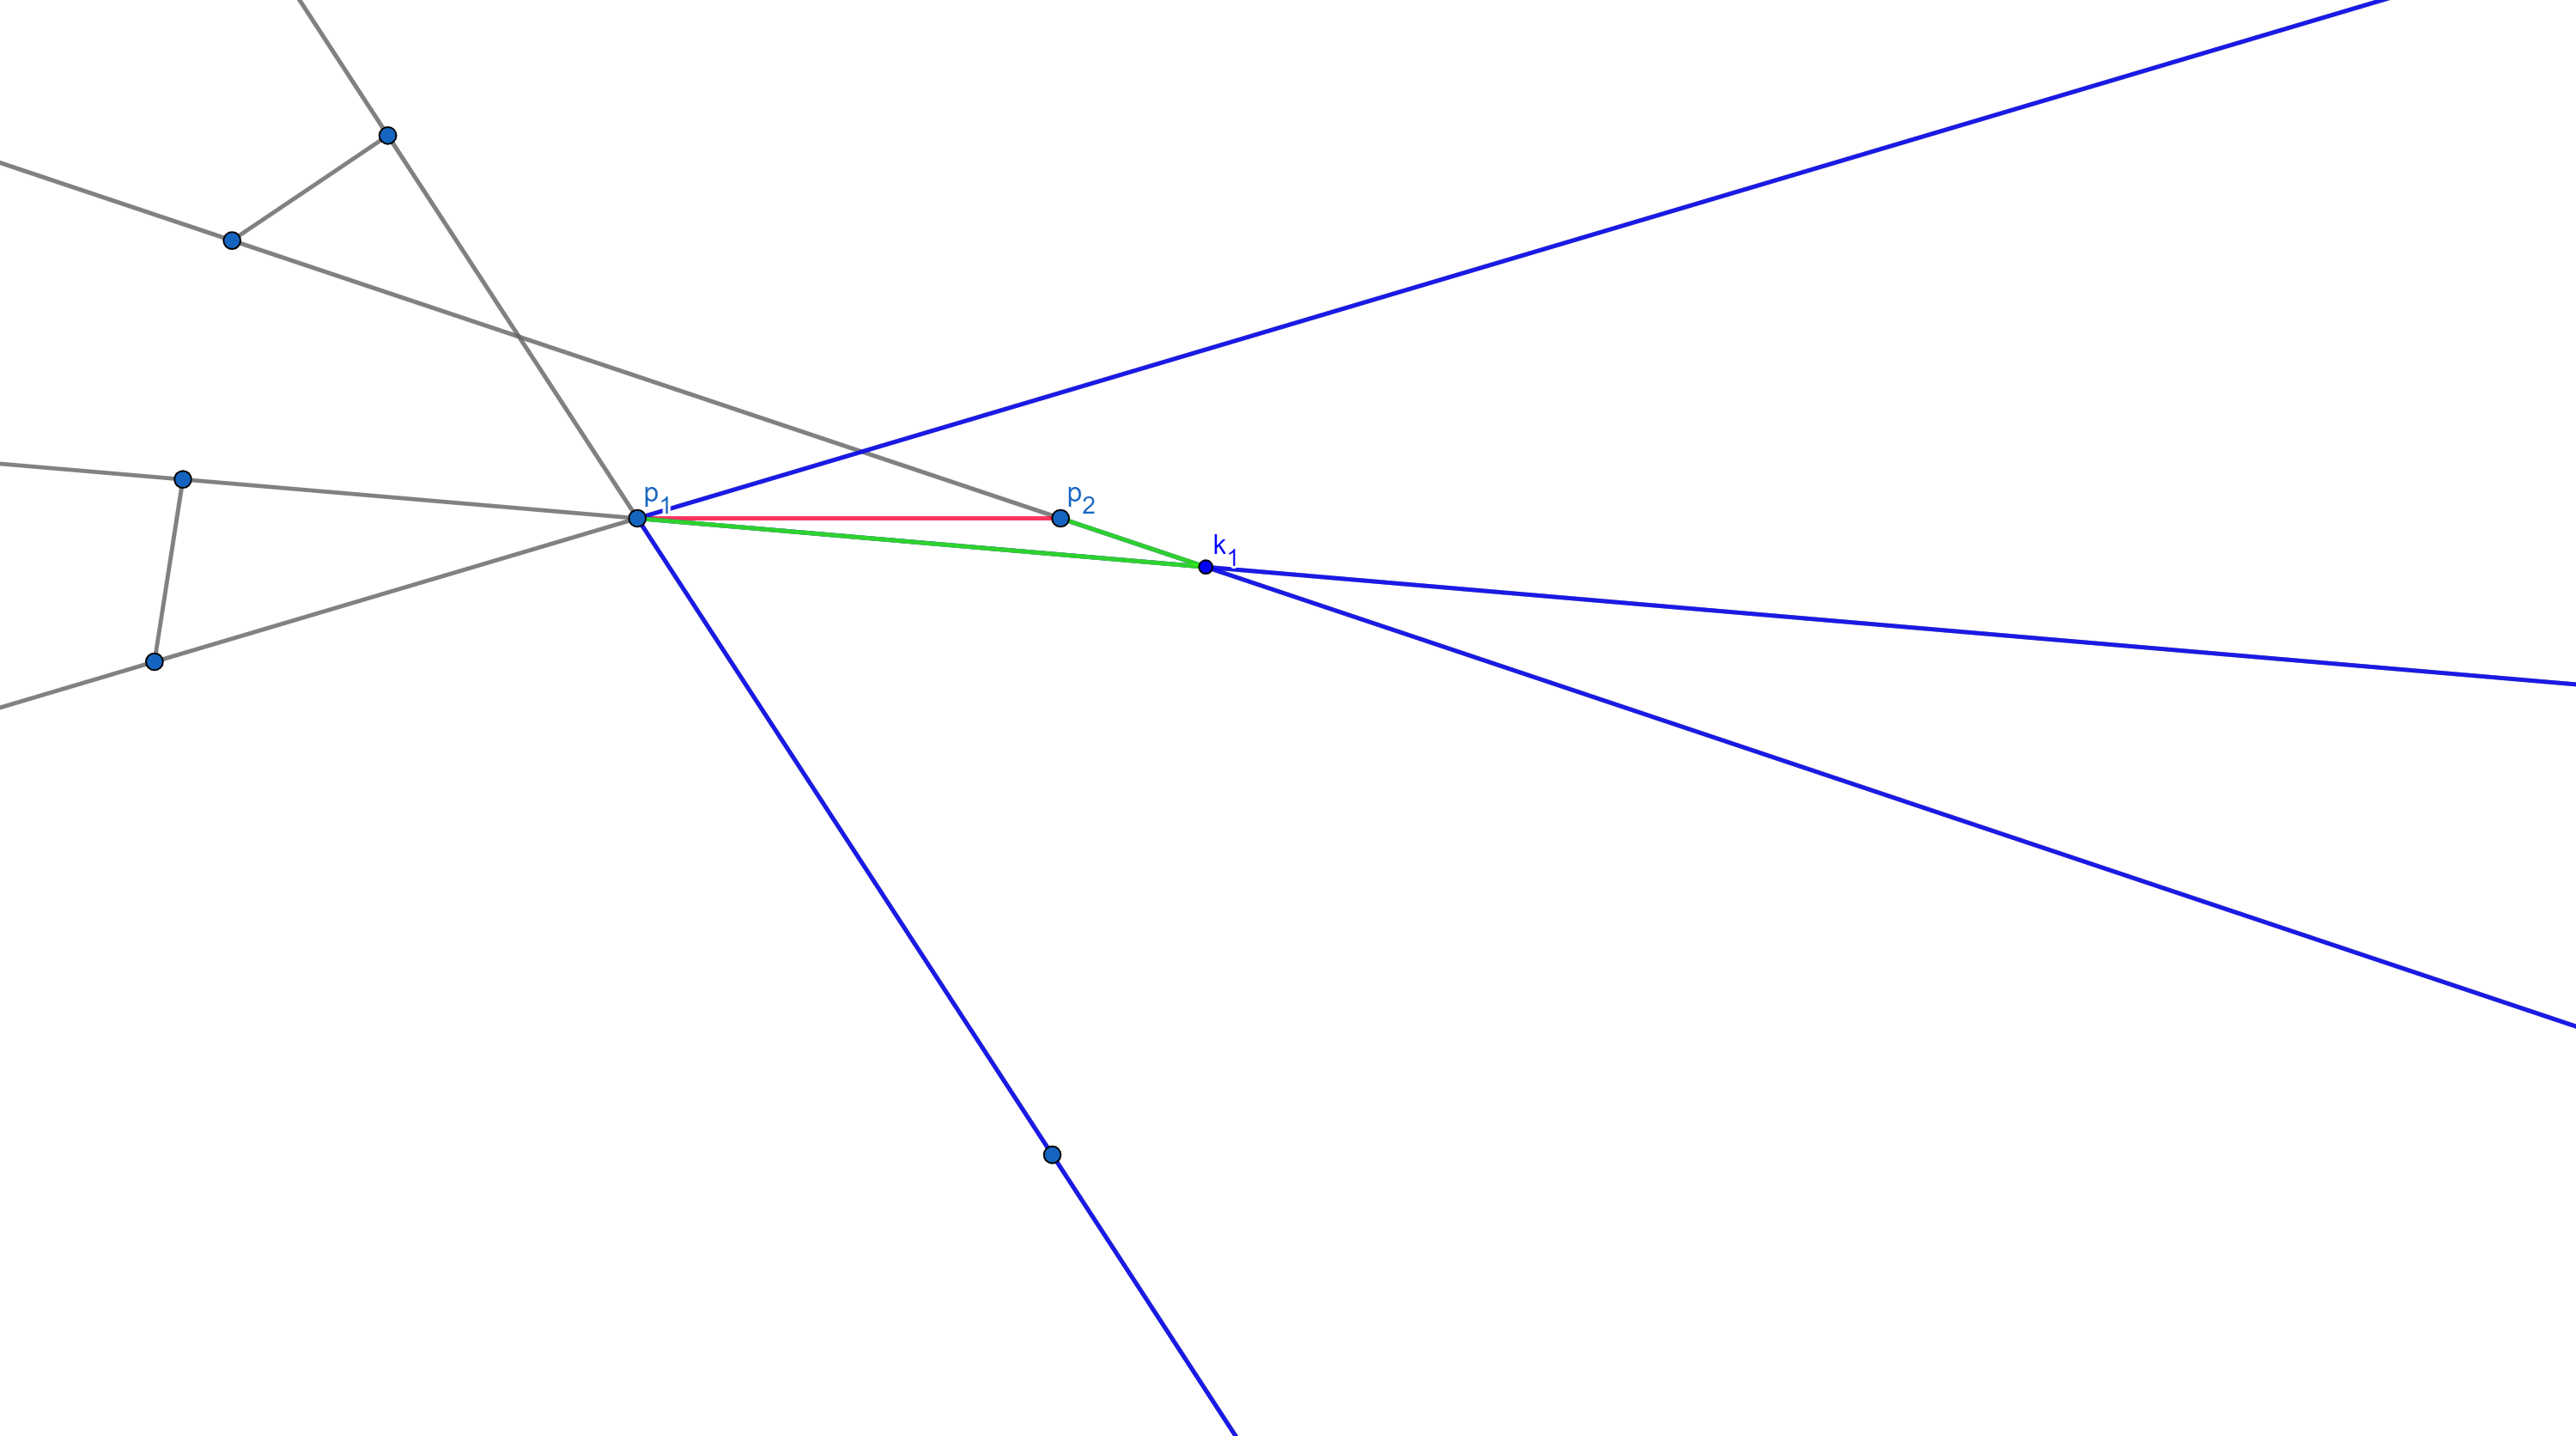
\includegraphics[width=0.5\linewidth]{nozone_2_6.png}
            \end{figure}
      \item Среди троек имеет смысл рассмотреть случай пустого
            $S_2$ (для $S_1$ аналогично) и пустого $S_4$ 
            (для $S_3$ аналогично).
            В случае пустого $S_2$ весь интерес сводится к наличию
            пересечения лучей, порождаемых $S_3$ и $S_4$, в правой 
            полуплоскости. Если пересечения нет, то оно будет в
            левой полуплоскости, а порождаемая им луч-$k_2$-луч будет
            единственным ограничением.
            Если пересечение есть, то конструкция 
            луч-$k_1$-луч может пересечься с лучами, порожденными
            $S_1$ в 1-2 точках. (обозначим их $k_3$, $k_4$).
            Если пересечения нет, то и ограничений в нижней половине
            нет. Иначе ограничения - контрукции луч-$k_3$-луч,
            луч-$k_4$-луч. Итого результат: множество, 
            ограниченное в левой полуплоскости либо
            луч-$k_2$-луч, либо нечем. В правой: либо луч-$k_3$-луч,
            либо луч-$k_4$-луч, либо луч-$k_3$-луч, луч-$k_4$-луч, 
            либо нечем. (8 вариантов, приведем самые интересные)
            \begin{figure}[H]
                  \centering
                  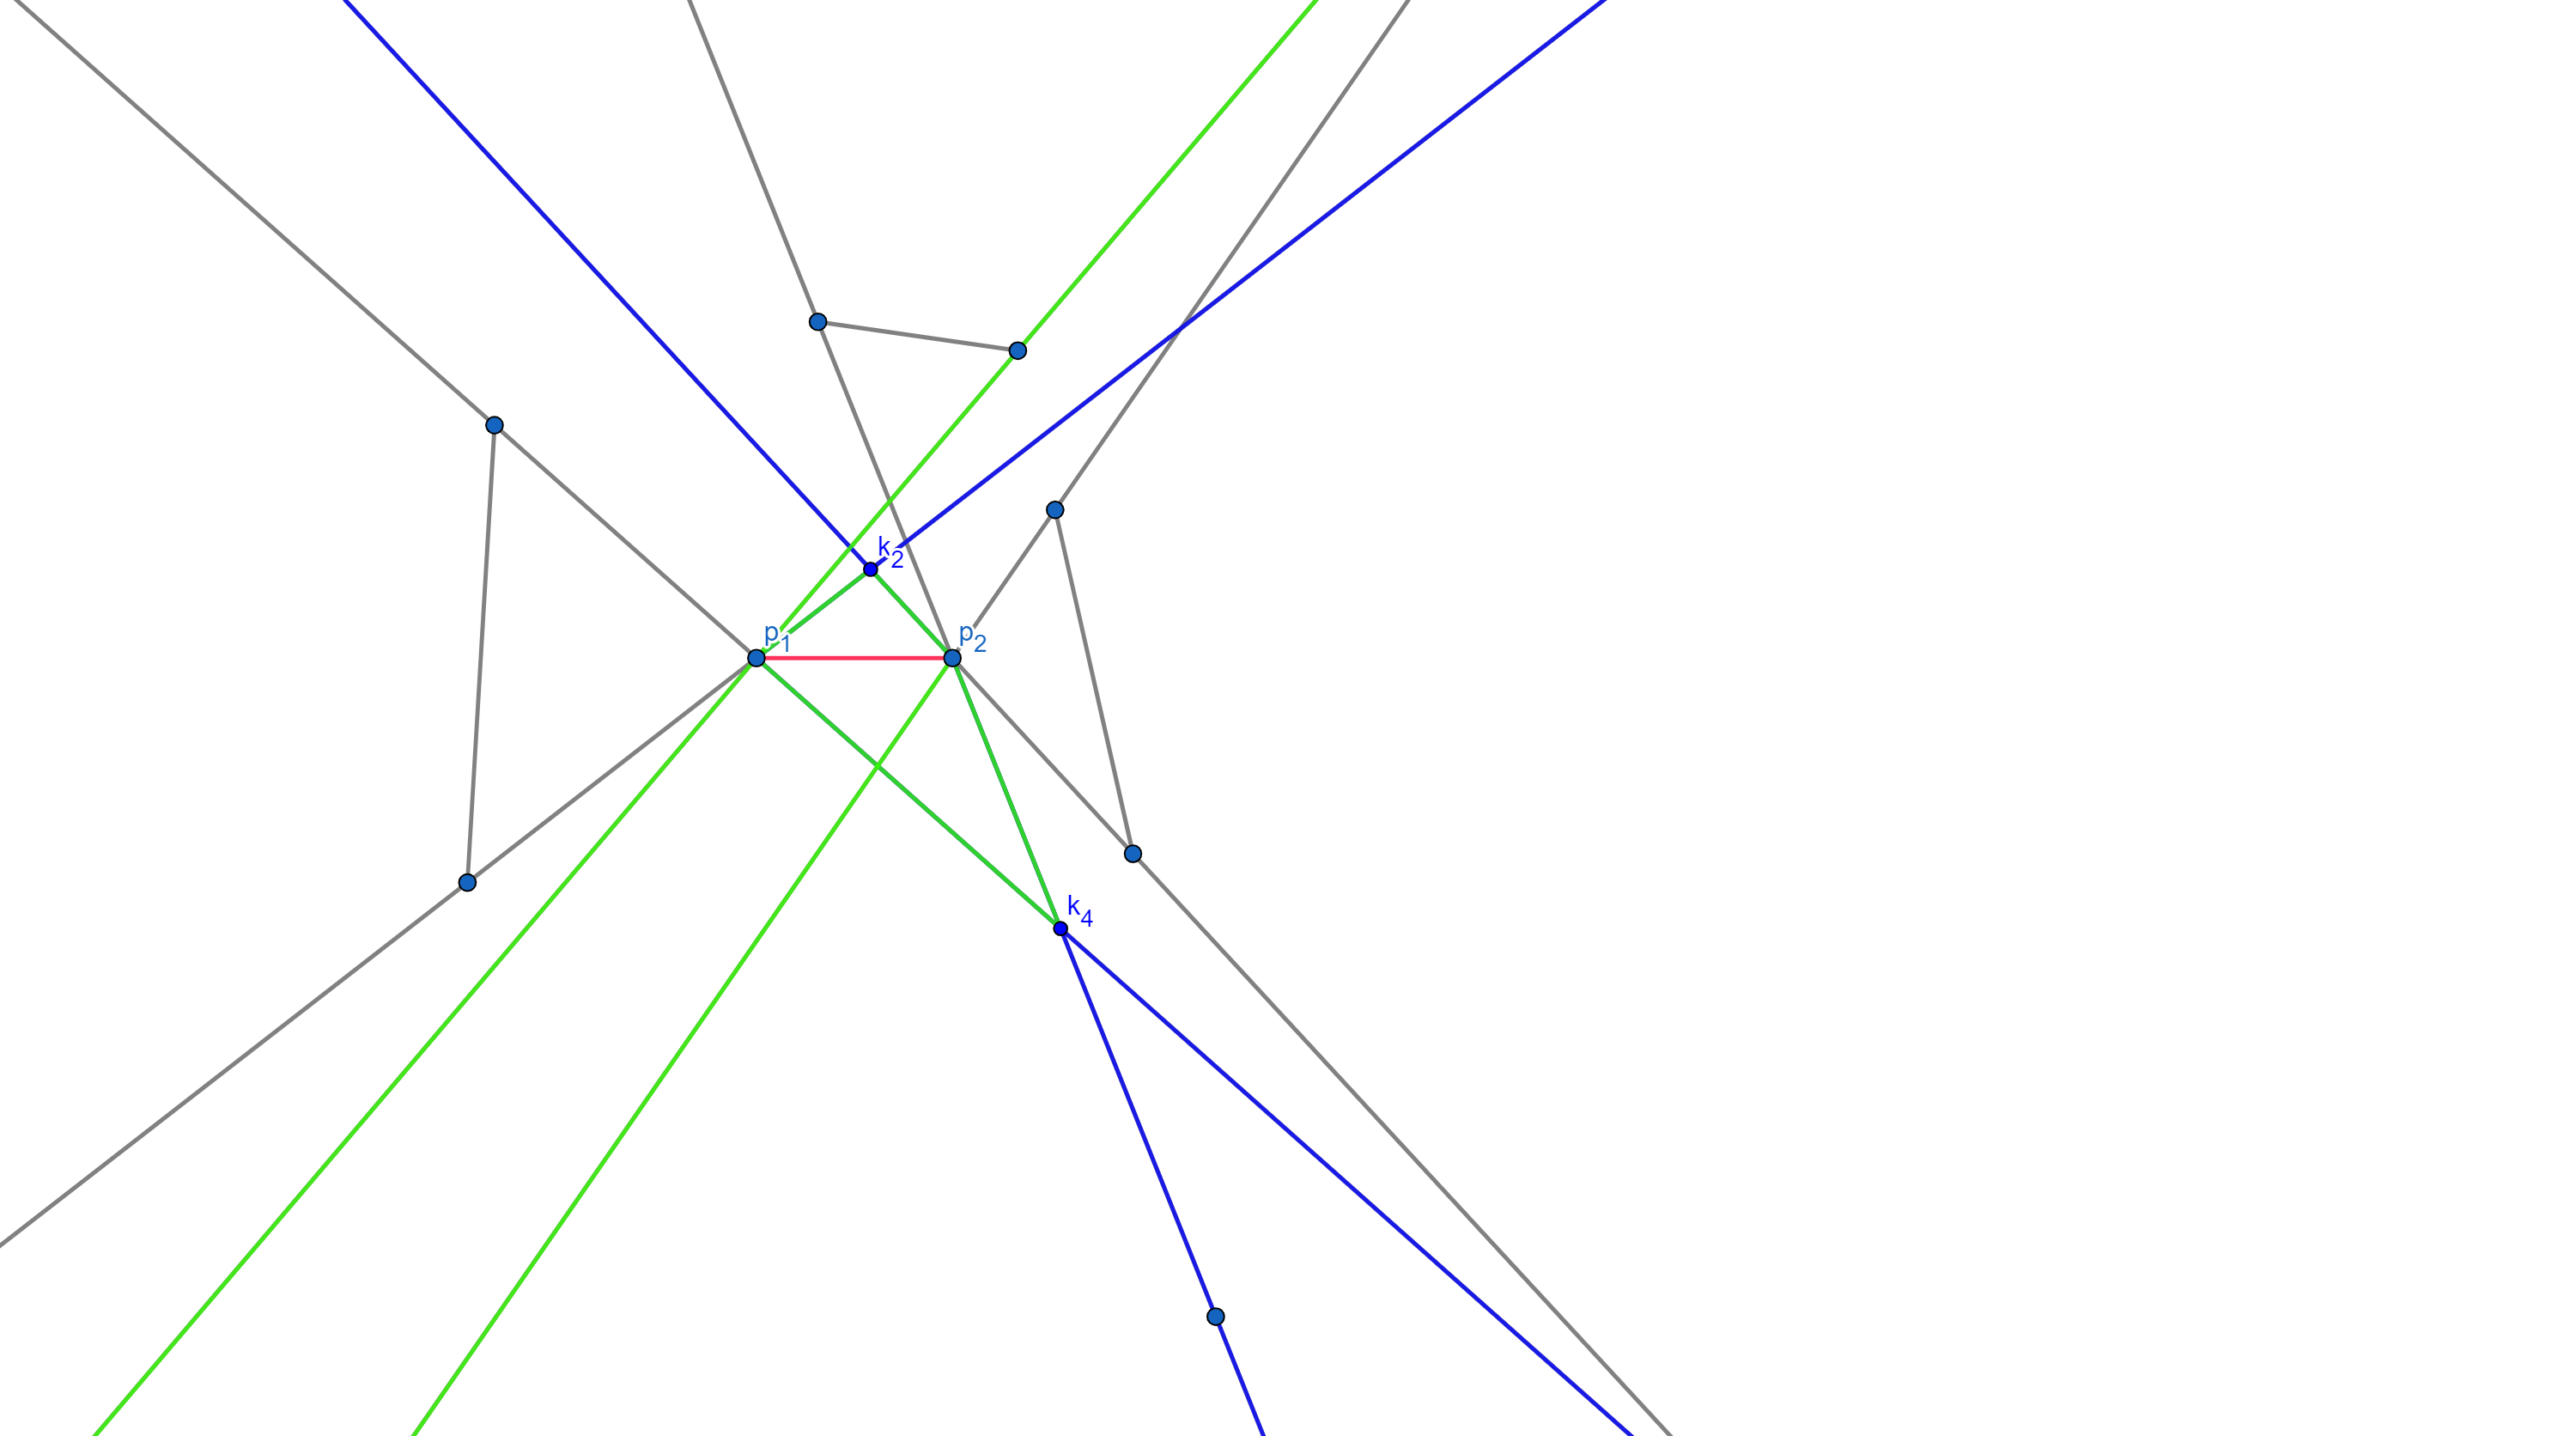
\includegraphics[width=0.5\linewidth]{nozone_3_1.png}
            \end{figure}
            \begin{figure}[H]
                  \centering
                  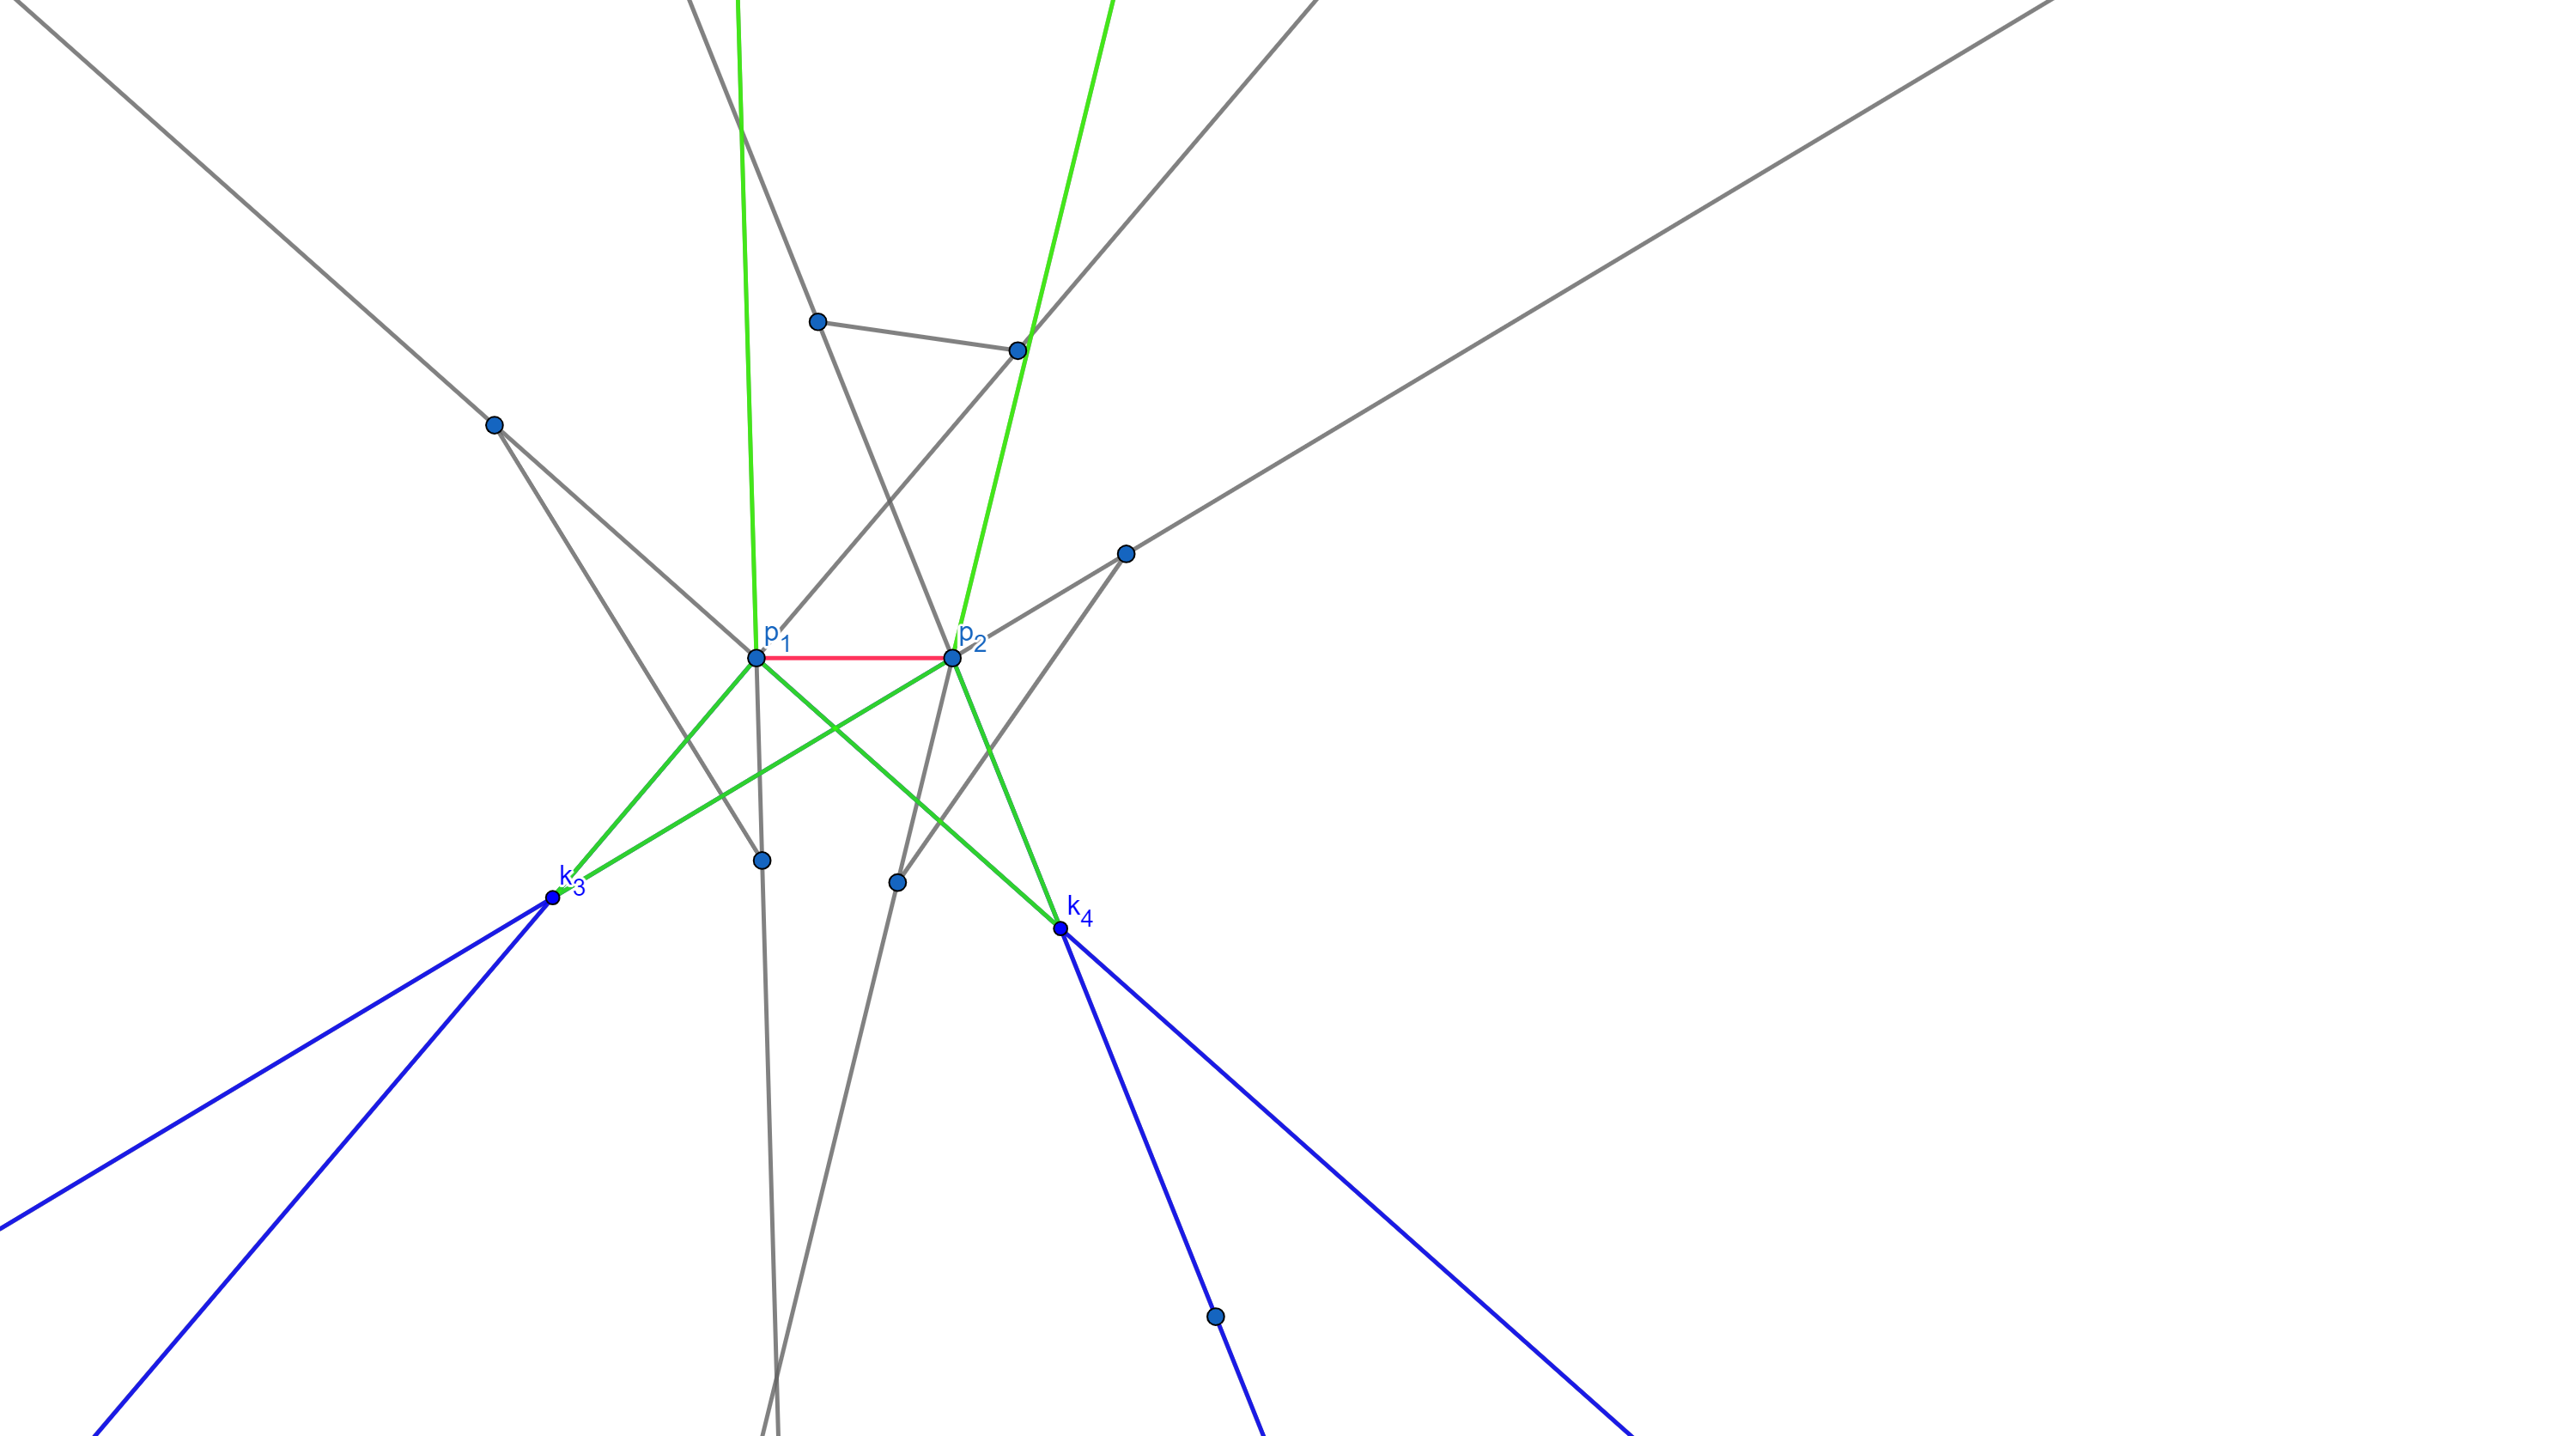
\includegraphics[width=0.5\linewidth]{nozone_3_2.png}
            \end{figure}
      \item В случае пустого $S_4$ весь интерес сводится к наличию
            пересечения лучей $S_3$ и лучами $S_1$, $S_2$ из $p_2$.
            Если пересечение есть (в точках $k_1$, $k_2$), 
            появляются дополнительные ограничения 
            (может быть только одно). Если пересечения нет, то
            зона порождаемая $S_3$ имеет более сильное
            воздействие, чем 2-4 луча, задающие зоны $S_1$, $S_2$.
            Итого результат: множество, ограниченное контрукцией
            луч-$p_1$-луч и либо луч-$k_1$-луч, либо луч-$k_2$-луч, 
            либо луч-$k_1$-луч, луч-$k_2$-луч, либо нечем.
            (4 варианта, приведем самые интересные)
            \begin{figure}[H]
                  \centering
                  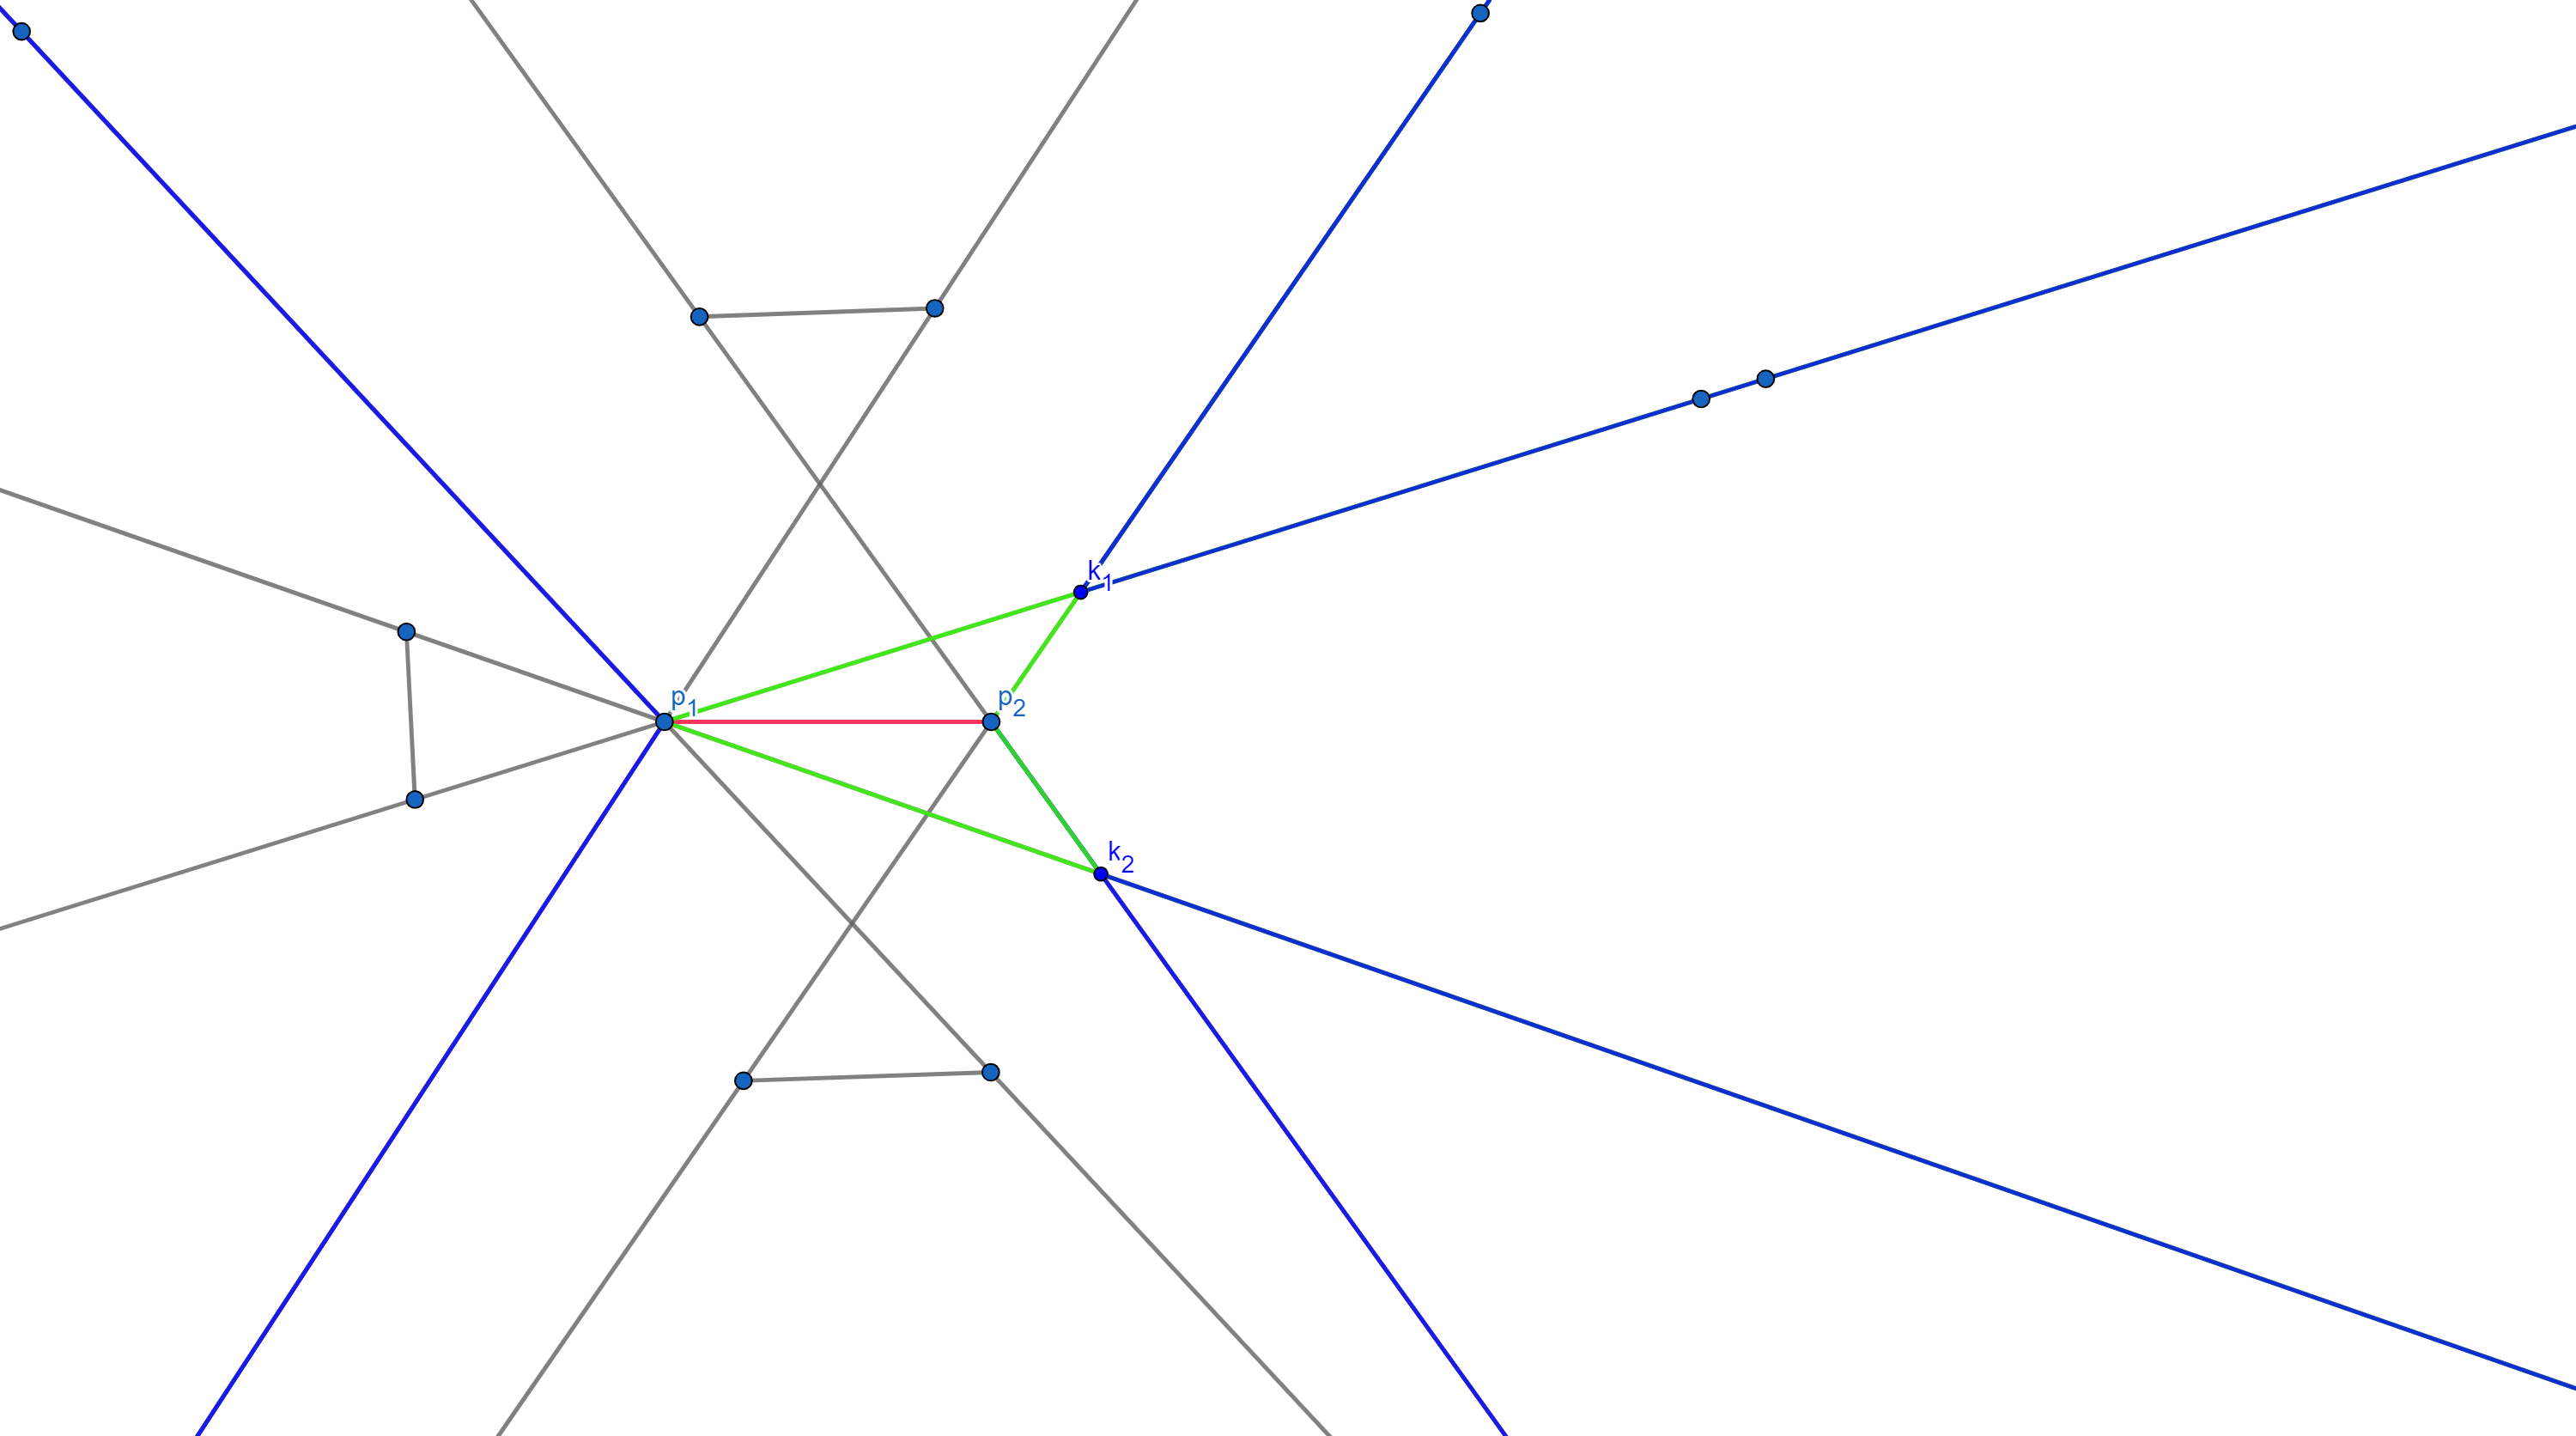
\includegraphics[width=0.5\linewidth]{nozone_3_3.png}
            \end{figure}
            \begin{figure}[H]
                  \centering
                  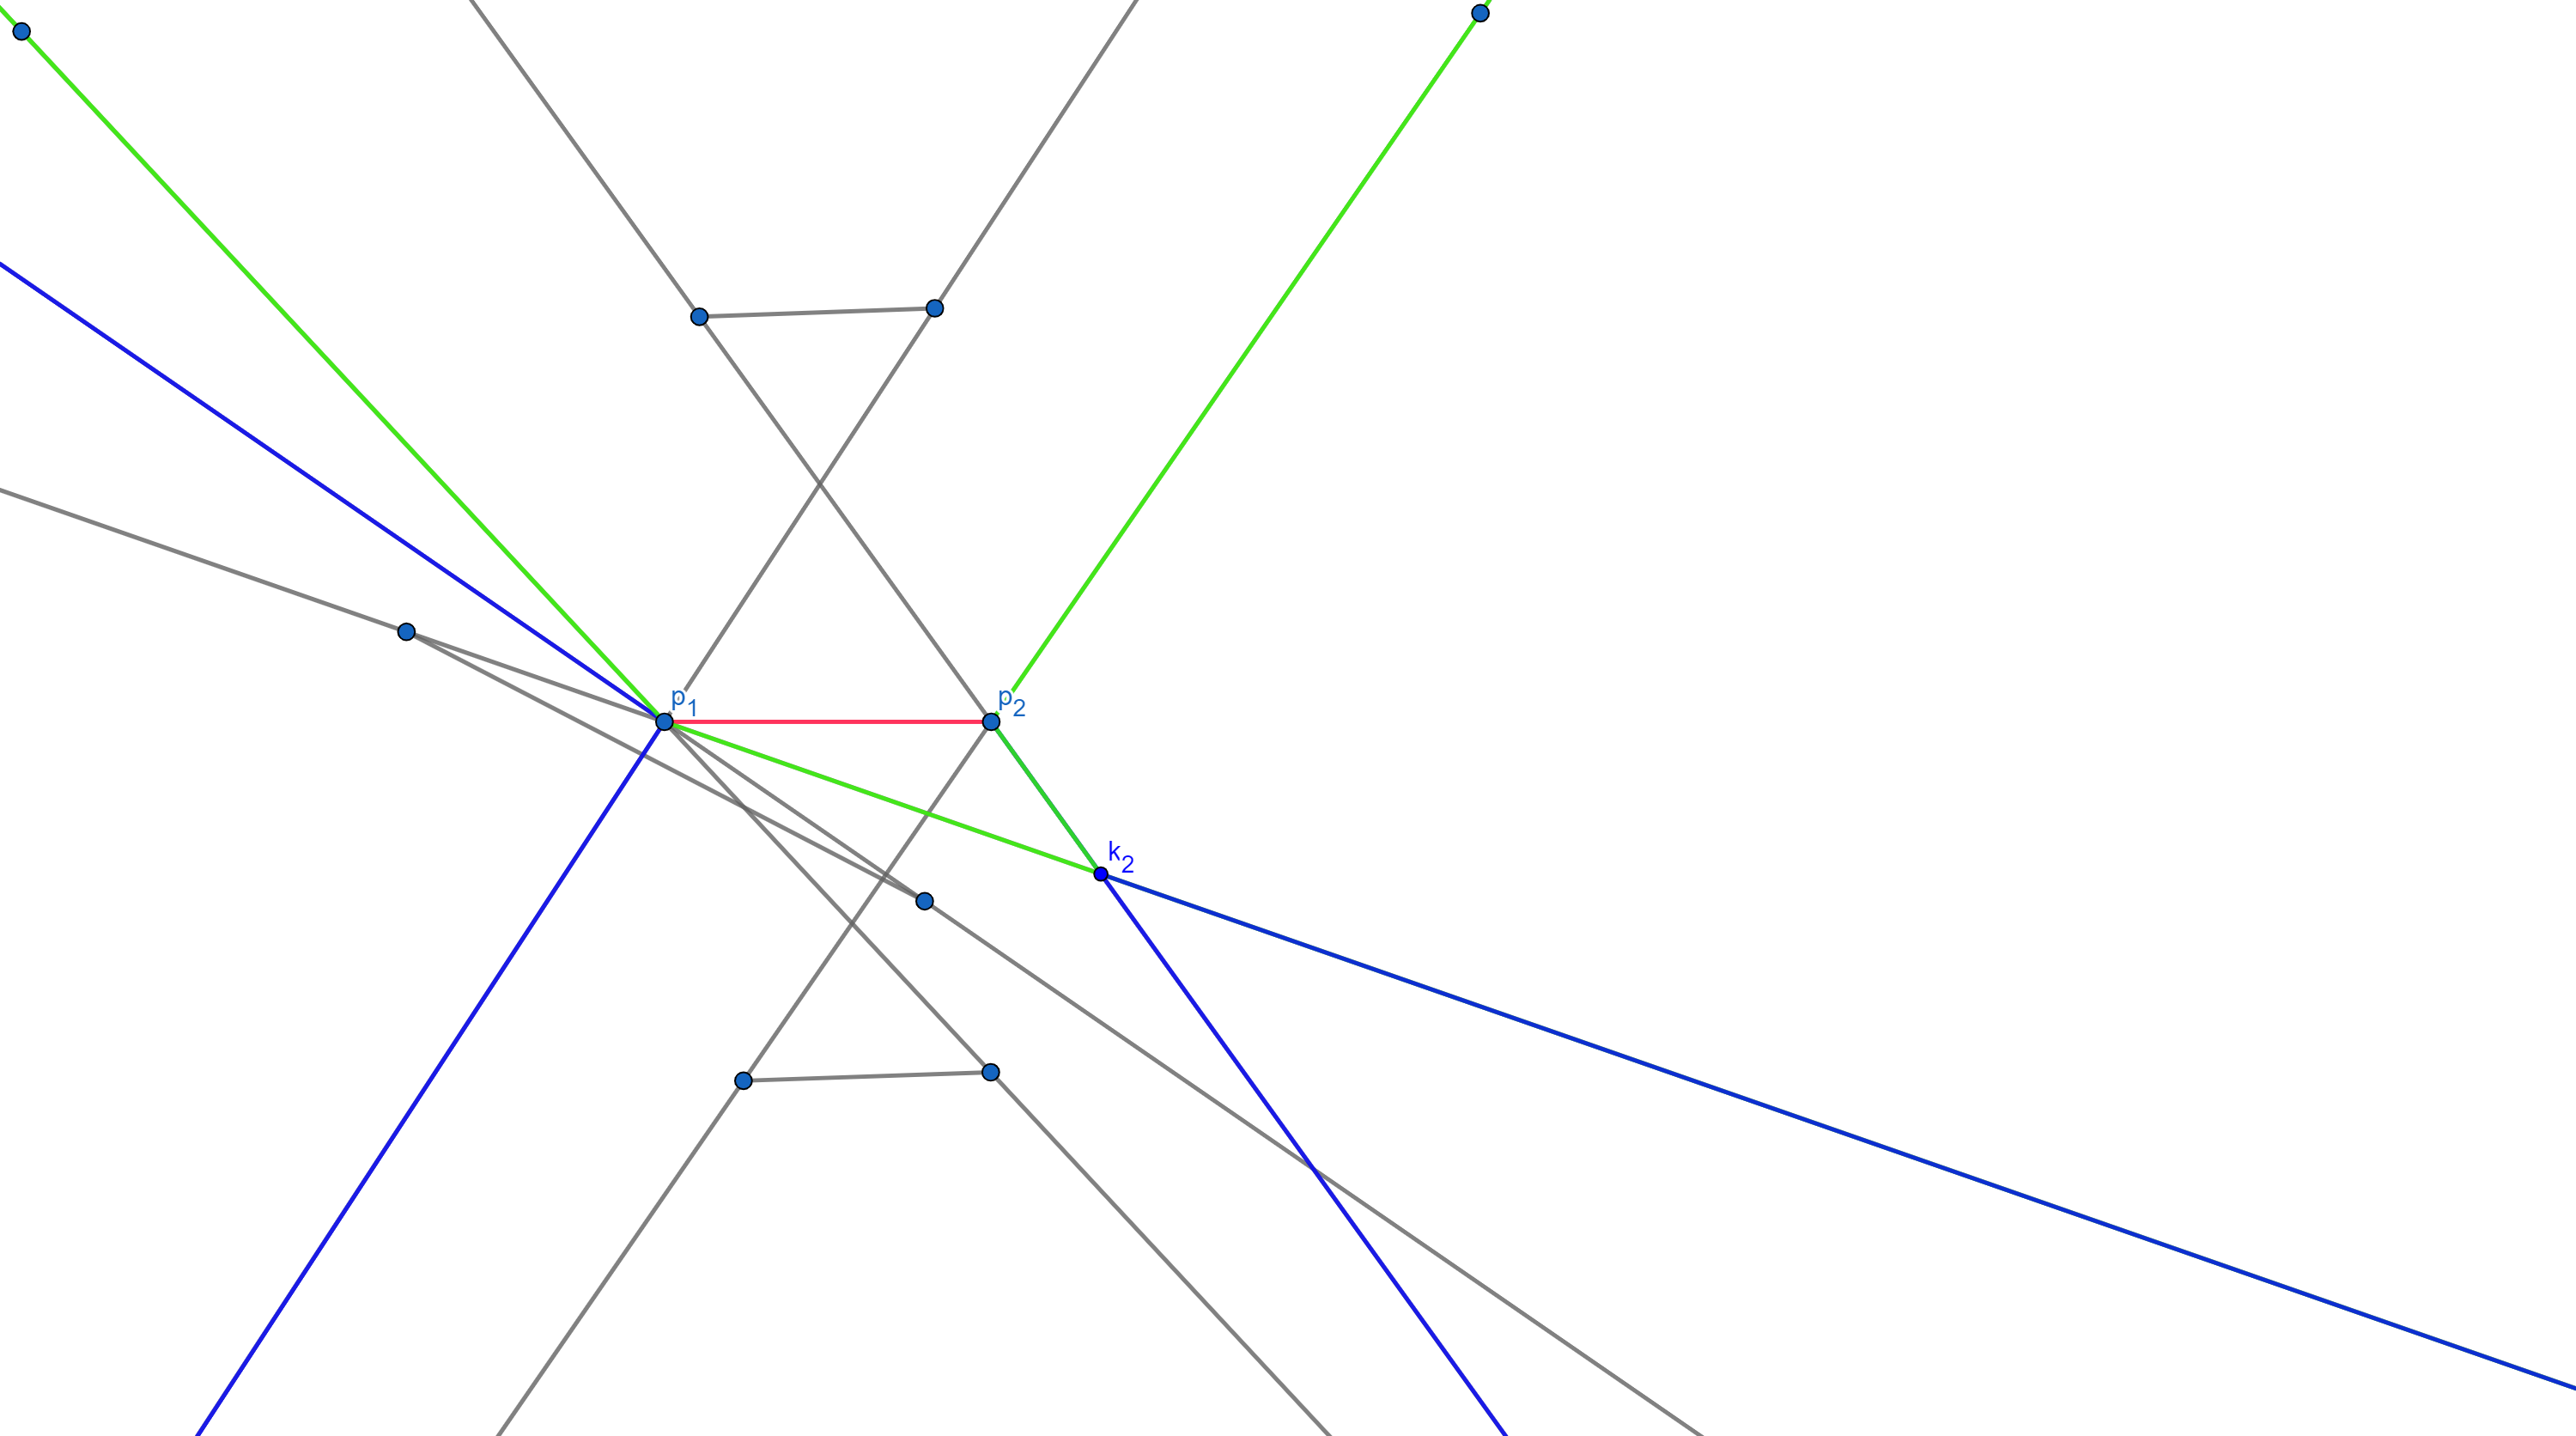
\includegraphics[width=0.5\linewidth]{nozone_3_4.png}
            \end{figure}
      \item Если все множества непустые, ограничения сводятся к 
            порождаемым аналогично предыдущему пункту точкам
            пересечения $k_1$, $k_2$, $k_3$, $k_4$.
            Итого результат: множество, ограниченное контрукциями
            луч-$k_1$-луч, луч-$k_2$-луч, луч-$k_3$-луч, луч-$k_4$-луч
            в любых комбинациях. От всей плоскости, до всех четырех.
            (16 вариантов, приведем несколько)
            \begin{figure}[H]
                  \centering
                  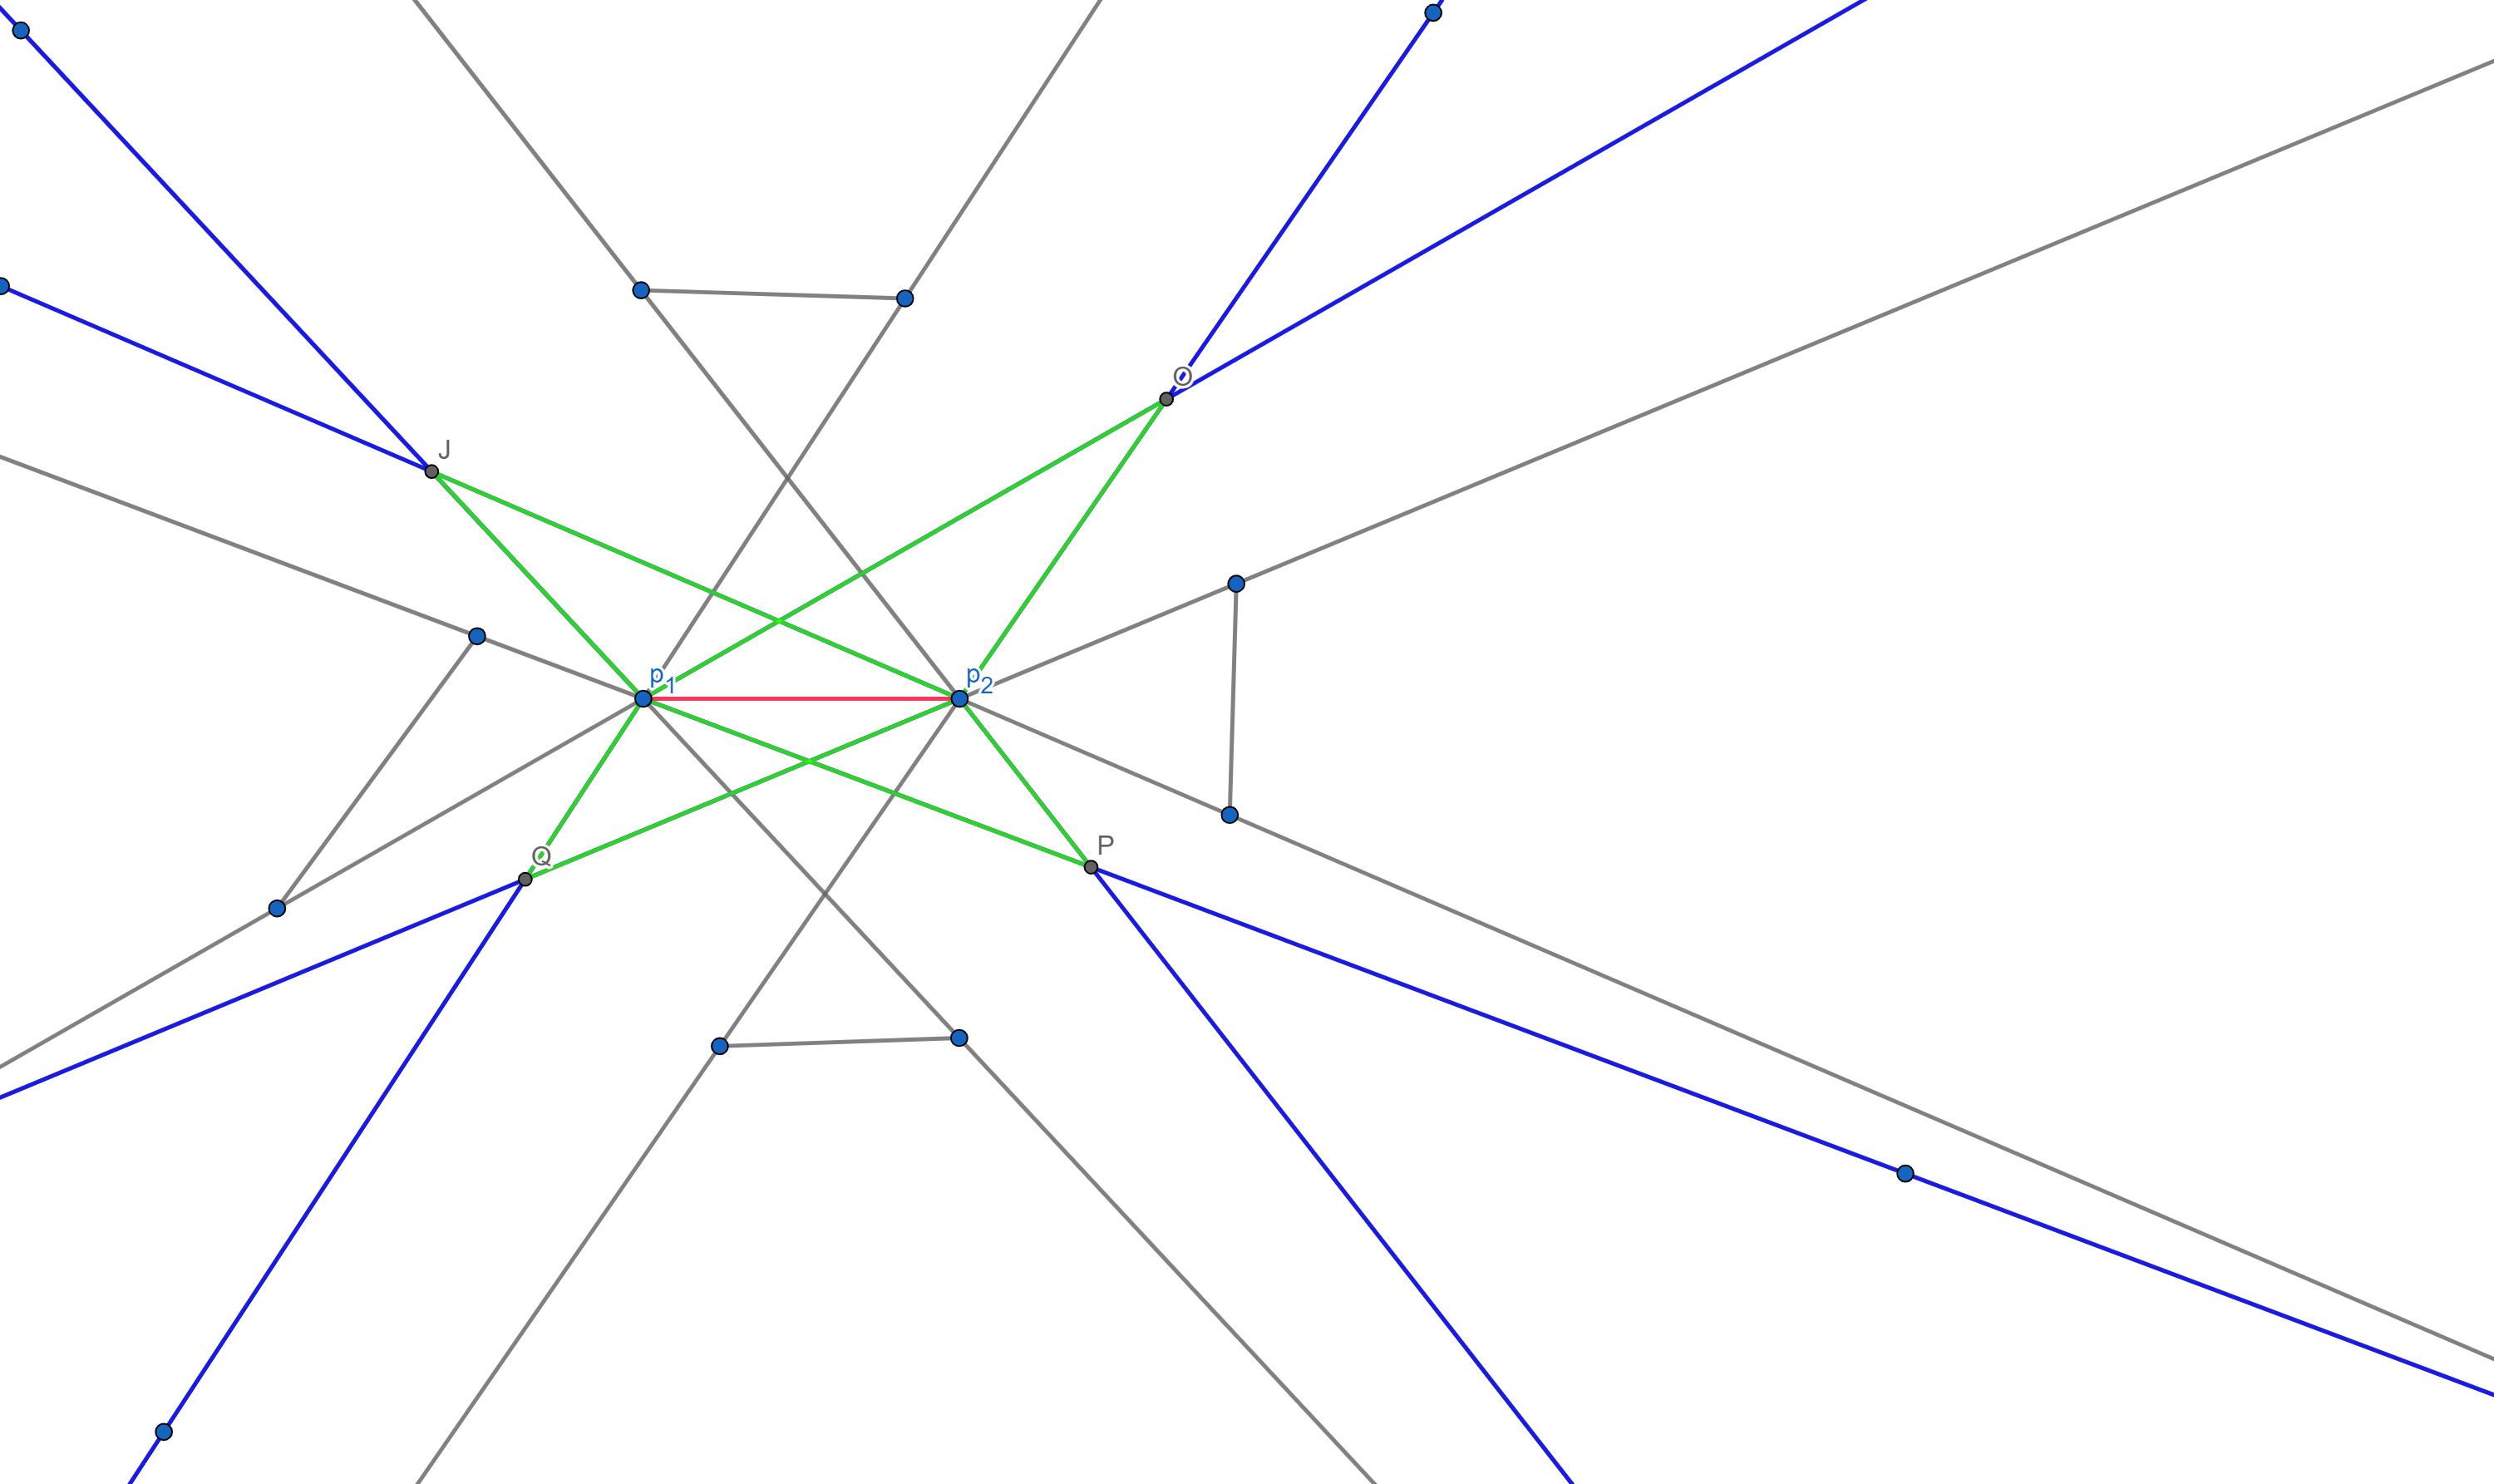
\includegraphics[width=0.5\linewidth]{nozone_4_1.png}
            \end{figure}
            \begin{figure}[H]
                  \centering
                  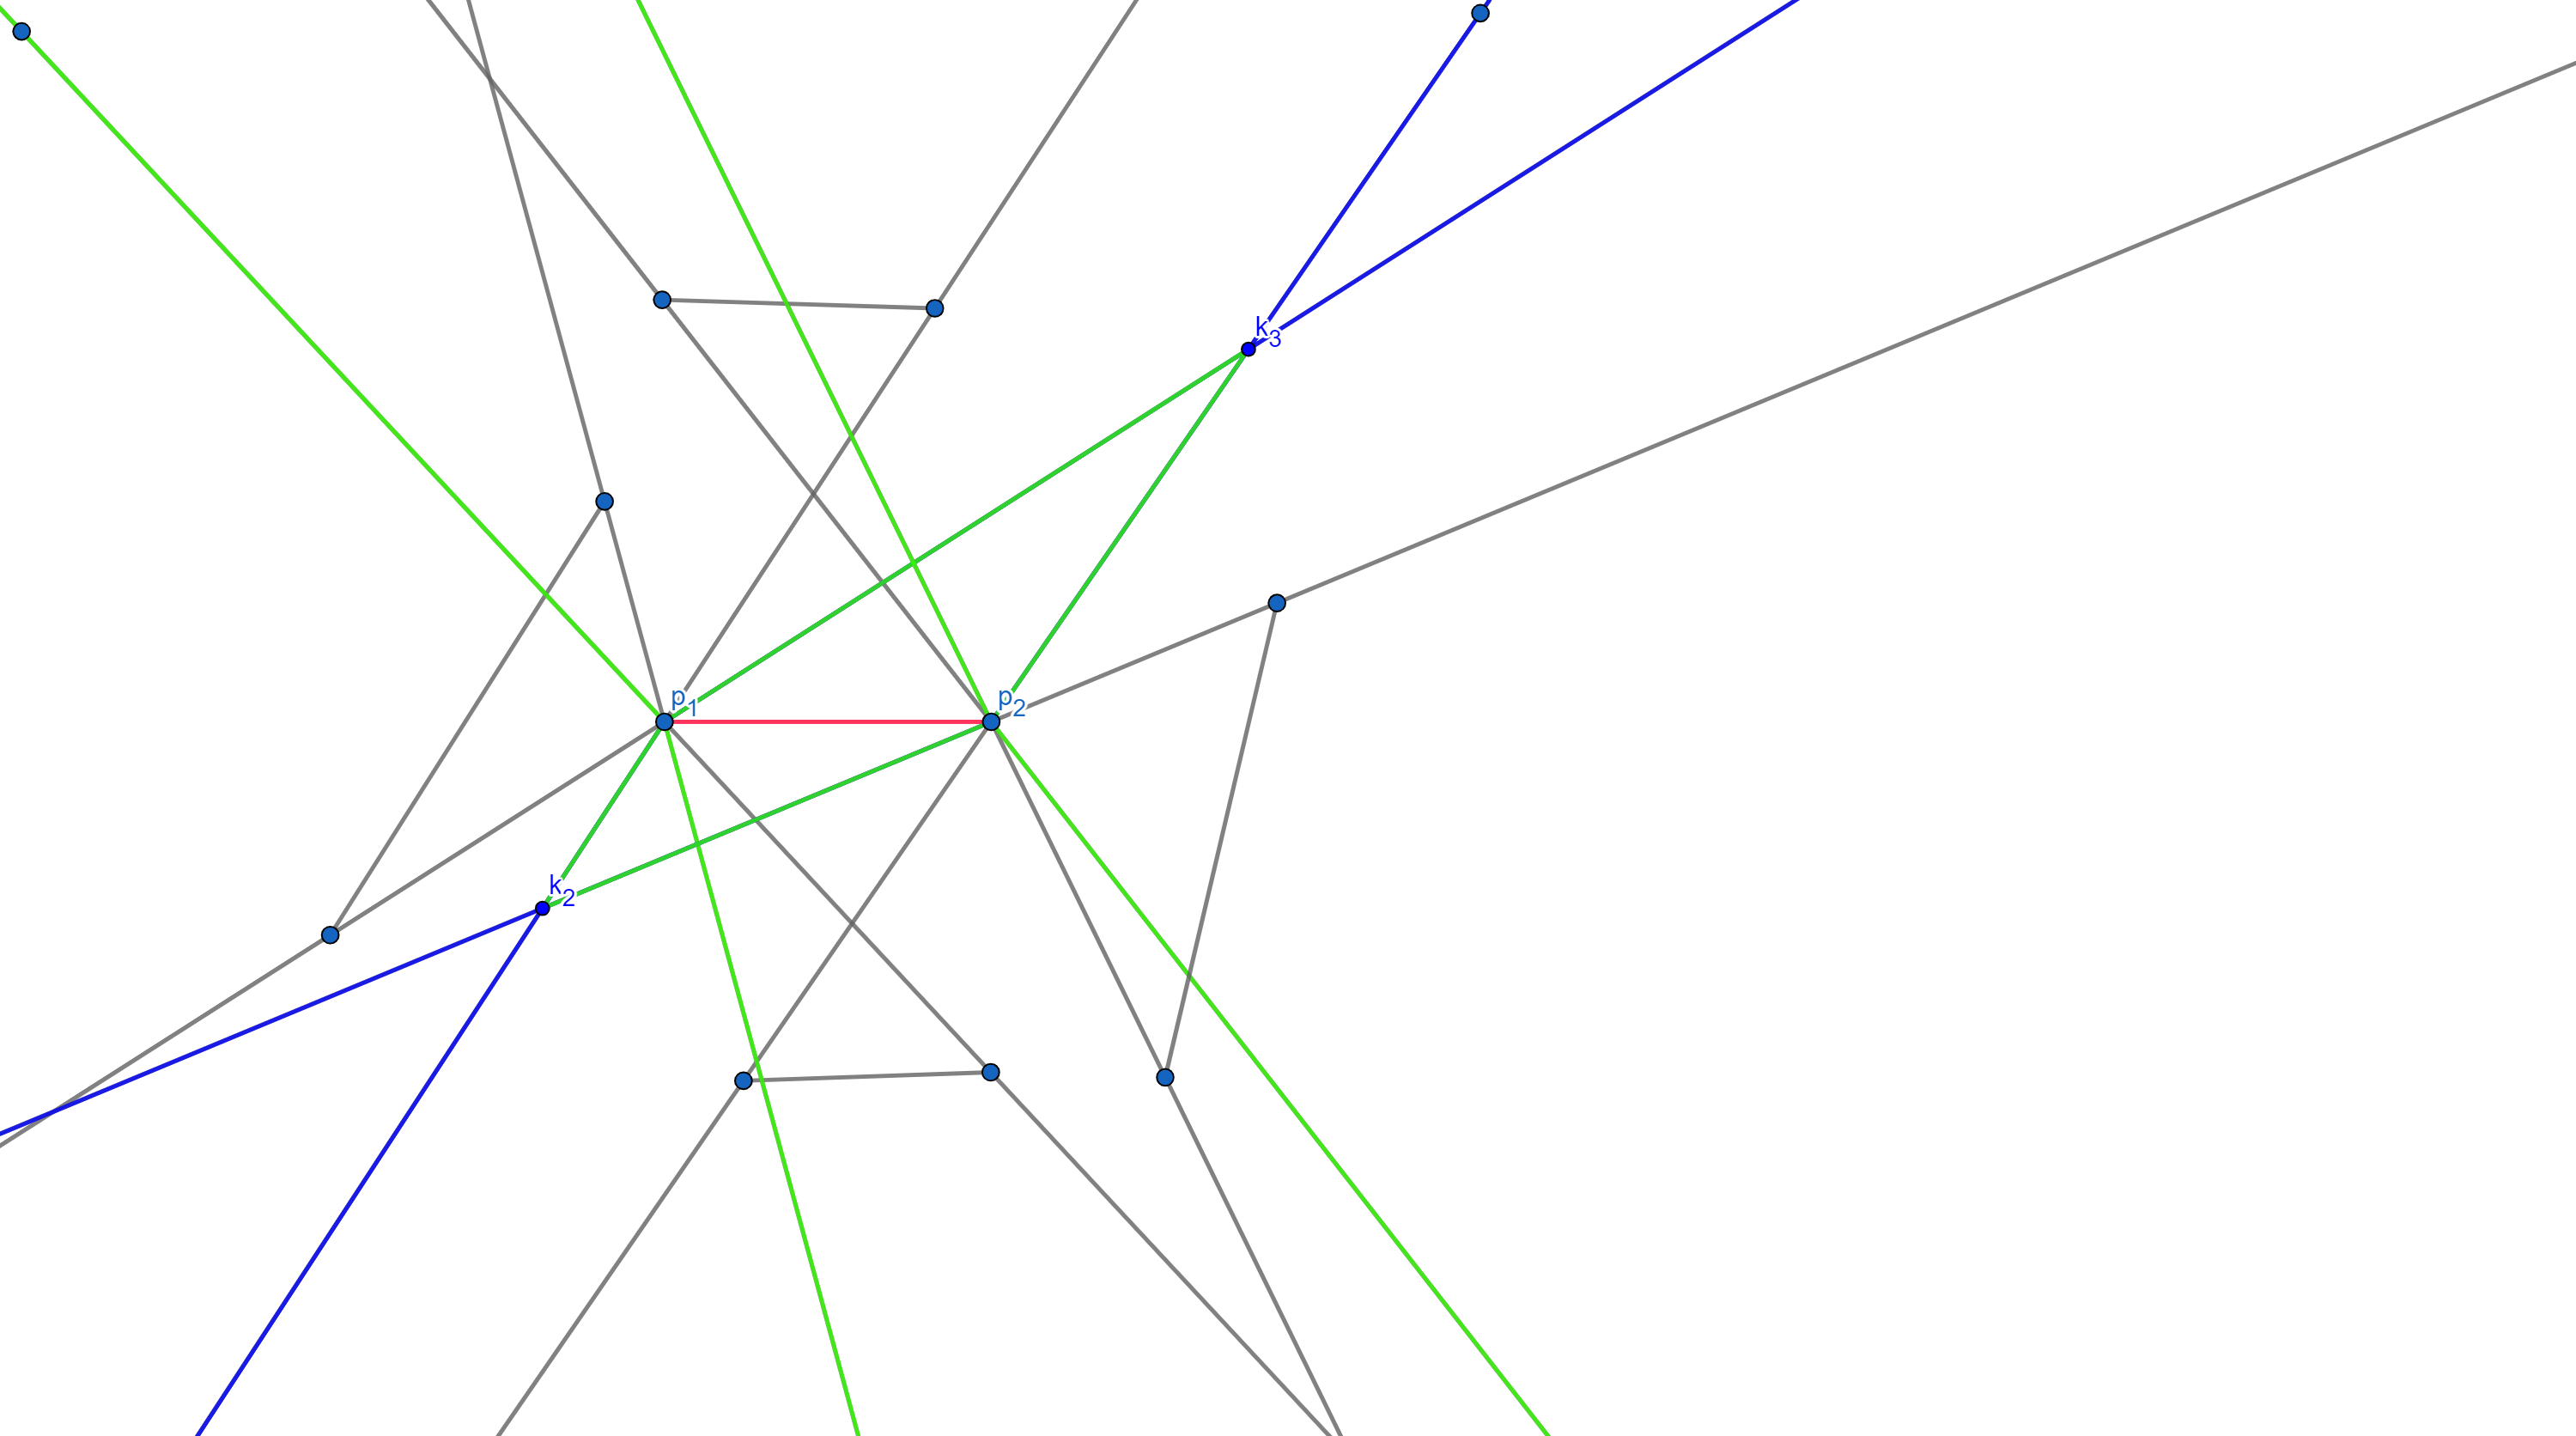
\includegraphics[width=0.5\linewidth]{nozone_4_2.png}
            \end{figure}
\end{enumerate}
Выводы:
\begin{enumerate}
      \item Построением всех <<нет-зоны>> заодно получены и 
            обратные им <<да-зоны>> (вернее не <<нет-зоны>>).
      \item Алгоритм построения таких зон можно реализовать за
            $O(n^2)$ в не зависимости от того, как именно искать
            пересечение плоскостей, так как их количество (0-10)
            ограничено. Основное время уйдет на поиск этих
            плоскостей.
      \item Выход такого алгоритма - <<да-зона>> отрезка,
            описанная как 0-4 конструкции луч-точка/отрезок-луч.
            Причем в случае отрезка лучи не пересекаются.
      \item Выход может быть пустым, если непусты 
            множества $S_3$, $S_4$ и одно из $S_1$, $S_2$.
\end{enumerate}
\end{document}